%!TEX root=./LIVRO.tex
\chapter[O alfabeto, as vogais e as consoantes]{\Large O alfabeto, as vogais e as consoantes}
\markboth{Módulo 1}{}

\section*{Habilidade do SAEB}

\begin{itemize}
\item Relacionar elementos sonoros das palavras com sua representação escrita.
\end{itemize}

\subsection{Habilidade da BNCC}

\begin{itemize}
\item EF02LP03.
\end{itemize}

\conteudo{Para escrever as palavras, usamos as \textbf{letras}. 
Ao todo, temos 26 letras na língua portuguesa. Juntas, elas compõem o \textbf{alfabeto}.

As \textbf{vogais} são \textit{a, e, i, o, u}. As outras letras, denominadas
\textbf{consoantes}, são:

\begin{center}
\textsc{b c d f g h j k l m n p q r s t v w x y z}\hfill
\end{center}

Cada letra possui um nome e um som, que, quando estão juntos, podem
formar muitas palavras.

Algumas letras podem também apresentar sons diferentes a partir do contexto em que são utilizadas. A letra C, por exemplo, possui dois sons diferentes de acordo com a vogal que
acompanha. Por exemplo: junto com as vogais A, O e U, apresenta o som de 
/k/; junto com E e I, apresenta o som de /s/.
 
%Felipe: precisamos padronizar como vamos grafar as letras e os fonemas, como ocorreu na frase acima. (Rogério, 13/3/23, 14h31)

\textbf{Palavras com som de /k/:} cuca, casa e coco.

\textbf{Palavras com som de /s/:} cebola, cinco e cisne.

Algumas palavras com o som de /k/ também podem ser escritas com Q,
mas vale lembrar que o Q vem sempre acompanhado de U e de mais uma
vogal, e é esta última vogal que vai marcar o som da sílaba.

\textbf{Palavras com /qu:} queijo, quilo e quero.

Veja a grafia dessas palavras.

TAT\textbf{U} GAL\textbf{O} 

Na grafia das palavras com as vogais O e U, o O final é pronunciado de maneira
fraca, enquanto o U é sempre forte.
}

%\pagebreak

\section*{Atividades}

\num{1} Complete os nomes das figuras com as letras que estão faltando.

\begin{table}[H]
\centering
\begin{tabular}{ll}
\multicolumn{1}{c}{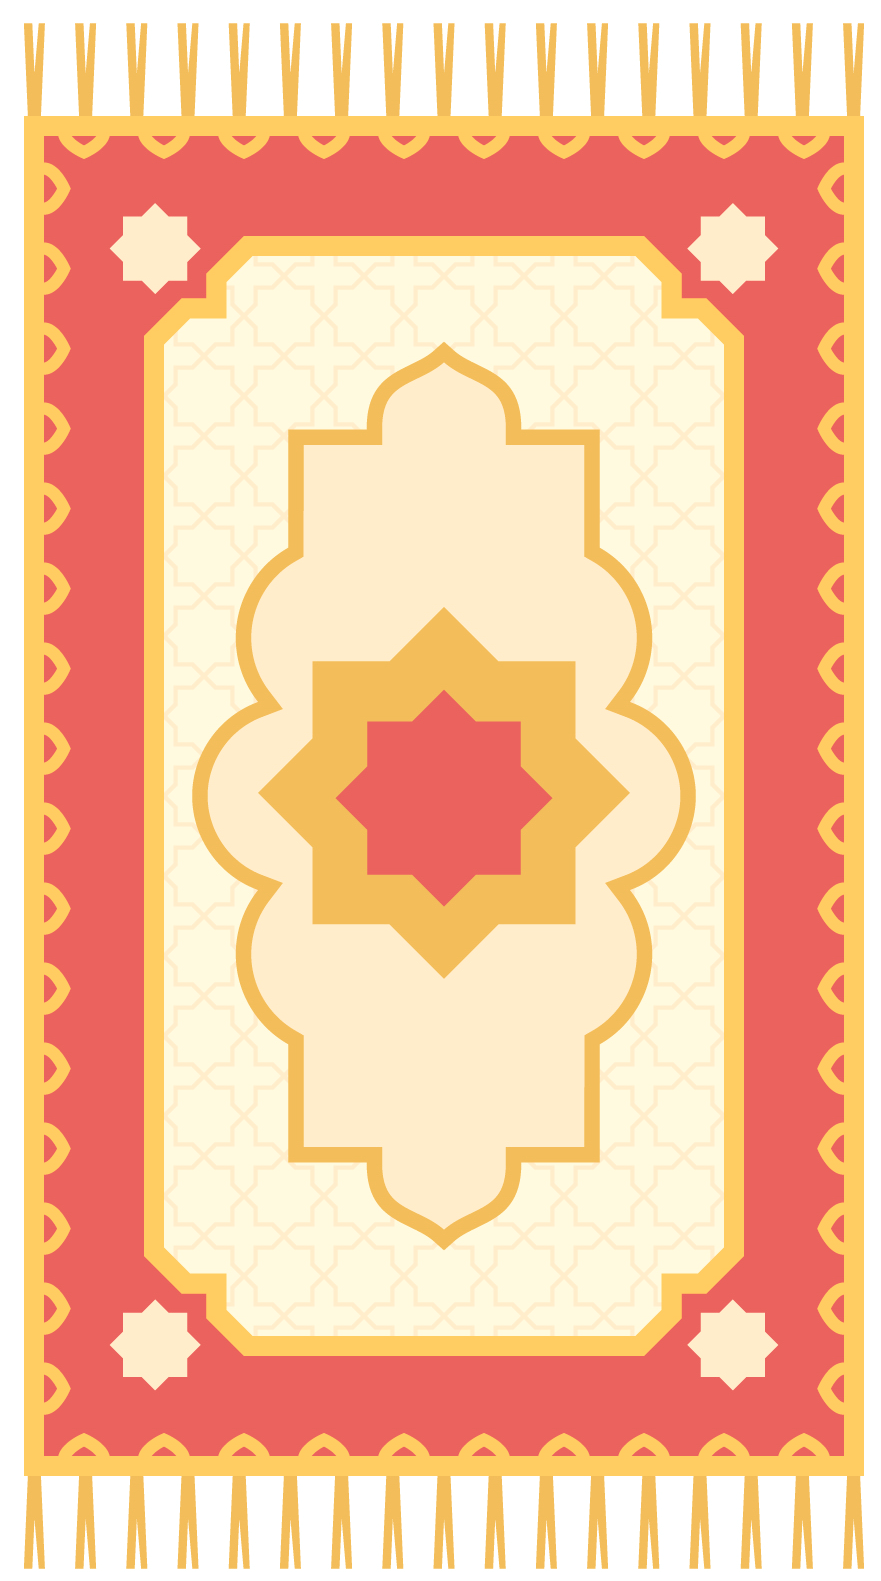
\includegraphics[width=.25\textwidth]{media/image1.png}} & \multicolumn{1}{c}{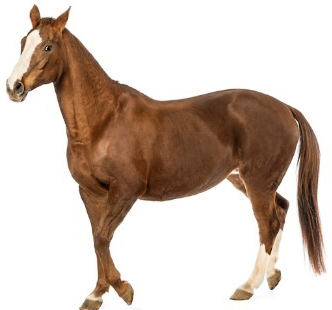
\includegraphics[width=.35\textwidth]{media/image2.png}} \\
\multicolumn{1}{c}{\textbf{T \reduline{A} P \reduline{E} T \reduline{E}}} & \multicolumn{1}{c}{\textbf{C \reduline{A} V \reduline{A} L \reduline{O}}}
\end{tabular}
\end{table}

\begin{table}[H]
\centering
\begin{tabular}{ll}
\multicolumn{1}{c}{
\includegraphics[width=.4\textwidth]{media/image3.jpeg}} & \multicolumn{1}{c}{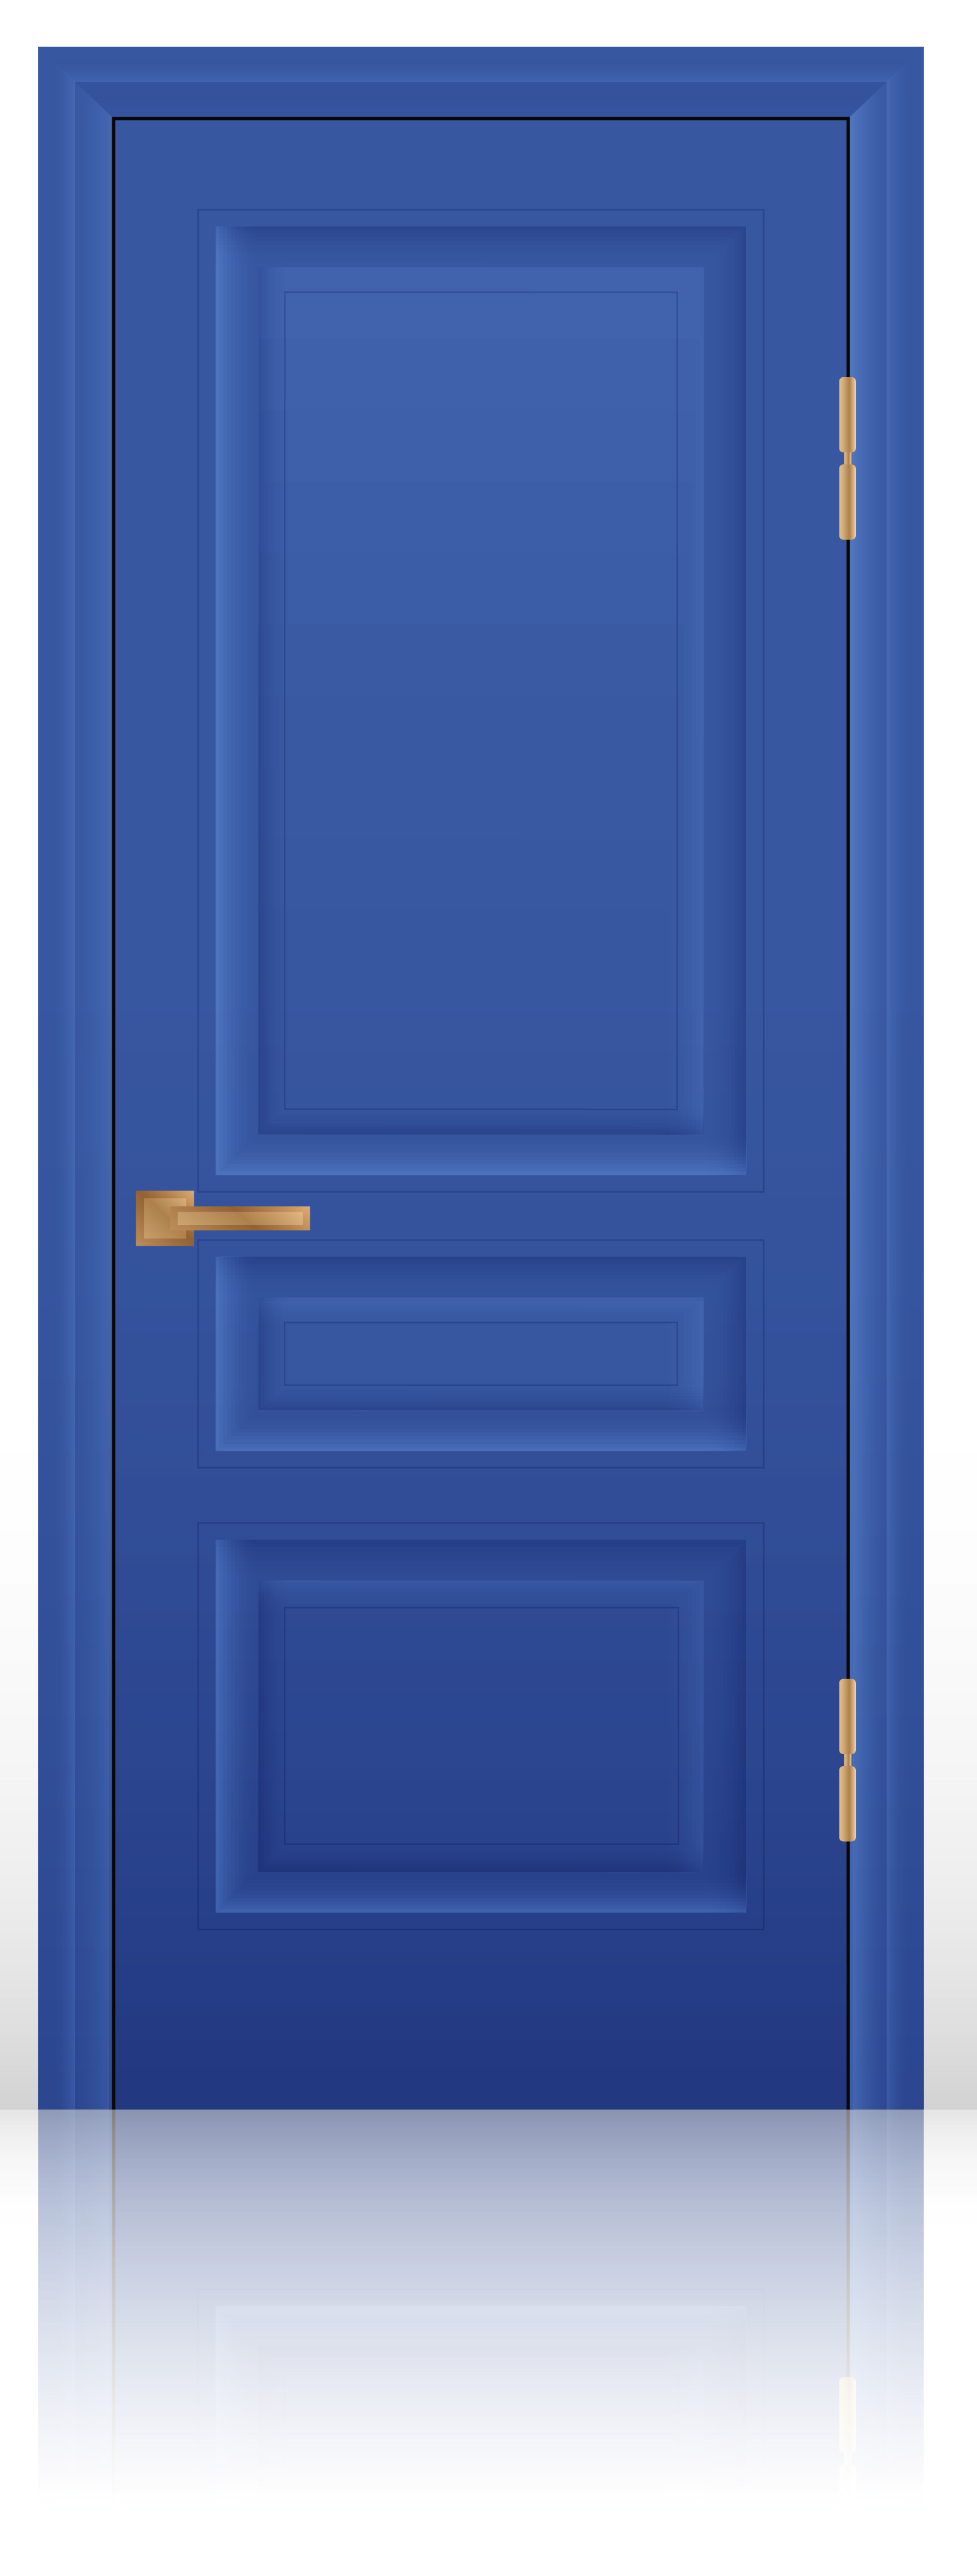
\includegraphics[width=.2\textwidth]{media/image4.png}} \\
\multicolumn{1}{c}{\textbf{\reduline{E} STR \reduline{E} L \reduline{A}}} & \multicolumn{1}{c}{\textbf{P \reduline{O} RT \reduline{A}}}
\end{tabular}
\end{table}

Você completou as palavras com

\begin{boxlist}
\boxitem{\white{X}} Vogais 

\boxitem{\white{X}} Consoantes
\end{boxlist}

%\coment{Apresente as vogais em cartaz. Pergunte o nome dos objetos representados nas imagens e, em seguida, convide as crianças para montar as palavras no alfabeto móvel para identificar as letras faltantes.}

\num{2} Complete o alfabeto com as letras que estão faltado.

\begin{center}
\Large
\begin{tabular}{|l|l|llllll}
\hline
\textbf{A} & \rosa{B} & \multicolumn{1}{l|}{\rosa{C}} & \multicolumn{1}{l|}{\rosa{D}} & \multicolumn{1}{l|}{\textbf{E}} & \multicolumn{1}{l|}{\rosa{F}} & \multicolumn{1}{l|}{\rosa{G}} & \multicolumn{1}{l|}{\rosa{H}} \\ \hline
\textbf{I} & \rosa{J} & \multicolumn{1}{l|}{\rosa{K}} & \multicolumn{1}{l|}{\rosa{L}} & \multicolumn{1}{l|}{\rosa{M}} & \multicolumn{1}{l|}{\rosa{N}} & \multicolumn{1}{l|}{\textbf{O}} & \multicolumn{1}{l|}{\rosa{P}} \\ \hline
\rosa{Q} & \rosa{R} & \multicolumn{1}{l|}{\rosa{S}} & \multicolumn{1}{l|}{\rosa{T}} & \multicolumn{1}{l|}{\textbf{U}} & \multicolumn{1}{l|}{\rosa{V}} & \multicolumn{1}{l|}{\rosa{W}} & \multicolumn{1}{l|}{\rosa{X}} \\ \hline
\rosa{Y} & \rosa{Z} & \textbf{} & \textbf{} & \textbf{} & \textbf{} & \textbf{} & \textbf{} \\ \cline{1-2}
\end{tabular}
\end{center}

Você completou os quadradinhos com:

\begin{boxlist}
\boxitem{\white{X}} Vogais 

\boxitem{\white{X}} Consoantes
\end{boxlist}

%\coment{Leve o alfabeto móvel para sala e convide os alunos para organizar as letras na ordem certa. Em seguida, oriente-os a preencher o quadro; depois ajude a separar vogais e consoantes.}

\num{3} Leia o poema.

\begin{myquote}
\begin{center}
\textbf{A vaca Filomena e a formiga Violeta}\\
\end{center}

\begin{verse}
A vaca Filomena\\
mora na vila formosa.\\
A formiga Violeta\\
mora na cerca cor de rosa.

A vaca Filomena\\
come as uvas da parreira.\\
A formiga Violeta\\
acha isto uma besteira.
\end{verse}

\fonte{Isabel Cristina Silveira Soares. https://seceducacao.padua.rj.gov.br/wp-content/uploads/2021/05/3o-ano-Ling.-Portuguesa-ATIV.17.pdf.
Acesso 28 de Fev 2023.}
\end{myquote}

Encontre e pinte no texto todas as palavras iniciadas com F e V. 
Depois escreva abaixo as palavras que encontrou.

\reduline{As palavras encontradas são as seguintes: vaca, Filomena, vila,
formosa, formiga, violeta.\hfill}

\pagebreak

\num{4} Complete os espaços a seguir com as letras iniciais das palavras
\textit{violeta} e \textit{Filomena}.

%\coment{Leve as palavras Violeta e Filomena em um cartaz. Explore a letra inicial e o som da letra nas palavras.}

\begin{table}[H]
\begin{tabular}{ll}
\multicolumn{1}{c}{
\includegraphics[width=.55\textwidth]{media/image14.jpg}} & \multicolumn{1}{c}{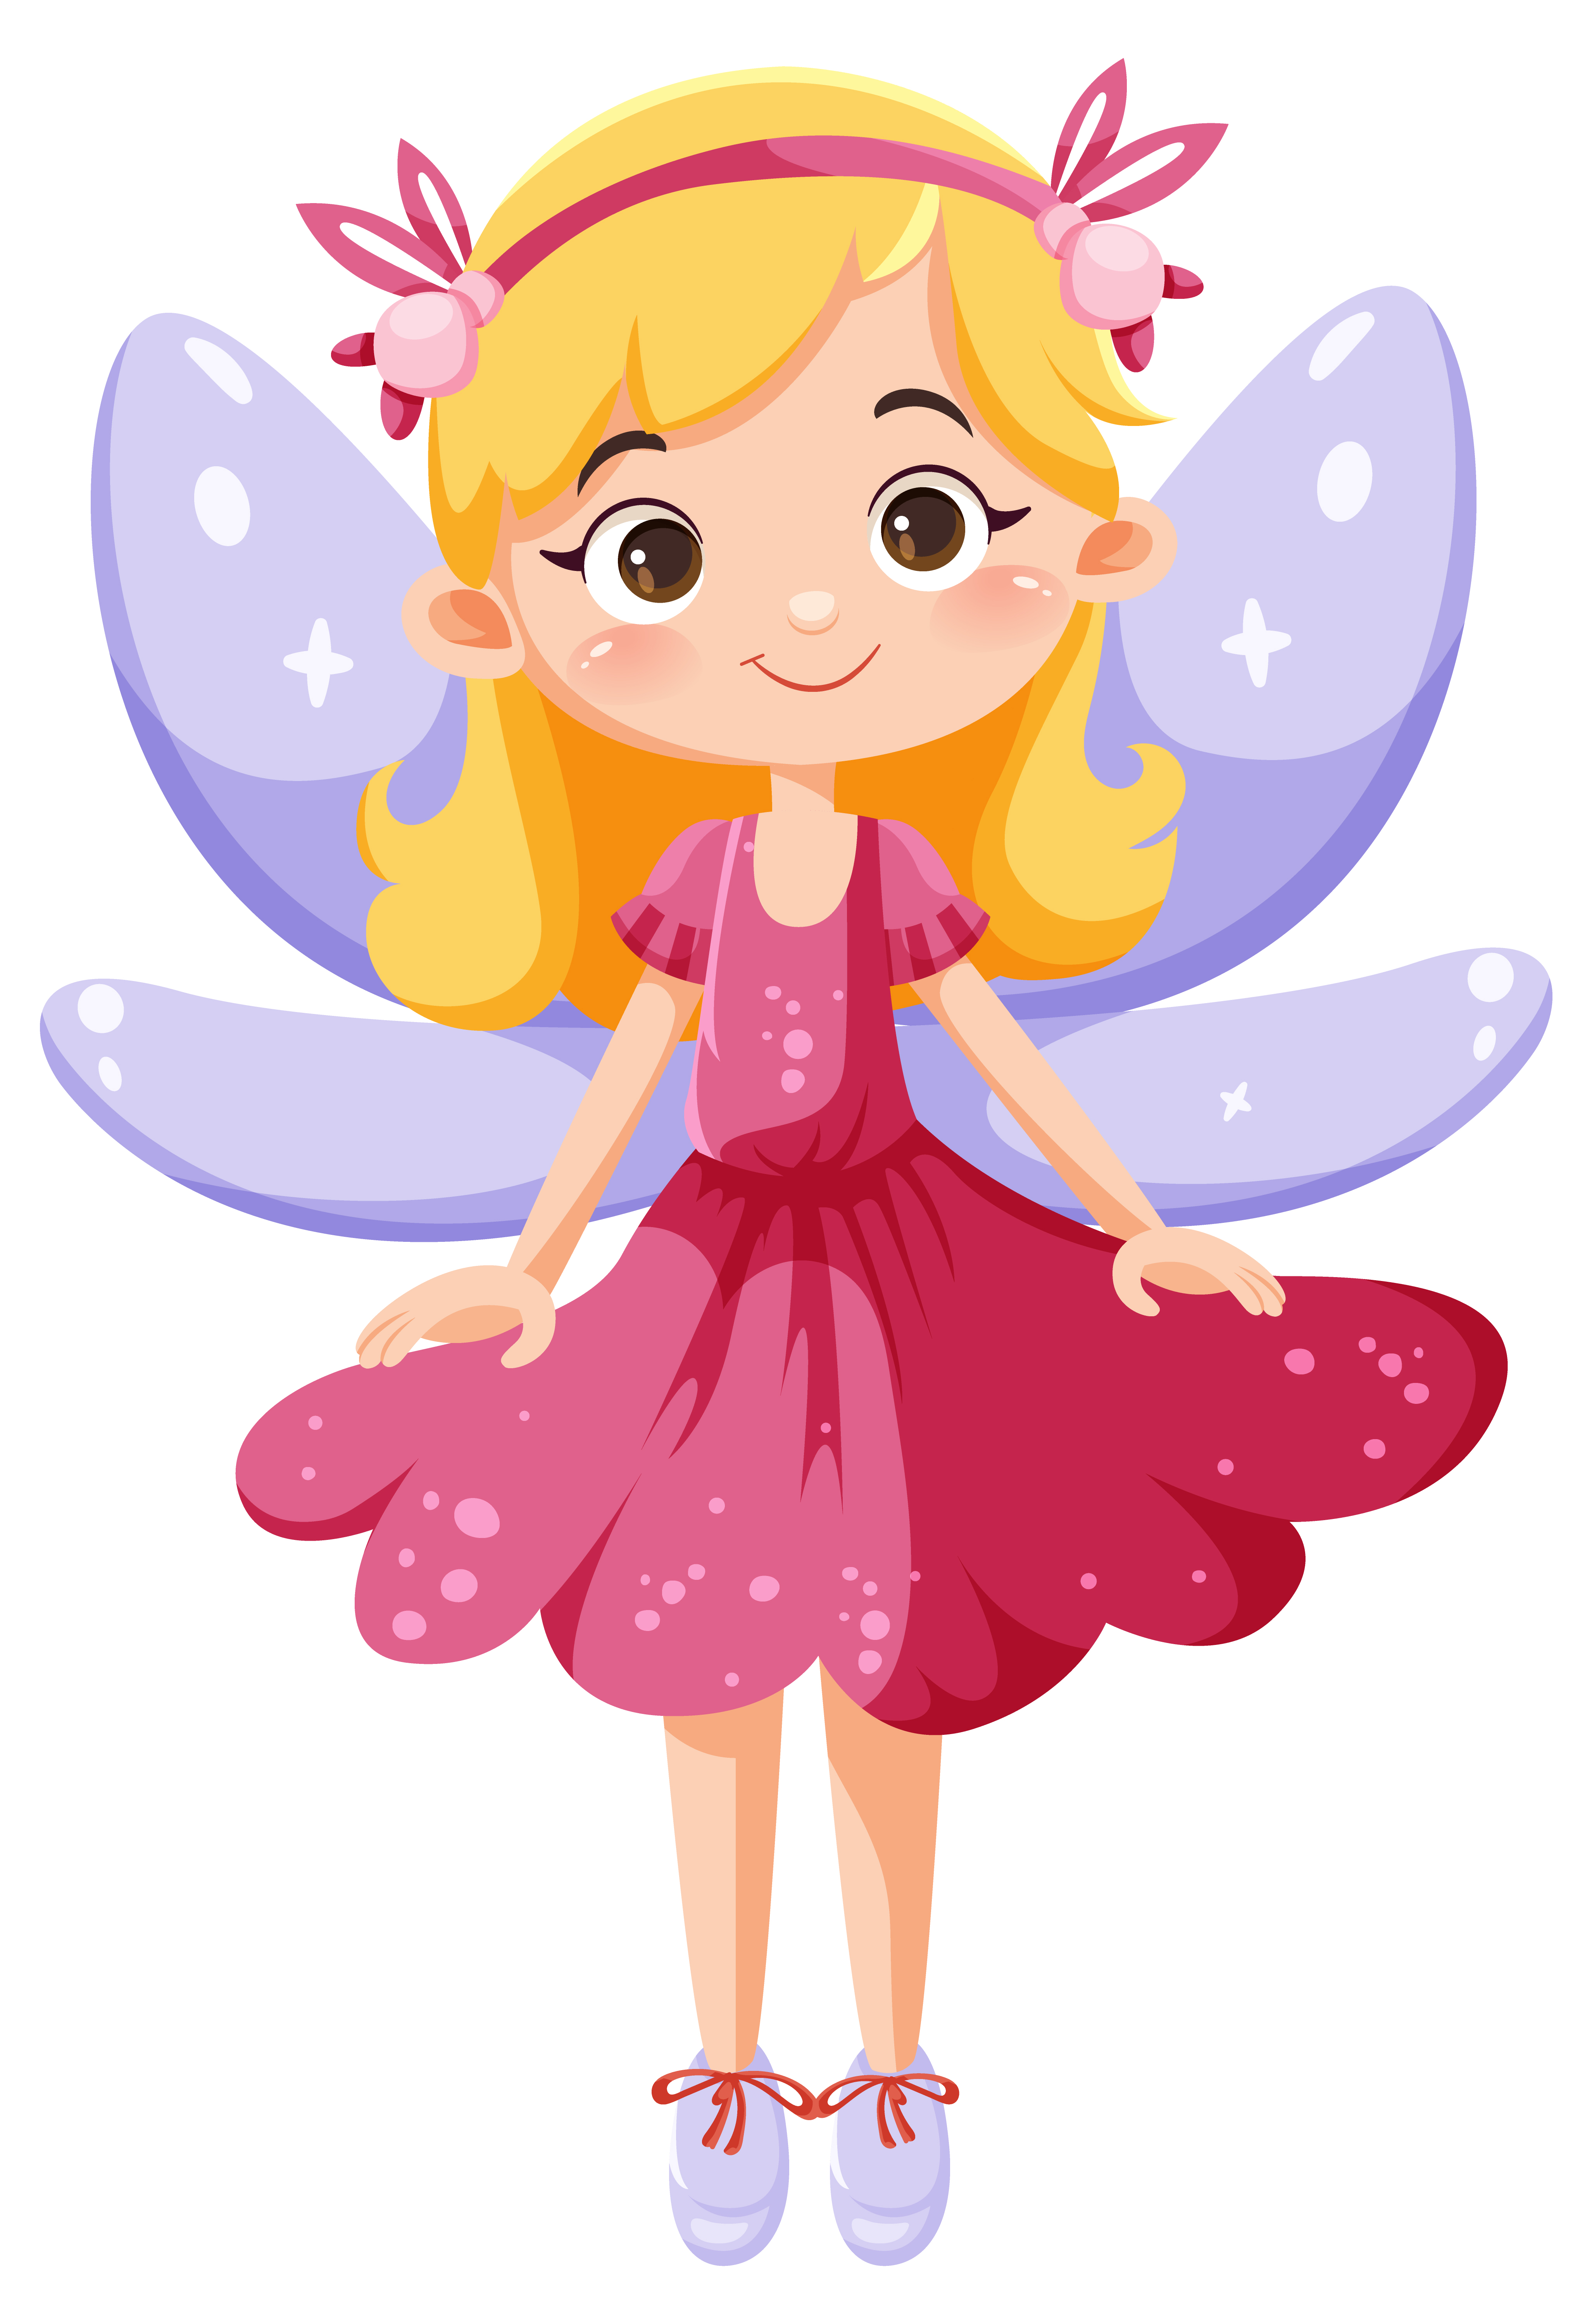
\includegraphics[width=.35\textwidth]{media/image8.jpg}} \\
\multicolumn{1}{c}{\textbf{\reduline{F} OGUETE}} & \multicolumn{1}{c}{\textbf{\reduline{F} ADA}}
\end{tabular}
\end{table}

\vspace*{+1em}

\begin{table}[H]
\begin{tabular}{ll}
\multicolumn{1}{c}{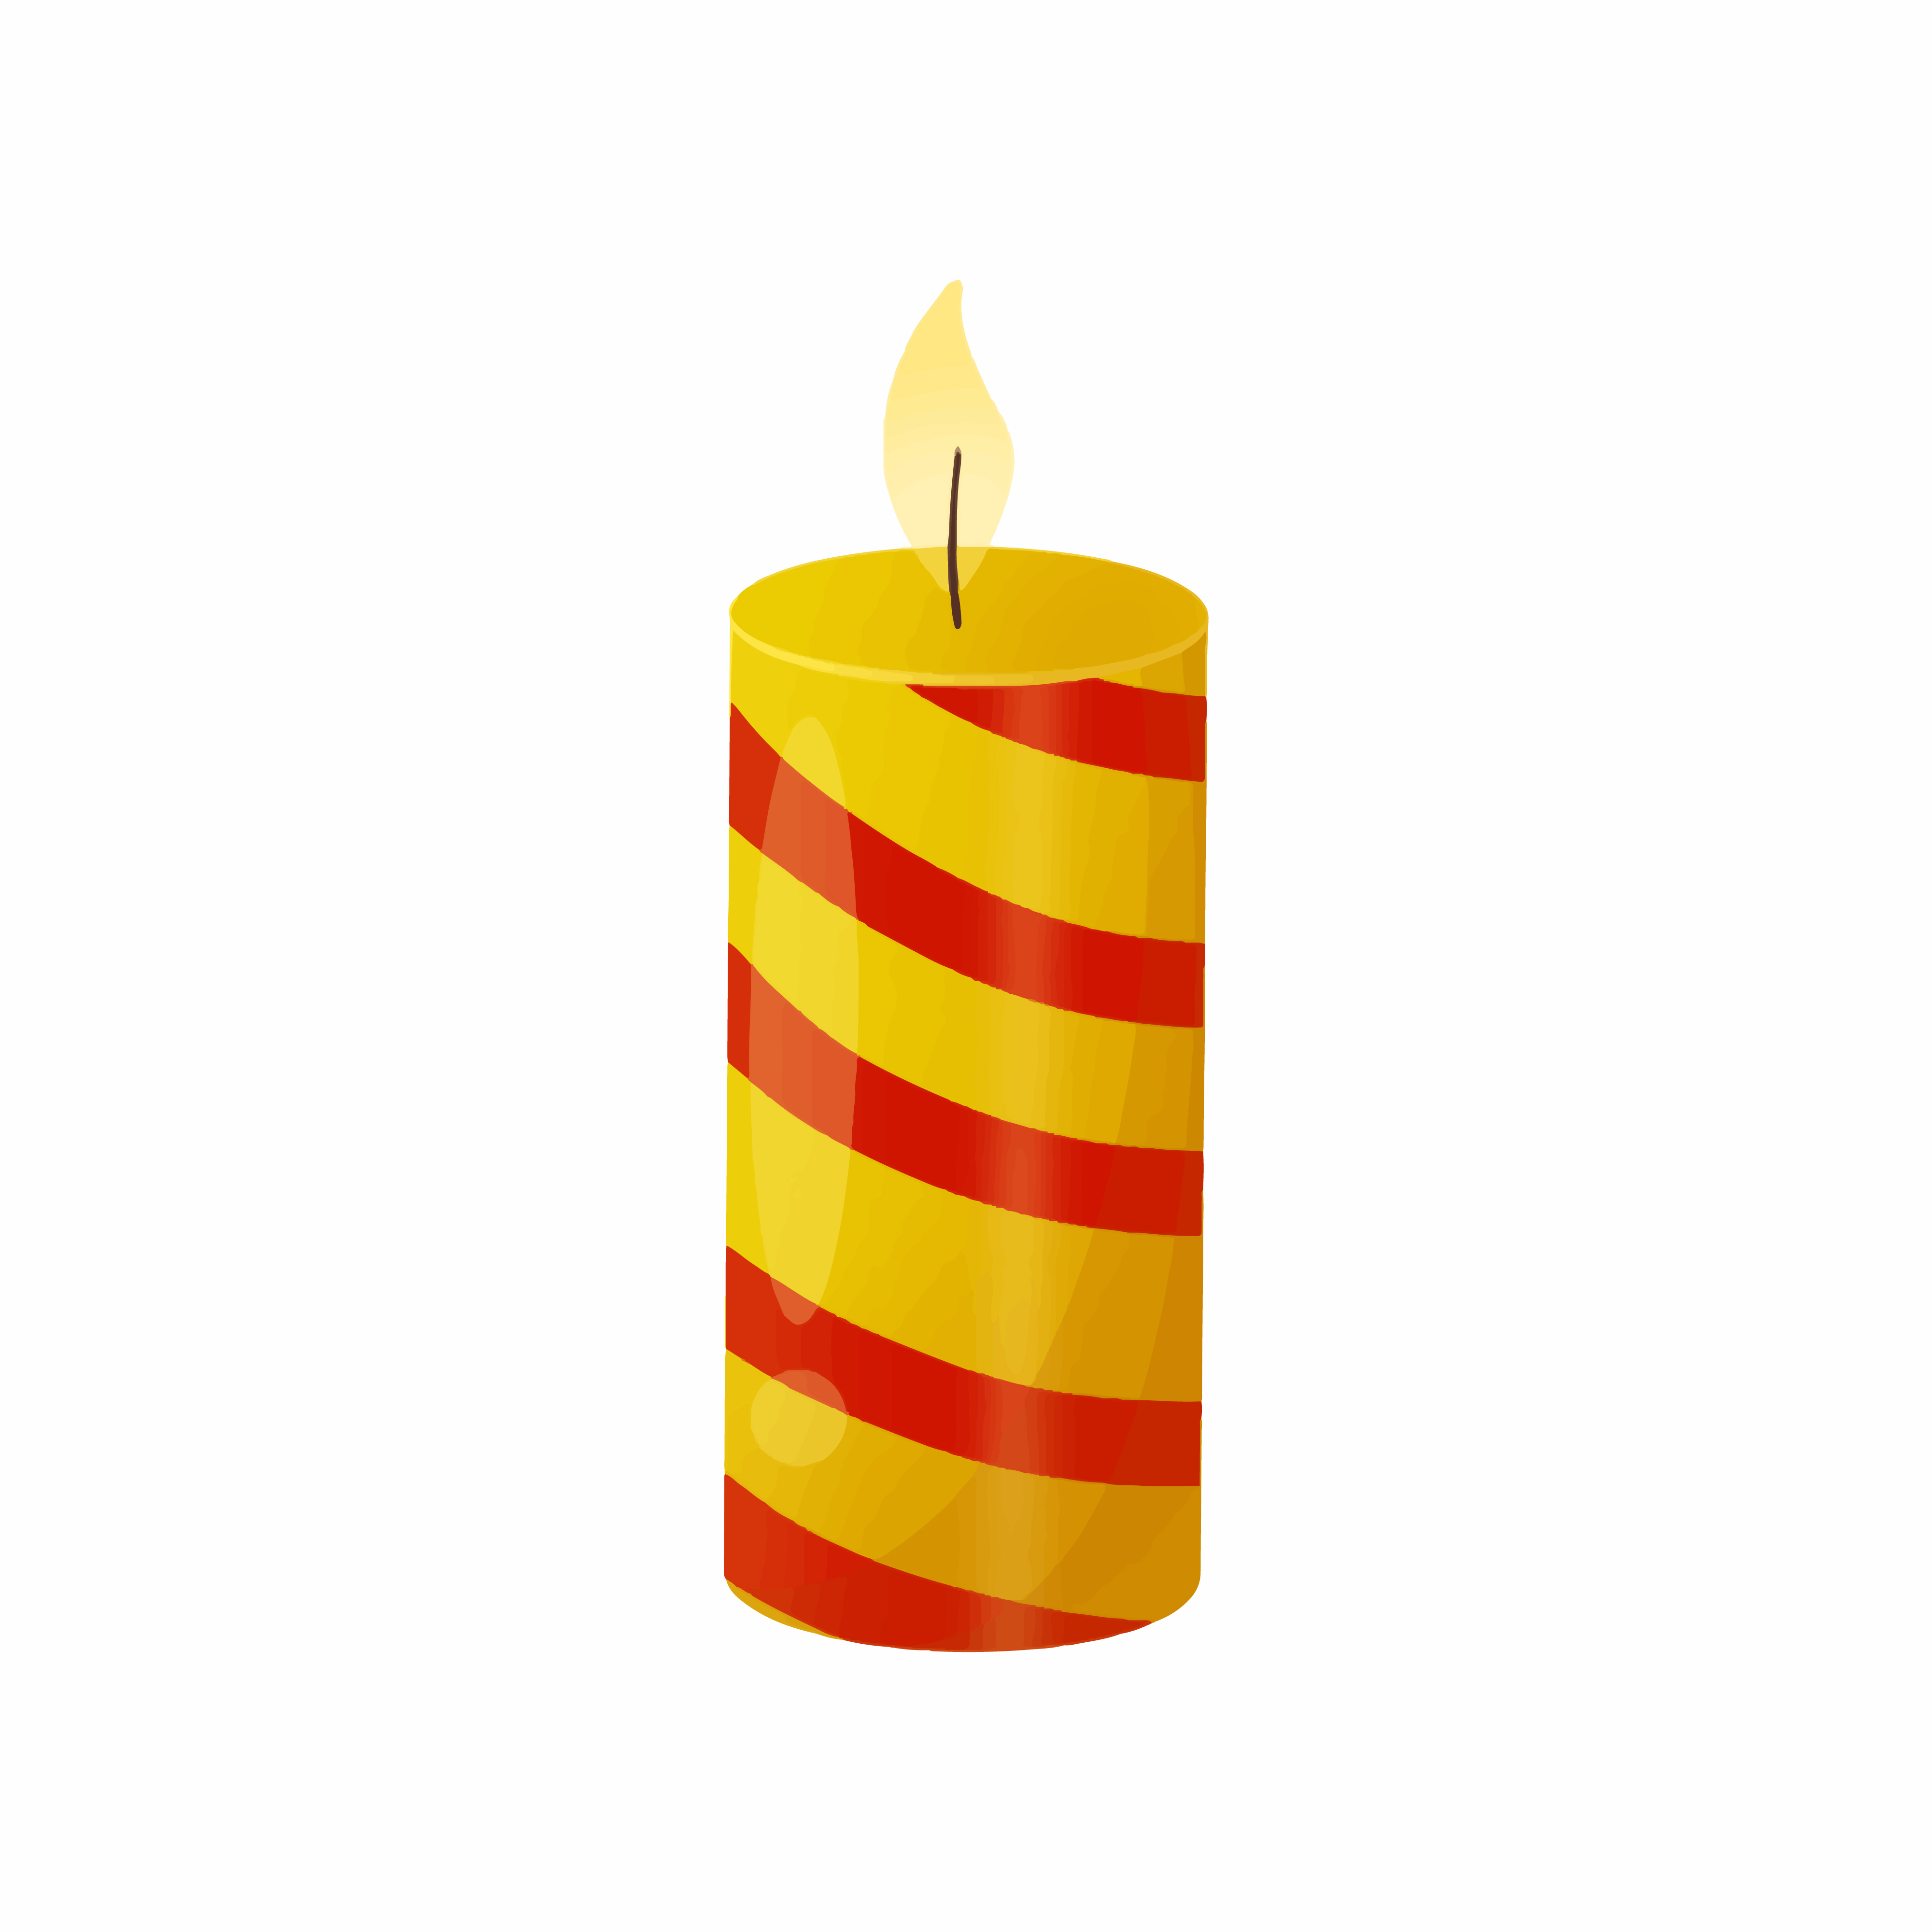
\includegraphics[width=.55\textwidth]{media/image9.jpg}} & \multicolumn{1}{c}{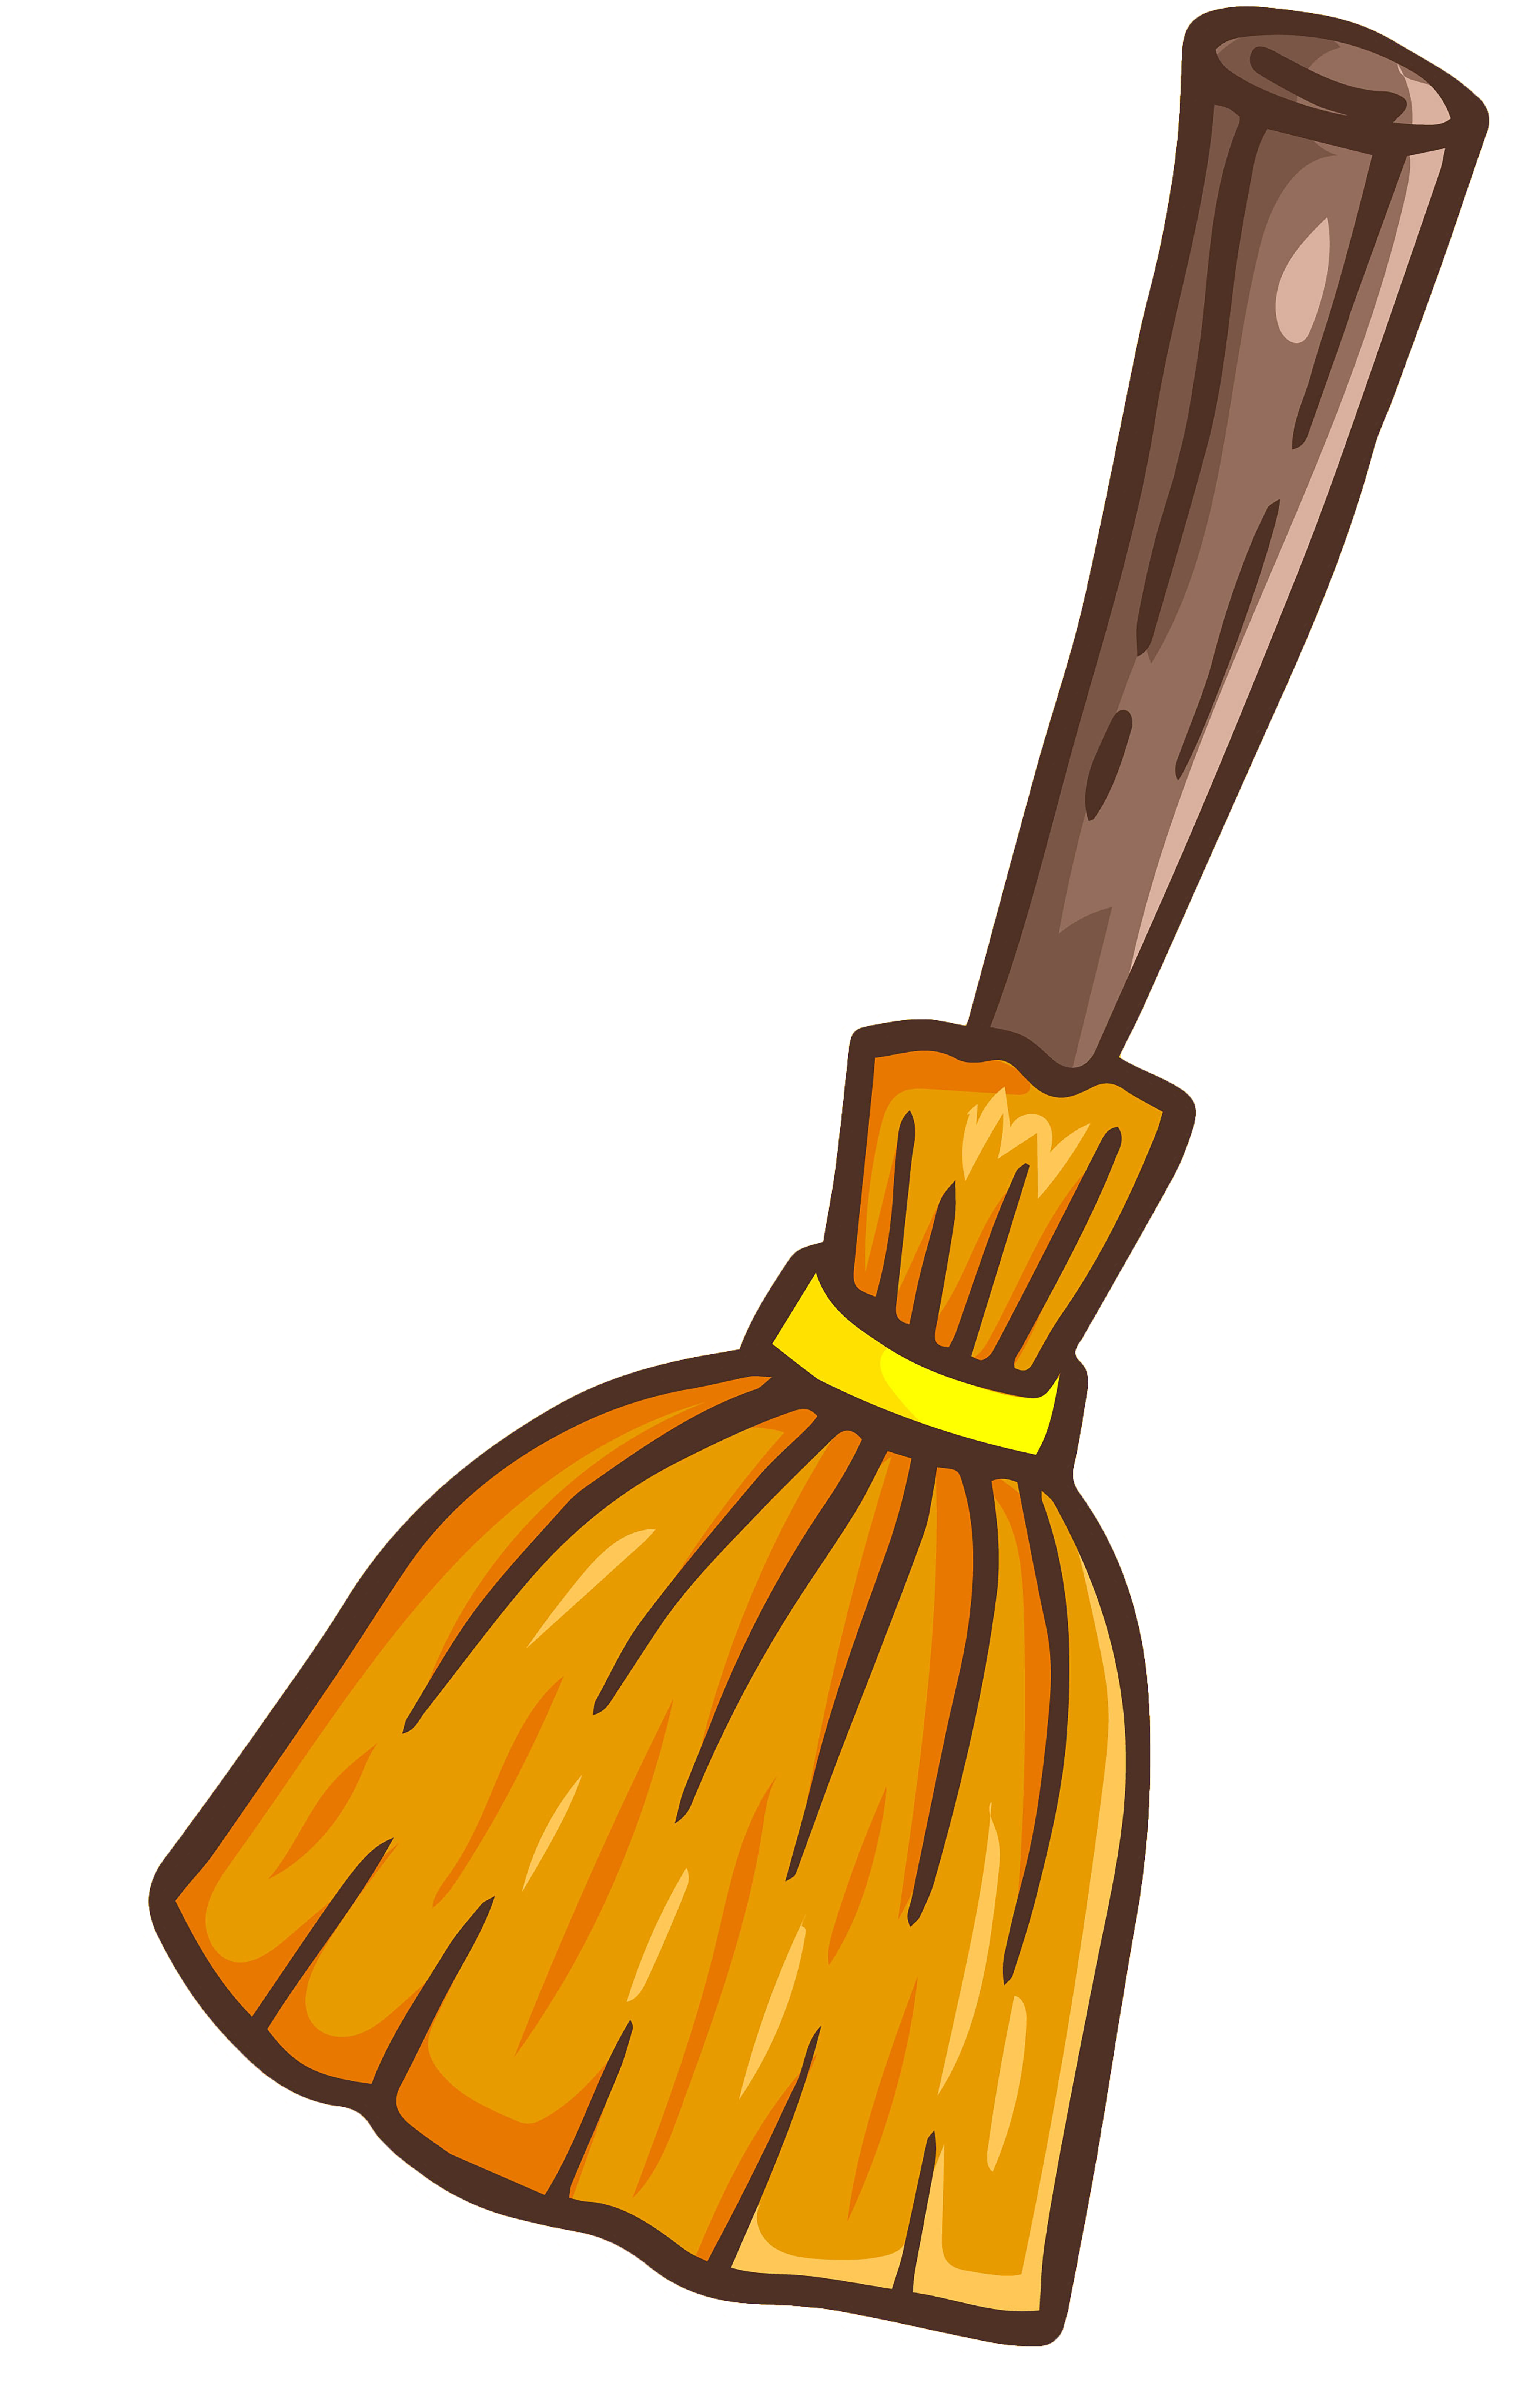
\includegraphics[width=.35\textwidth]{media/image10.png}} \\
\multicolumn{1}{c}{\textbf{\reduline{V} ELA}} & \multicolumn{1}{c}{\textbf{\reduline{V} ASSOURA}}
\end{tabular}
\end{table}

% \hspace{4cm} \reduline{F} OGO \hspace{3cm} \reduline{F} IVELA

% \begin{figure}[htpb!]
% 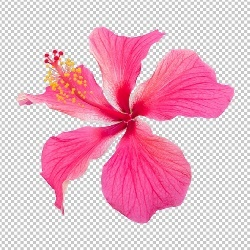
\includegraphics[width=.3\textwidth]{media/image13.jpeg}
% 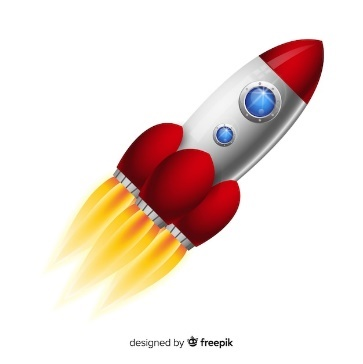
\includegraphics[width=.3\textwidth]{media/image14.jpeg}
% 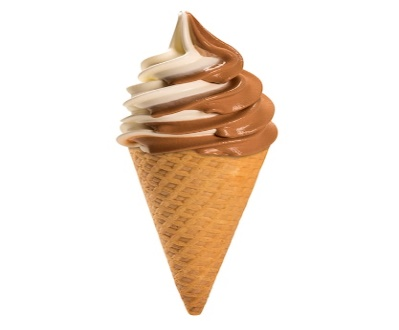
\includegraphics[width=.3\textwidth]{media/image15.jpeg}
% \end{figure}

% \reduline{F} LOR \hspace{4cm} \reduline{F} OGUETE \hspace{3cm} SOR \reduline{V} ETE


\num{5} Pinte as iniciais de cada palavra.

%\coment{Leve para sala palavras iniciadas pelas letras T, D, F, V, B, P. Convide as crianças para fazer a leitura, identificado o som das letras iniciais e finais, e quantidade de sílabas. Também é possível trabalhar a função social da escrita das palavras}.

\begin{center}
\begin{tabular}{|c|c|c|c|c|}
\hline
\textbf{-ACINA} & F & T & D & \rosa{V} \\ \hline
\textbf{-ESOURA} & P & D & \rosa{T} & F \\ \hline
\textbf{-ASSOURA} & B & T & \rosa{V} & F \\ \hline
\textbf{-ACA} & Z & \rosa{F} & D & T \\ \hline
\textbf{-EDO} & T & V & F & \rosa{D} \\ \hline
\textbf{-ANELA} & V & T & \rosa{P} & B \\ \hline
\textbf{-OMINÓ} & B & \rosa{D} & T & P \\ \hline
\textbf{-ONECA} & F & P & \rosa{B} & D \\ \hline
\end{tabular}
\end{center}

\num{6} Numere os desenhos conforme os números das palavras.

\vspace*{+1em}

%\coment{Faça leitura das palavras com as crianças, de modo que elas identifiquem a numeração e façam a associação correta.}

\begin{multicols}{3}
\begin{enumerate}

\item FOCA

\item TATU

\item PANELA

\item FORMIGA

\item VACA

\item BONECA
\end{enumerate}
\end{multicols}

\begin{table}[H]
\centering
\begin{tabular}{lll}
\reduline{(6)}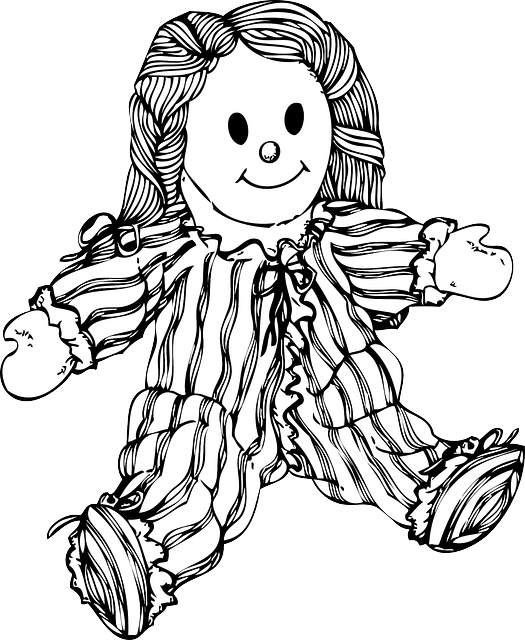
\includegraphics[width=.3\textwidth]{media/image16.png} & \reduline{(5)}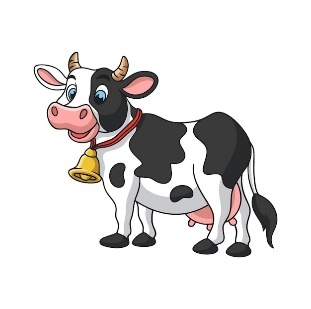
\includegraphics[width=.3\textwidth]{media/image17.jpeg} & \reduline{(5)}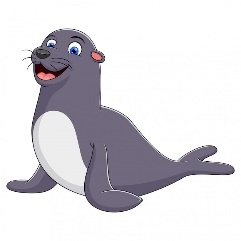
\includegraphics[width=.3\textwidth]{media/image18.jpeg}\\
\reduline{(1)}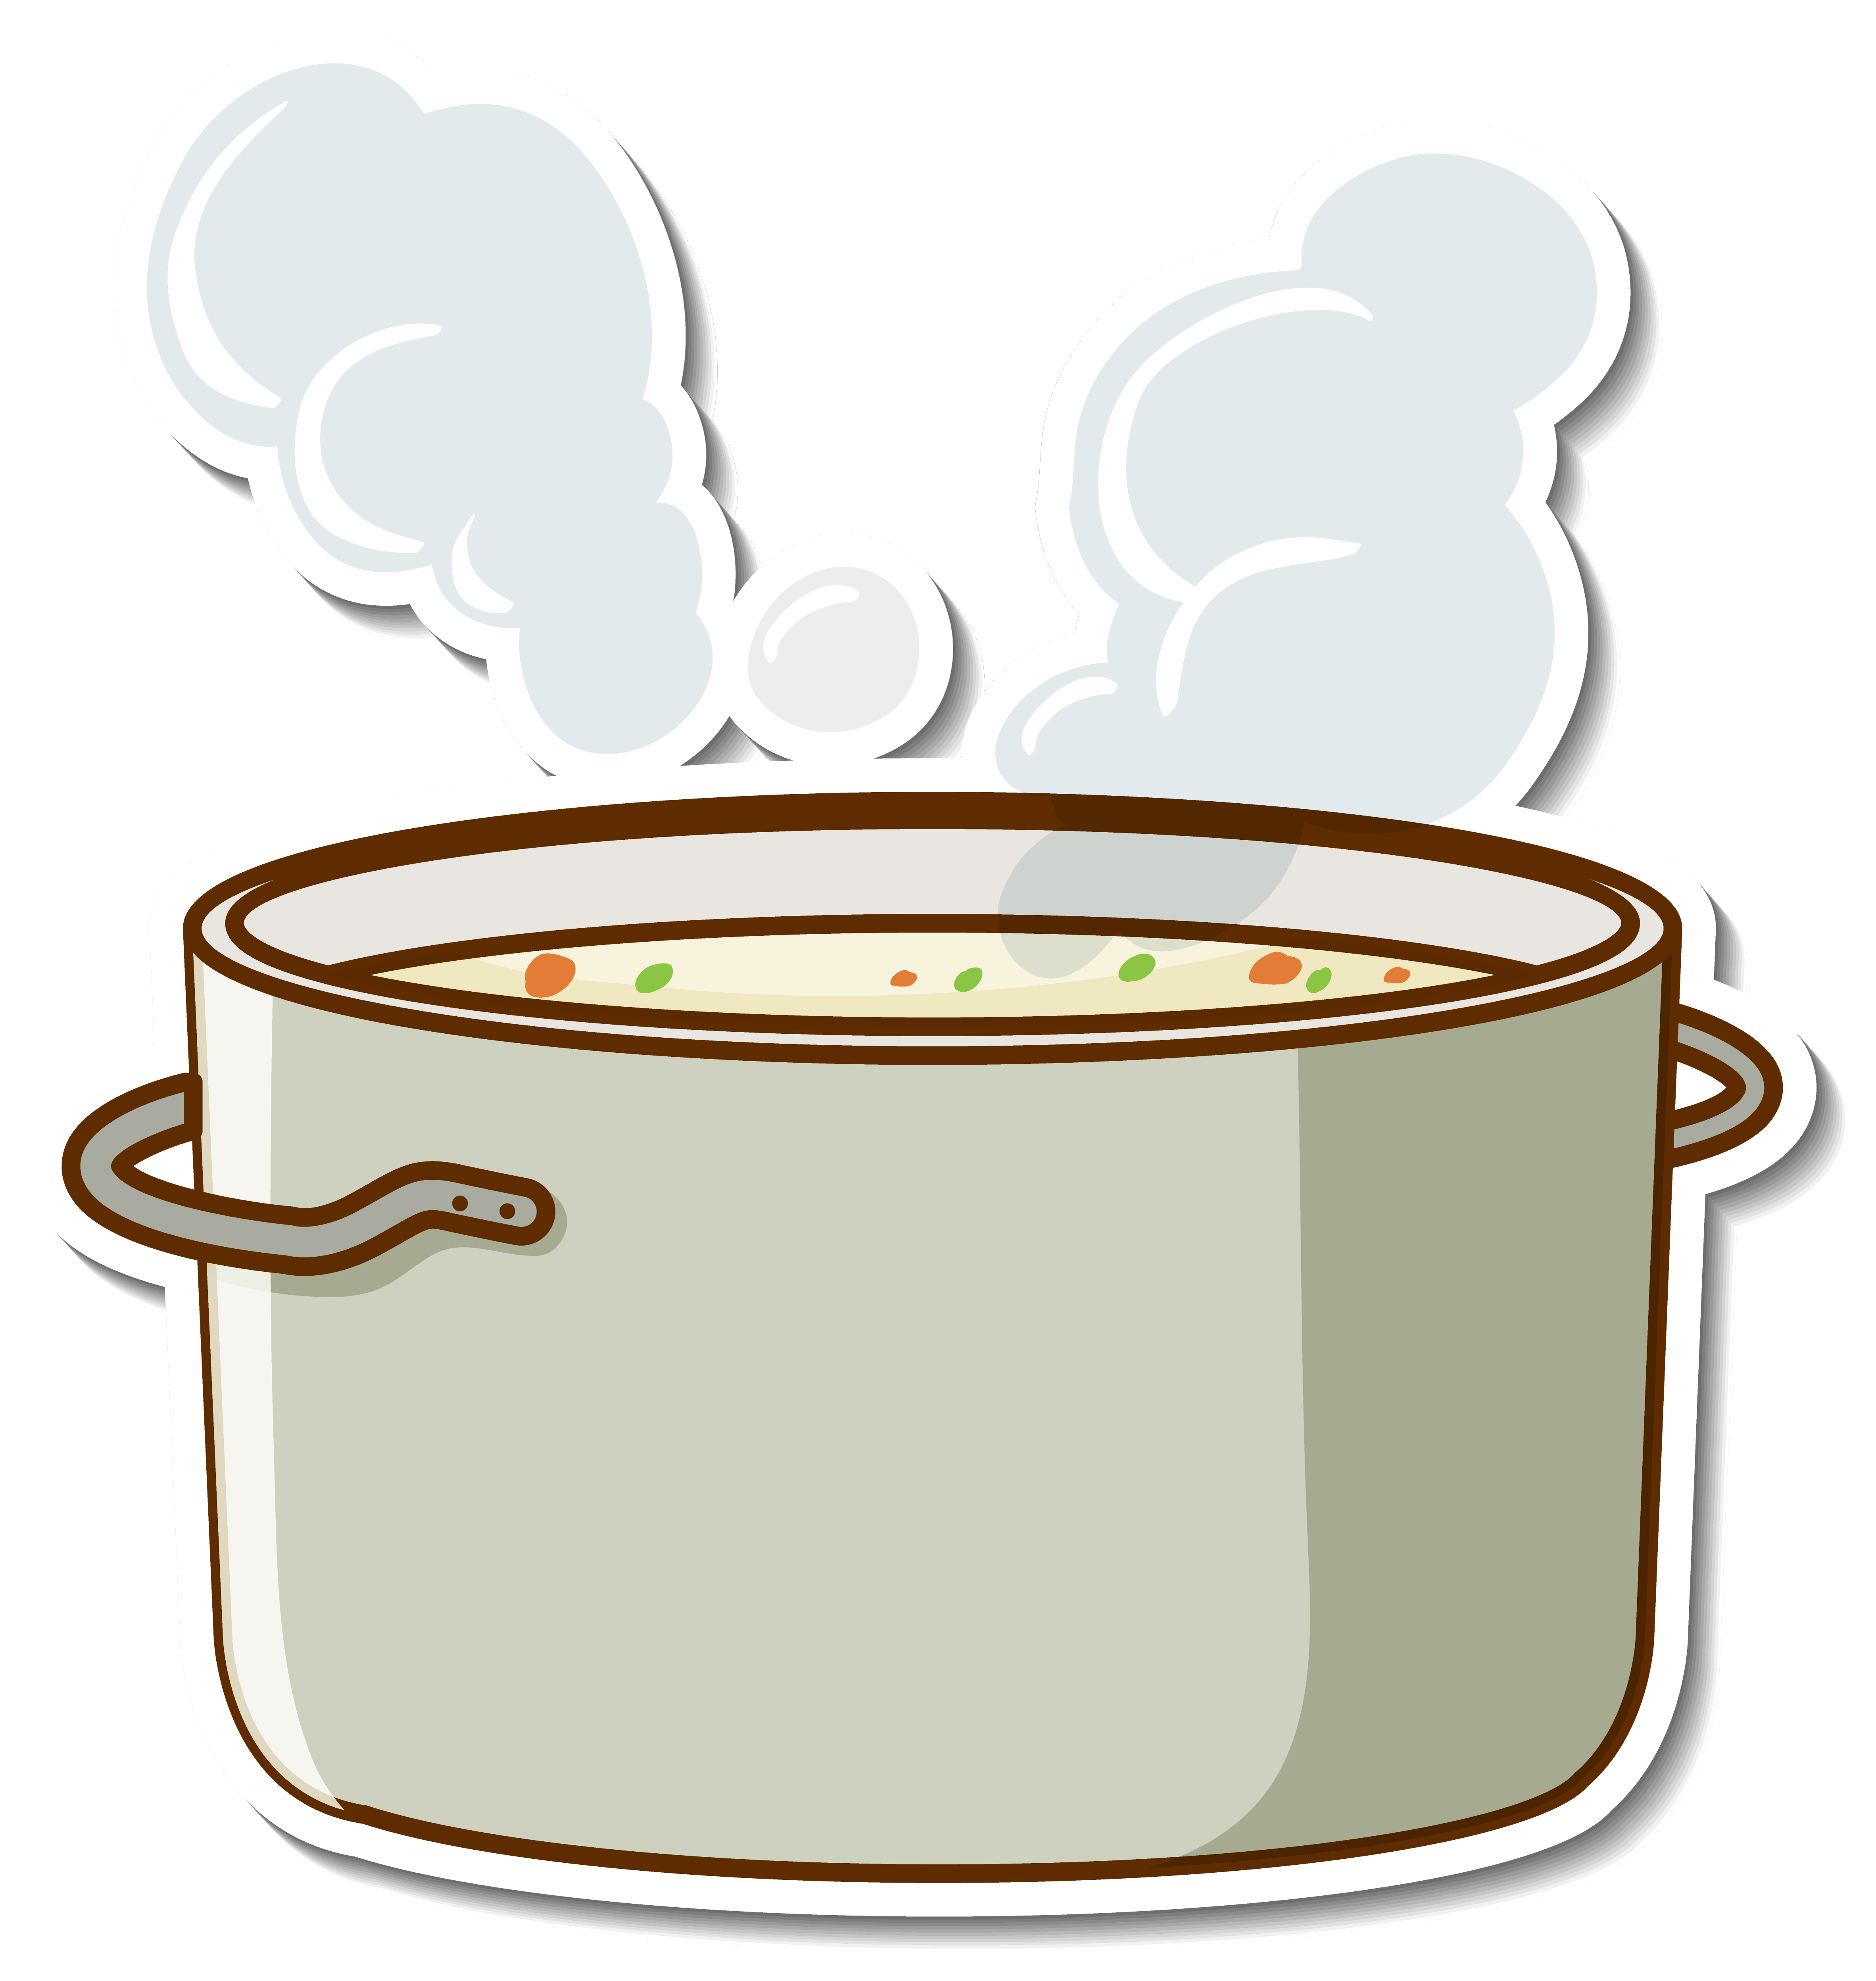
\includegraphics[width=.3\textwidth]{media/image19.jpg} & \reduline{(1)}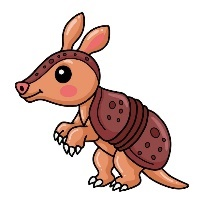
\includegraphics[width=.3\textwidth]{media/image20.jpeg} & \reduline{(3)}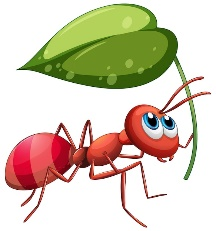
\includegraphics[width=.3\textwidth]{media/image21.jpeg}
\end{tabular}
\end{table}

\num{7} Complete as palvaras com \textbf{-ca -co -cu} ou \textbf{-qua -que -qui}.

%\coment{Convide as crianças a falar o nome das imagens para identificar a grafia da palavra.}

\begin{figure}[H]
\centering
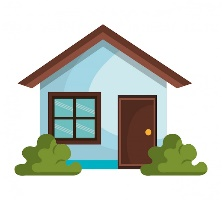
\includegraphics[width=.26\textwidth]{media/image27.jpeg}
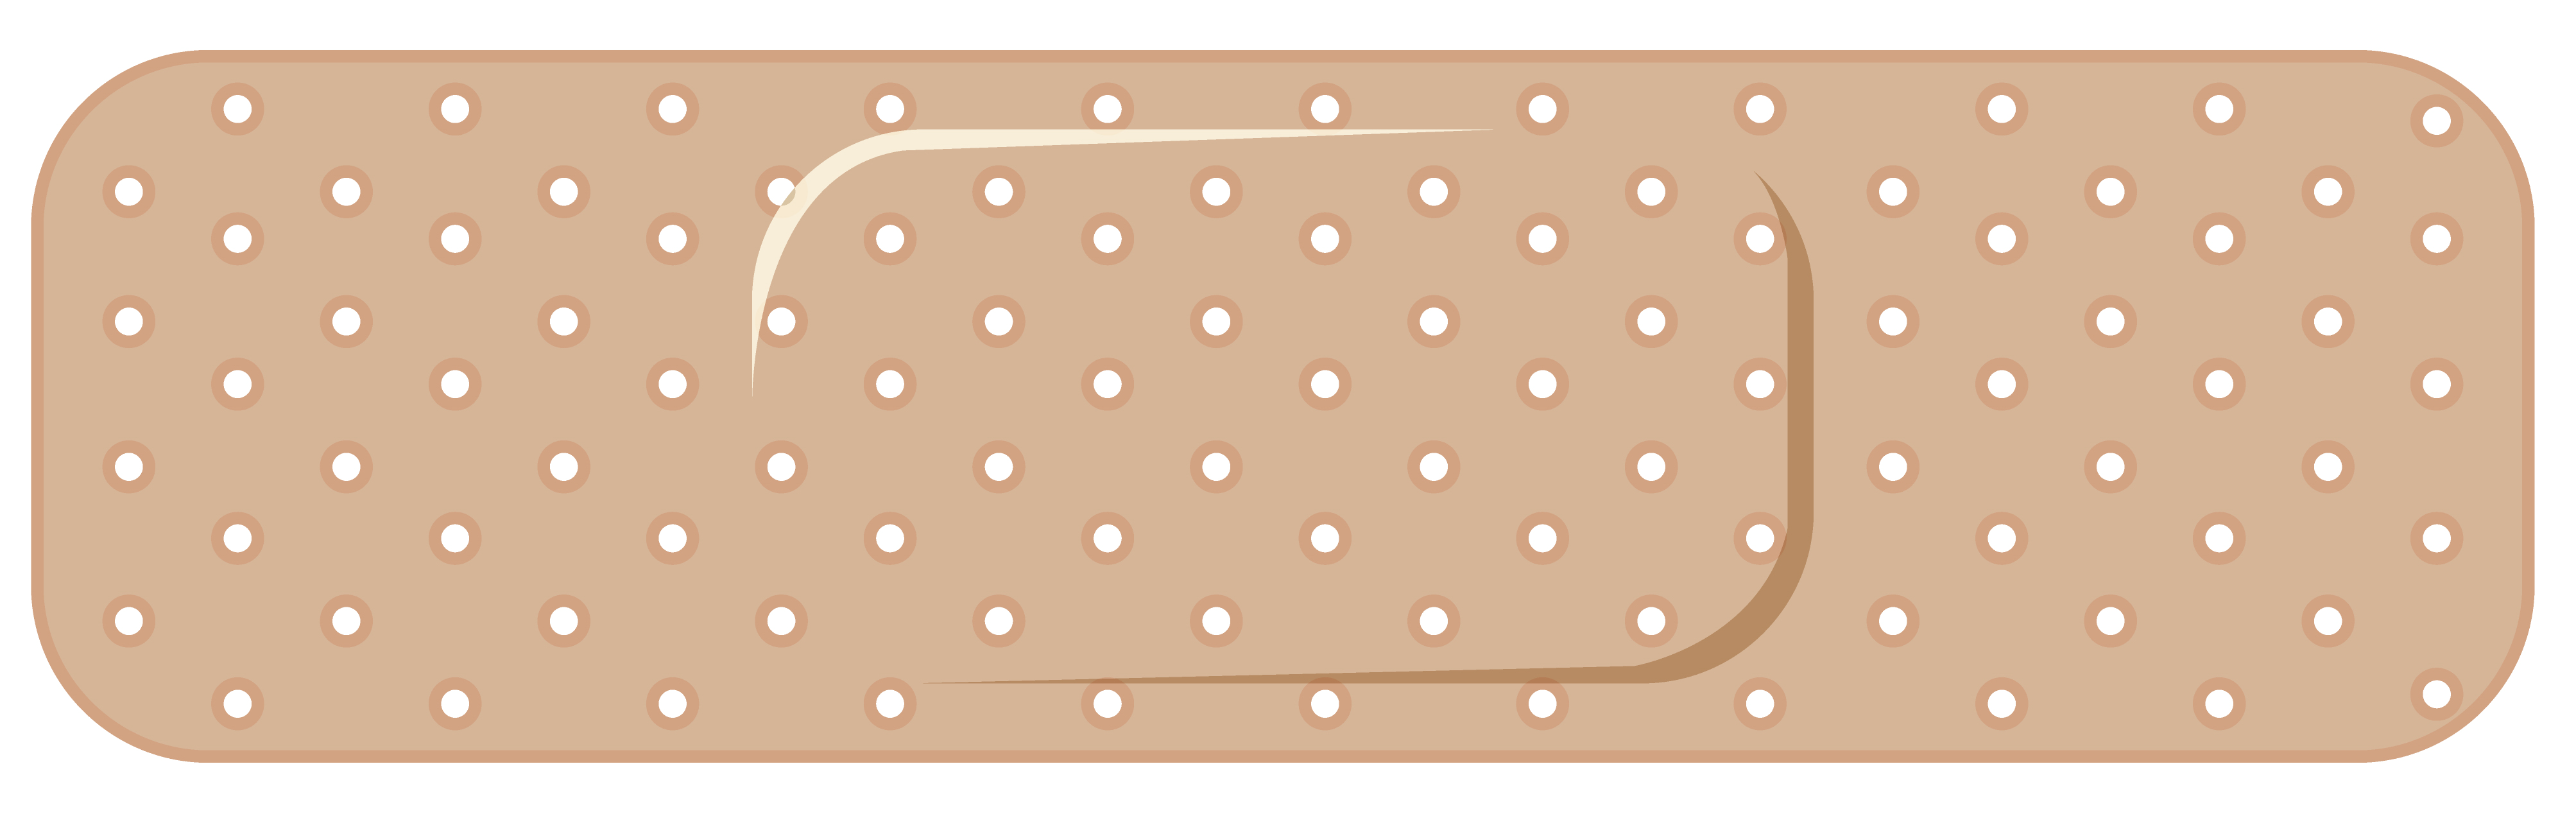
\includegraphics[width=.26\textwidth]{media/image28.png}
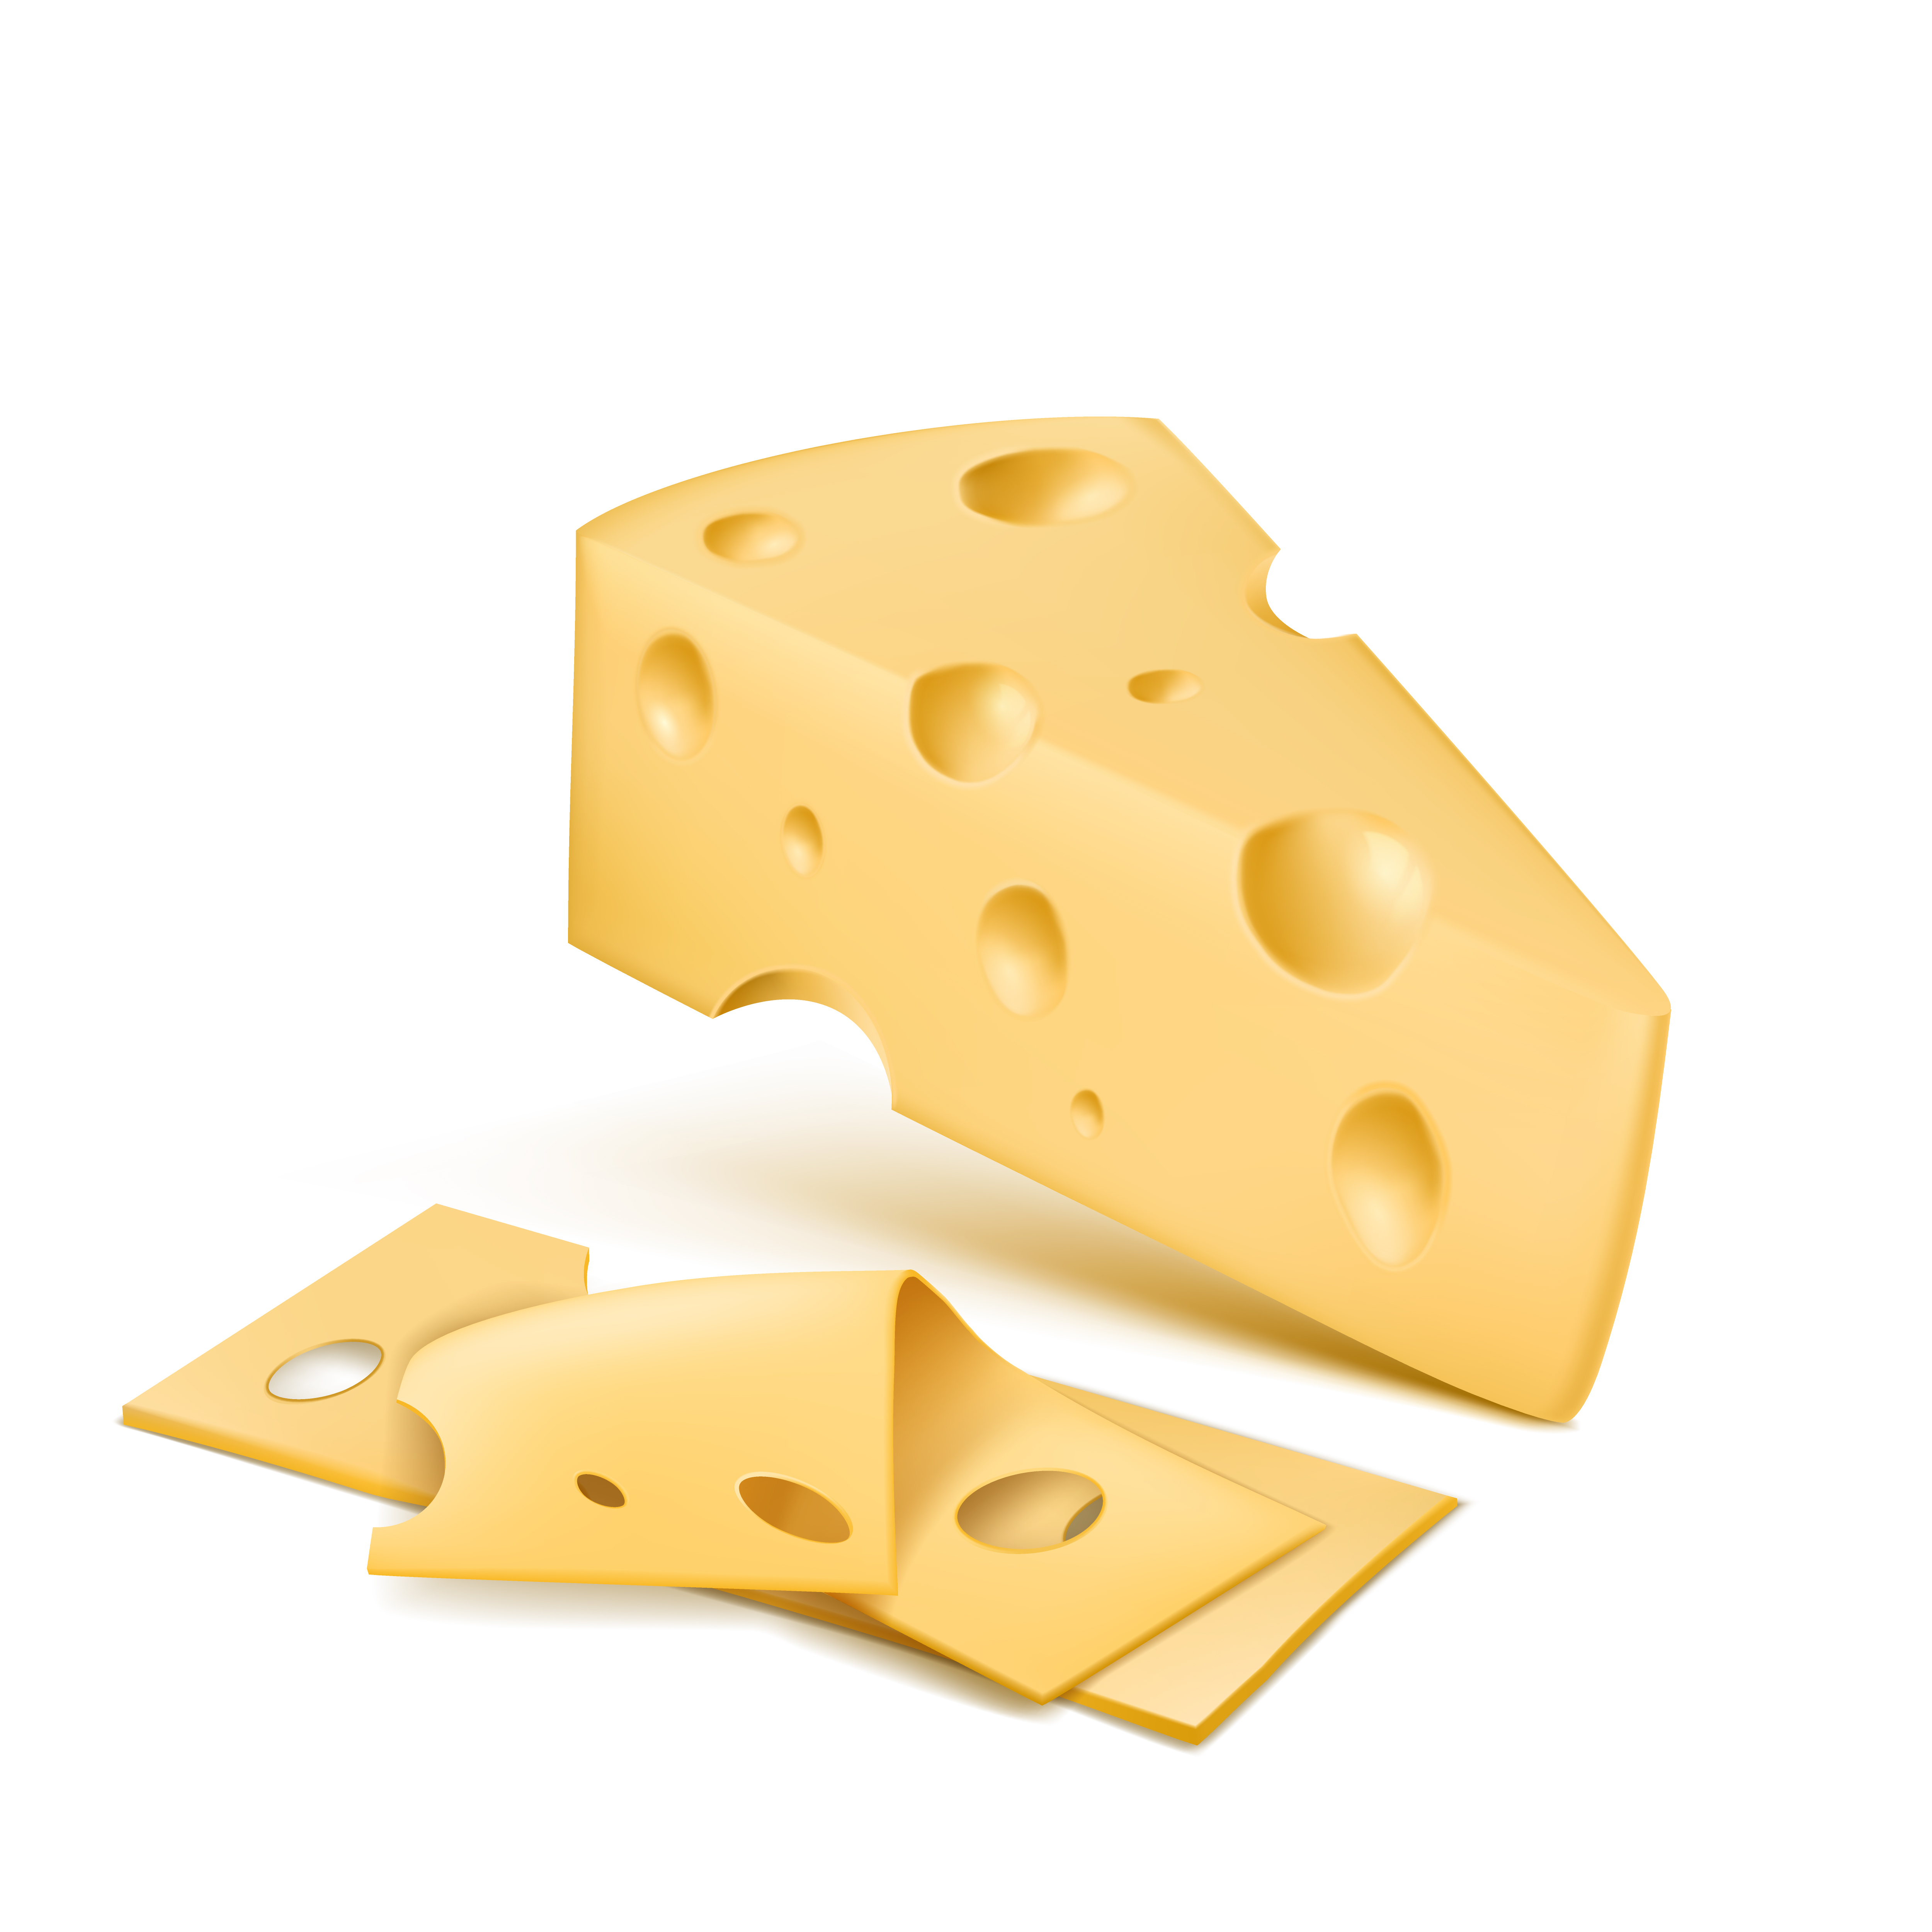
\includegraphics[width=.26\textwidth]{media/image29.jpg}
\end{figure}

\begin{center}
\reduline{CA} SA \hspace{2cm} \reduline{CU} RATIVO \hspace{2cm} \reduline{QUE} IJO
\end{center}

\vspace{-2,5em}

\begin{figure}[H]
\centering
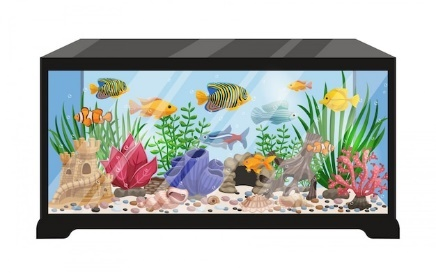
\includegraphics[width=.3\textwidth]{media/image30.jpeg}
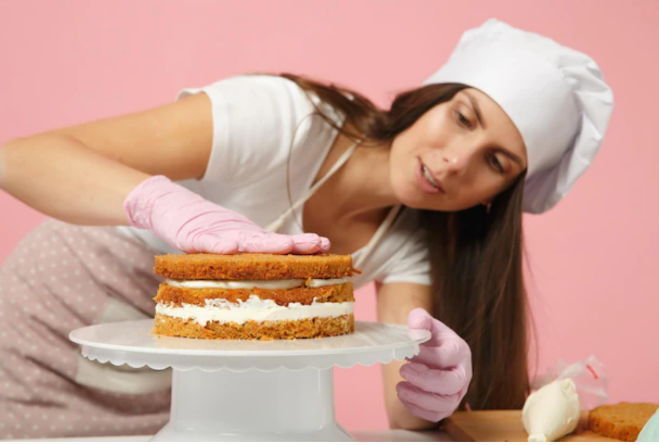
\includegraphics[width=.3\textwidth]{media/image32.png}
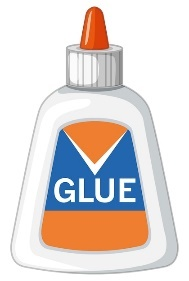
\includegraphics[width=.2\textwidth]{media/image33.jpeg}
\end{figure}

\begin{center}
A \reduline{QUÁ} RIO \hspace{2cm} RA \reduline{QUE} TE \hspace{2cm} \reduline{CO} LA
\end{center}

\num{8} Complete a sílaba mais forte das palavras com O ou U.

\vspace*{+2em}

%\coment{Leve para a classe uma caixinha enfeitada com palavras terminadas com O e U. Passe a caixinha para os alunos em círculo, ao som de uma música. Quando a música parar, o aluno que estiver com a caixinha na mão deve ler a palavra observando a letra  final. Em seguida, convide toda a turma a pronunciar a palavra e, então, descobrir a sílaba forte. Explique como descobrir quando a sílaba é forte e fraca, ensinando que, quando o U está no final, ele é sempre forte, e que o O é sempre fraco no final das palavras.}

SAPAT \reduline{O} \hspace{1cm} VAS \reduline{O} \hspace{2cm} TAT \reduline{U}
\vspace{-1em}

ESPELH \reduline{O} \hspace{1cm} CAJ \reduline{U} \hspace{2cm} CABEL \reduline{O}

\num{9} Pinte as palavras escritas com C, mas com som de S.

\vspace*{+1em}
%Felipe: aqui precisamos padronizar, como comentei anteriormente. 

%\coment{Leve para sala palavras escritas com C. Organize uma roda de conversa na qual você orientará os alunos a organizar as palavras de acordo com a vogal que acompanha a letra C. Em seguida, explique a regra para descobrir se o C tem som de K ou S.}

\begin{longtable}[]{@{}lllll@{}}
\toprule
\textbf{CINEMA} & \textbf{CASA} & \textbf{CISNE} & \textbf{CEGO} &
\textbf{COCADA}\tabularnewline
\midrule
\endhead
\textbf{CADEIRA} & \textbf{CARRO} & \textbf{CINTO } & \textbf{COCO} &
\textbf{CAMA}\tabularnewline
\bottomrule
\end{longtable}

\num{10} Troque as letras e forme outras palavras.

%\coment{Utilize o alfabeto móvel com as palavras solicitadas no exercício e outras. Também é possível fazer a brincadeira da forca.}

\begin{table}[H]
\centering
\begin{tabular}{ccc}
\hline
\textbf{V por F} & \textbf{D por T} & \textbf{B por P} \\ \hline
\textbf{VACA}    & \textbf{DADO}    & \textbf{BODE}    \\
\textbf{\_\_ACA} & \textbf{\_\_ATO} & \textbf{\_\_ODE} \\
\textbf{VILA}    & \textbf{DIA}     & \textbf{BOTE}    \\
\textbf{\_\_ILA} & \textbf{\_\_IA}  & \textbf{\_\_OTE} \\ \hline
\end{tabular}
\end{table}

% \pagebreak
% \num{11} Complete a cruzadinha com o nome das figuras.

% %\coment{Explore as frutas e legumes da atividade, fazendo questionamentos. Monte as palavras no alfabeto móvel com as crianças. Em seguida, oriente a escrita na cruzadinha.}

% \begin{figure}[htpb!]
% 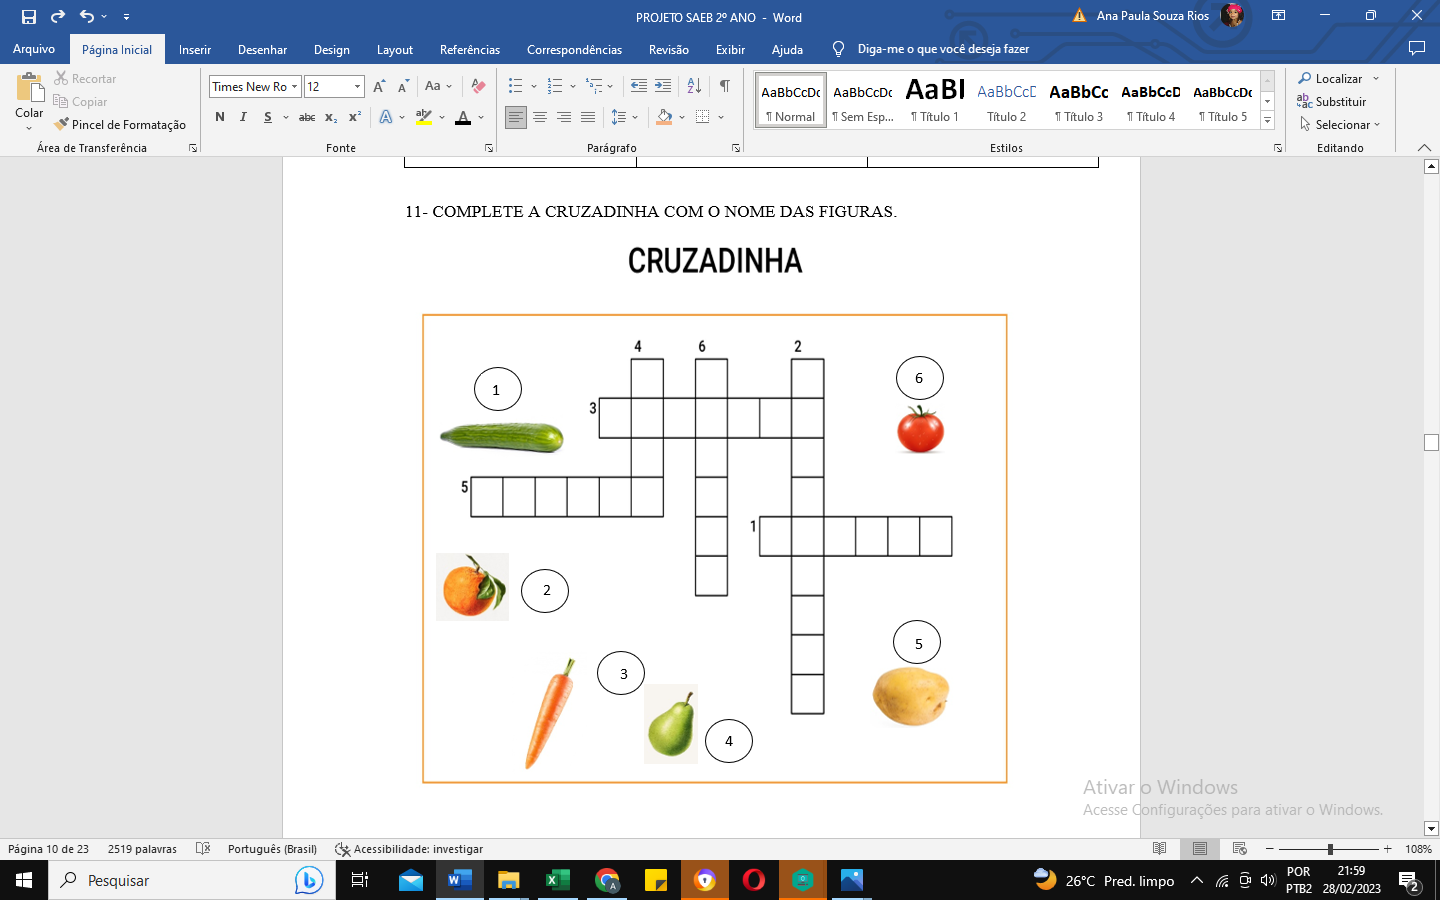
\includegraphics[width=\textwidth]{media/image40.png}
% \end{figure}

% \num{12} Encontre e pinte as palavras no diagrama.

% %\coment{Depois da leitura das palavras, oriente os alunos a localizá-las no diagrama.}

% \begin{longtable}[]{@{}llllllll@{}}
% \toprule
% 	TATU -- CABELO -- BONECA -- PANELA -- CAJU\tabularnewline
% FADA -- DADO -- VASO -- CAMA -- TAPETE\tabularnewline
% \midrule
% D & B & F & A & D & A & D & G\tabularnewline
% A & C & A & B & E & L & O & U\tabularnewline
% G & Y & B & O & C & A & M & A\tabularnewline
% S & T & I & N & H & M & A & Q\tabularnewline
% P & A & N & E & L & A & D & F\tabularnewline
% H & T & O & C & A & J & U & L\tabularnewline
% J & U & K & A & D & A & D & O\tabularnewline
% T & A & P & E & T & E & Z & X\tabularnewline
% K & V & A & S & O & B & G & J\tabularnewline
% \end{longtable}

\section*{Treino}

\num{1} Observe o animal que Júlia encontrou enquanto brincava na 
fazenda do Tio Belo.

\begin{figure}[htpb!]
\centering

\includegraphics[width=\textwidth]{media/image42.jpeg}
\end{figure}

A palavra que apresenta o mesmo som inicial do nome desse animal é

\begin{escolha}[itemsep=-3pt]
\item vaso.

\item gato.

\item bola.

\item foca.
\end{escolha}

\pagebreak
\num{2} Observe a palavra que Tiago leu para sua professora.

\begin{myquote}
\centering
CAJU
\end{myquote}

A palavra que termina com a mesma letra do termo acima é

\begin{escolha}[itemsep=-3pt]
\item\ cabelo.

\item\ sapato.

\item\ relógio.

\item\ canguru.
\end{escolha}


\num{3} Observe o presente que Bruna ganhou.

\begin{figure}[H]
\centering
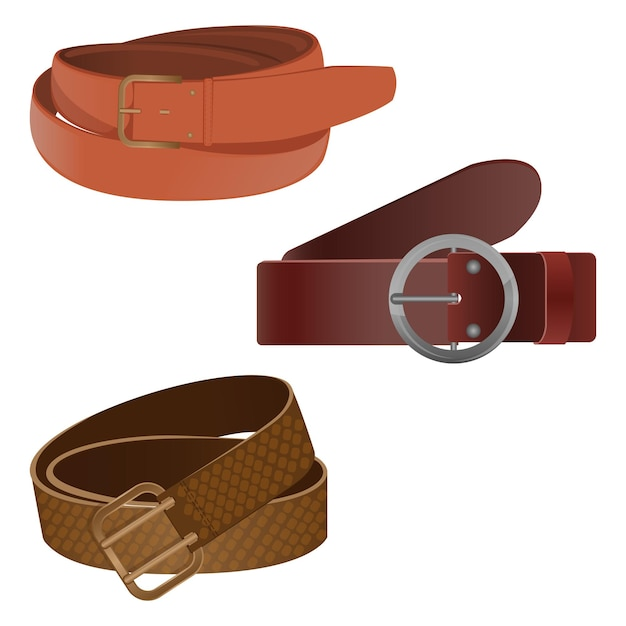
\includegraphics[width=.5\textwidth]{media/image48.jpeg}
\end{figure}

A palavra que começa como o mesmo som da letra do nome do presente de Bruna é

\begin{escolha}[itemsep=-3pt]
\item cama.

\item cubo.

\item cebola.

\item cocada.
\end{escolha}

\chapter{Lendo e escrevendo}
\markboth{Módulo 2}{}

\vspace*{-1cm}

\section*{Habilidades do SAEB}

\begin{itemize}
\item Ler palavras.
\item Escrever palavras.
\item Ler frases.
\end{itemize}

\subsection{Habilidades da BNCC}

\begin{itemize}
\item EF02LP04, EF02LP05.
\end{itemize}

\conteudo{Para escrever uma palavra, você precisa usar as letras. No último módulo, vimos que elas são divididas em \textbf{vogais} e \textbf{consoantes}. Você se lembra de cada grupo?

As vogais são 

\begin{myquote}
\centering
\vspace*{-1em}
\textbf{A -- E -- I -- O -- U} 
\end{myquote}

e as consoantes são

\begin{myquote}
\centering
\vspace*{-1em}
\textbf{B -- C -- D -- F -- G -- H -- J -- K -- L -- M -- N -- P -- Q -- R -- S
-- T -- V -- W -- Y -- X -- Z.}
\end{myquote}

As palavras são lidas e escritas da esquerda para a direita.

\begin{myquote}
\centering
\vspace*{-1em}
$\longrightarrow$\\
\textbf{GRAVIOLA LÂMPADA AVIÃO LARANJA }
\end{myquote}

Existem diferentes maneiras de formar a sílaba de uma palavra. 

\textbf{CONSOANTE + VOGAL}: é o que acontece nas três sílabas das 
palavras \textit{sapato} e \textit{telefone}: SA-PA-TO e TE-LE-FO-NE

\textbf{VOGAL}: é o que acontece na segunda sílaba das  
palavras \textit{saída} e \textit{saúde}: SA-Í-DA e SA-Ú-DE

\textbf{CONSOANTE + VOGAL + CONSOANTE}: é o que acontece na 
primera sílaba das palavras \textit{porta} e \textit{cortina}:
POR-TA e COR-TI-NA

\textbf{CONSOANTE + CONSOANTE + VOGAL}: é o que acontece na 
primera sílaba da palavra \textit{criança} e na última
sílaba da palavra \textit{livro}: CRI-AN-ÇA e LI-VRO 

Note que, em todas as formações das sílabas, aparecem vogais. Isso
acontece porque não existe sílaba sem vogal, isto é, uma  sílaba não
se forma só com consoantes.

Observe a frase a seguir:

\begin{myquote}
\centering
\vspace*{-1em}
\textbf{O avião pousou cedo.}
\end{myquote}

Você conhece esse sinal em cima da letra A da palavra \textbf{avião}?

Esse sinal é o \textbf{til}, usado nas vogais A e O para marcar a
nasalidade presente na sílaba.

As marcas de nasalidade aparece também nas letras M e N, no final da
sílaba. É o que acontece, por exemplo, com as seguintes palavras:

\begin{myquote}
\centering
\vspace*{-1em}
\textbf{LÂMPADA E LARANJA}
\end{myquote}

A letra \textbf{M} é utilizada antes das consoantes P e B.  
A letra \textbf{N} é usada antes das demais consoantes, nunca 
no final das palavras.
}

\section*{Atividades}

\num{1} Separe as sílabas das palavras, depois circule as sílabas formadas por
consoante + consoante + vogal.

%\coment{Leia as palavras com os alunos, orientando-os a identificar vogais e consoantes. Também é possível montar algumas palavras com o alfabeto móvel. Em seguida, peça a eles que batam palmas cada vez que um pedacinho da palavra for pronunciado.}

\begin{longtable}[]{@{}ll@{}}
\toprule
\textbf{PRATO} & \rosa{Pra - to}\tabularnewline
\midrule
\textbf{FORMIGA} & \rosa{For- mi -ga}\tabularnewline
\midrule
\textbf{BRAÇO} & \rosa{Bra -ço}\tabularnewline
\midrule
\textbf{DRAGÃO} & \rosa{Dra- gão}\tabularnewline
\midrule
\textbf{CRAVO} & \rosa{Cra -- vo}\tabularnewline
\bottomrule
\end{longtable}

\pagebreak

\num{2} Escreva os nomes das figuras.

%\coment{Leve o alfabeto móvel para a sala de aula. Convide as crianças para manusear as letras; em seguida, oriente-as a formar as palavras que nomeiam as figuras. Sugira a elas que, antes de escrever, elas devem pronunciar a palavra, escrevendo-a por sílabas ou pedacinhos.}

\begin{figure}[H]
\centering
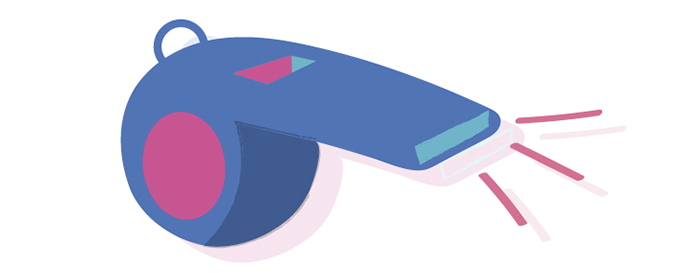
\includegraphics[width=.25\textwidth]{media/image49.png}
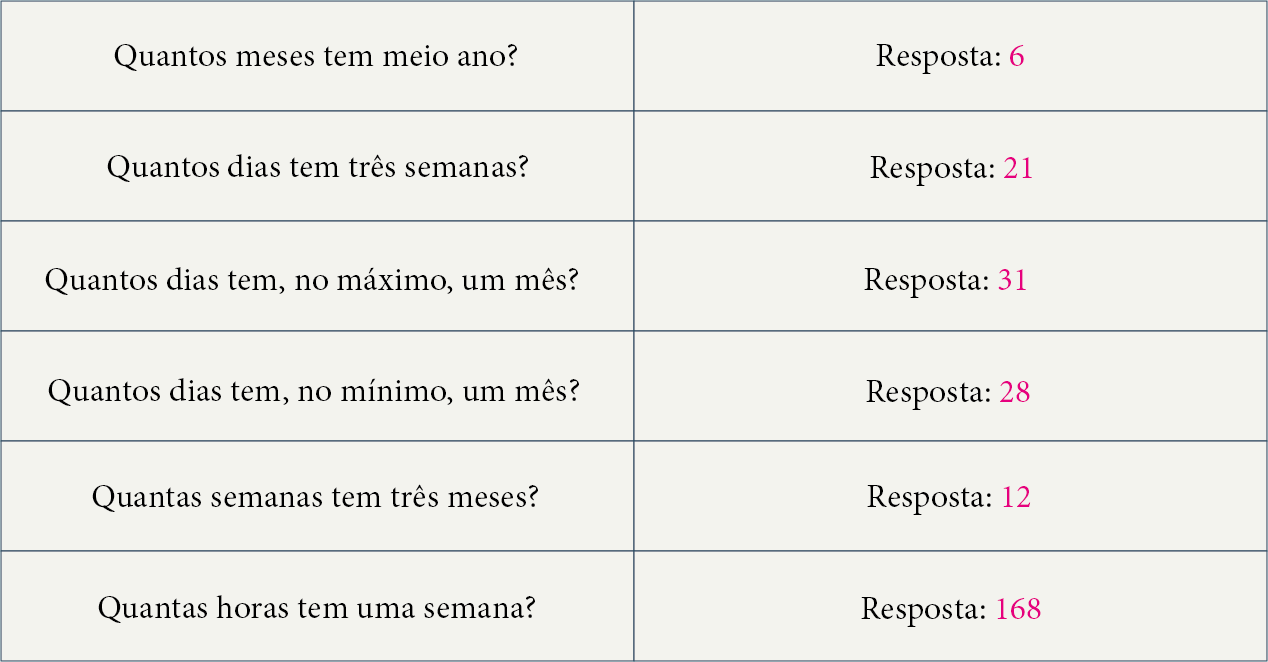
\includegraphics[width=.25\textwidth]{media/image50.png}
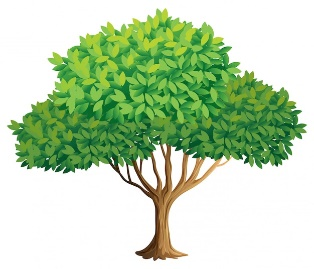
\includegraphics[width=.25\textwidth]{media/image51.jpeg}
\end{figure}

\reduline{Apito\hfill}

\reduline{Bicicleta\hfill}

\reduline{Árvore\hfill}

\vspace*{-1em}

\begin{figure}[H]
\centering
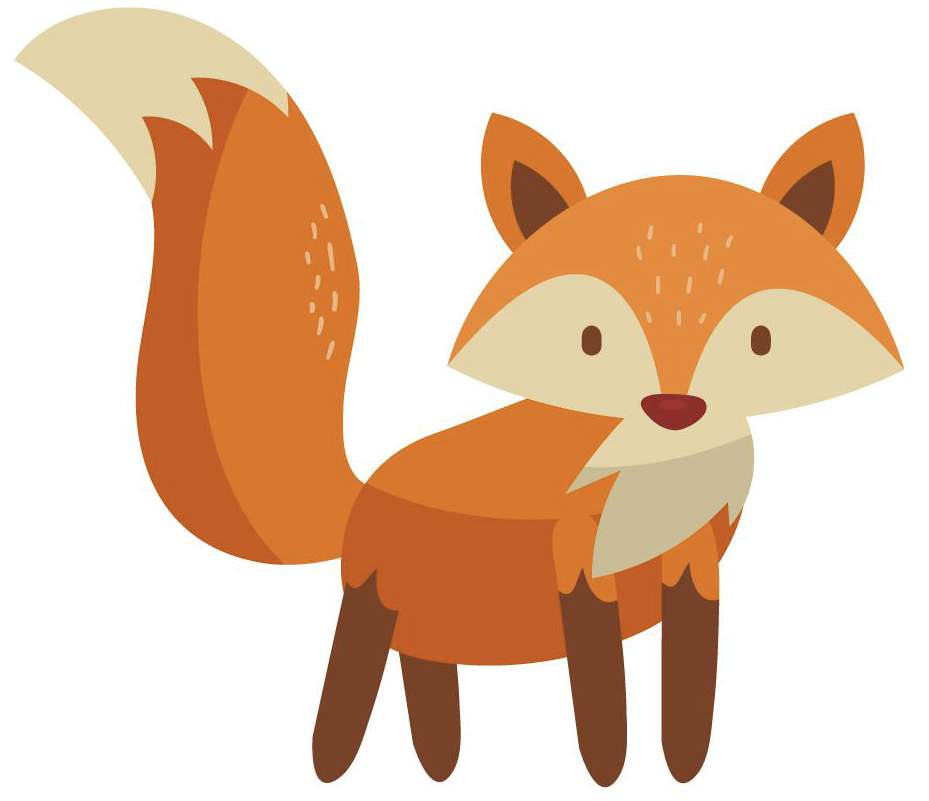
\includegraphics[width=.25\textwidth]{media/image52.png}
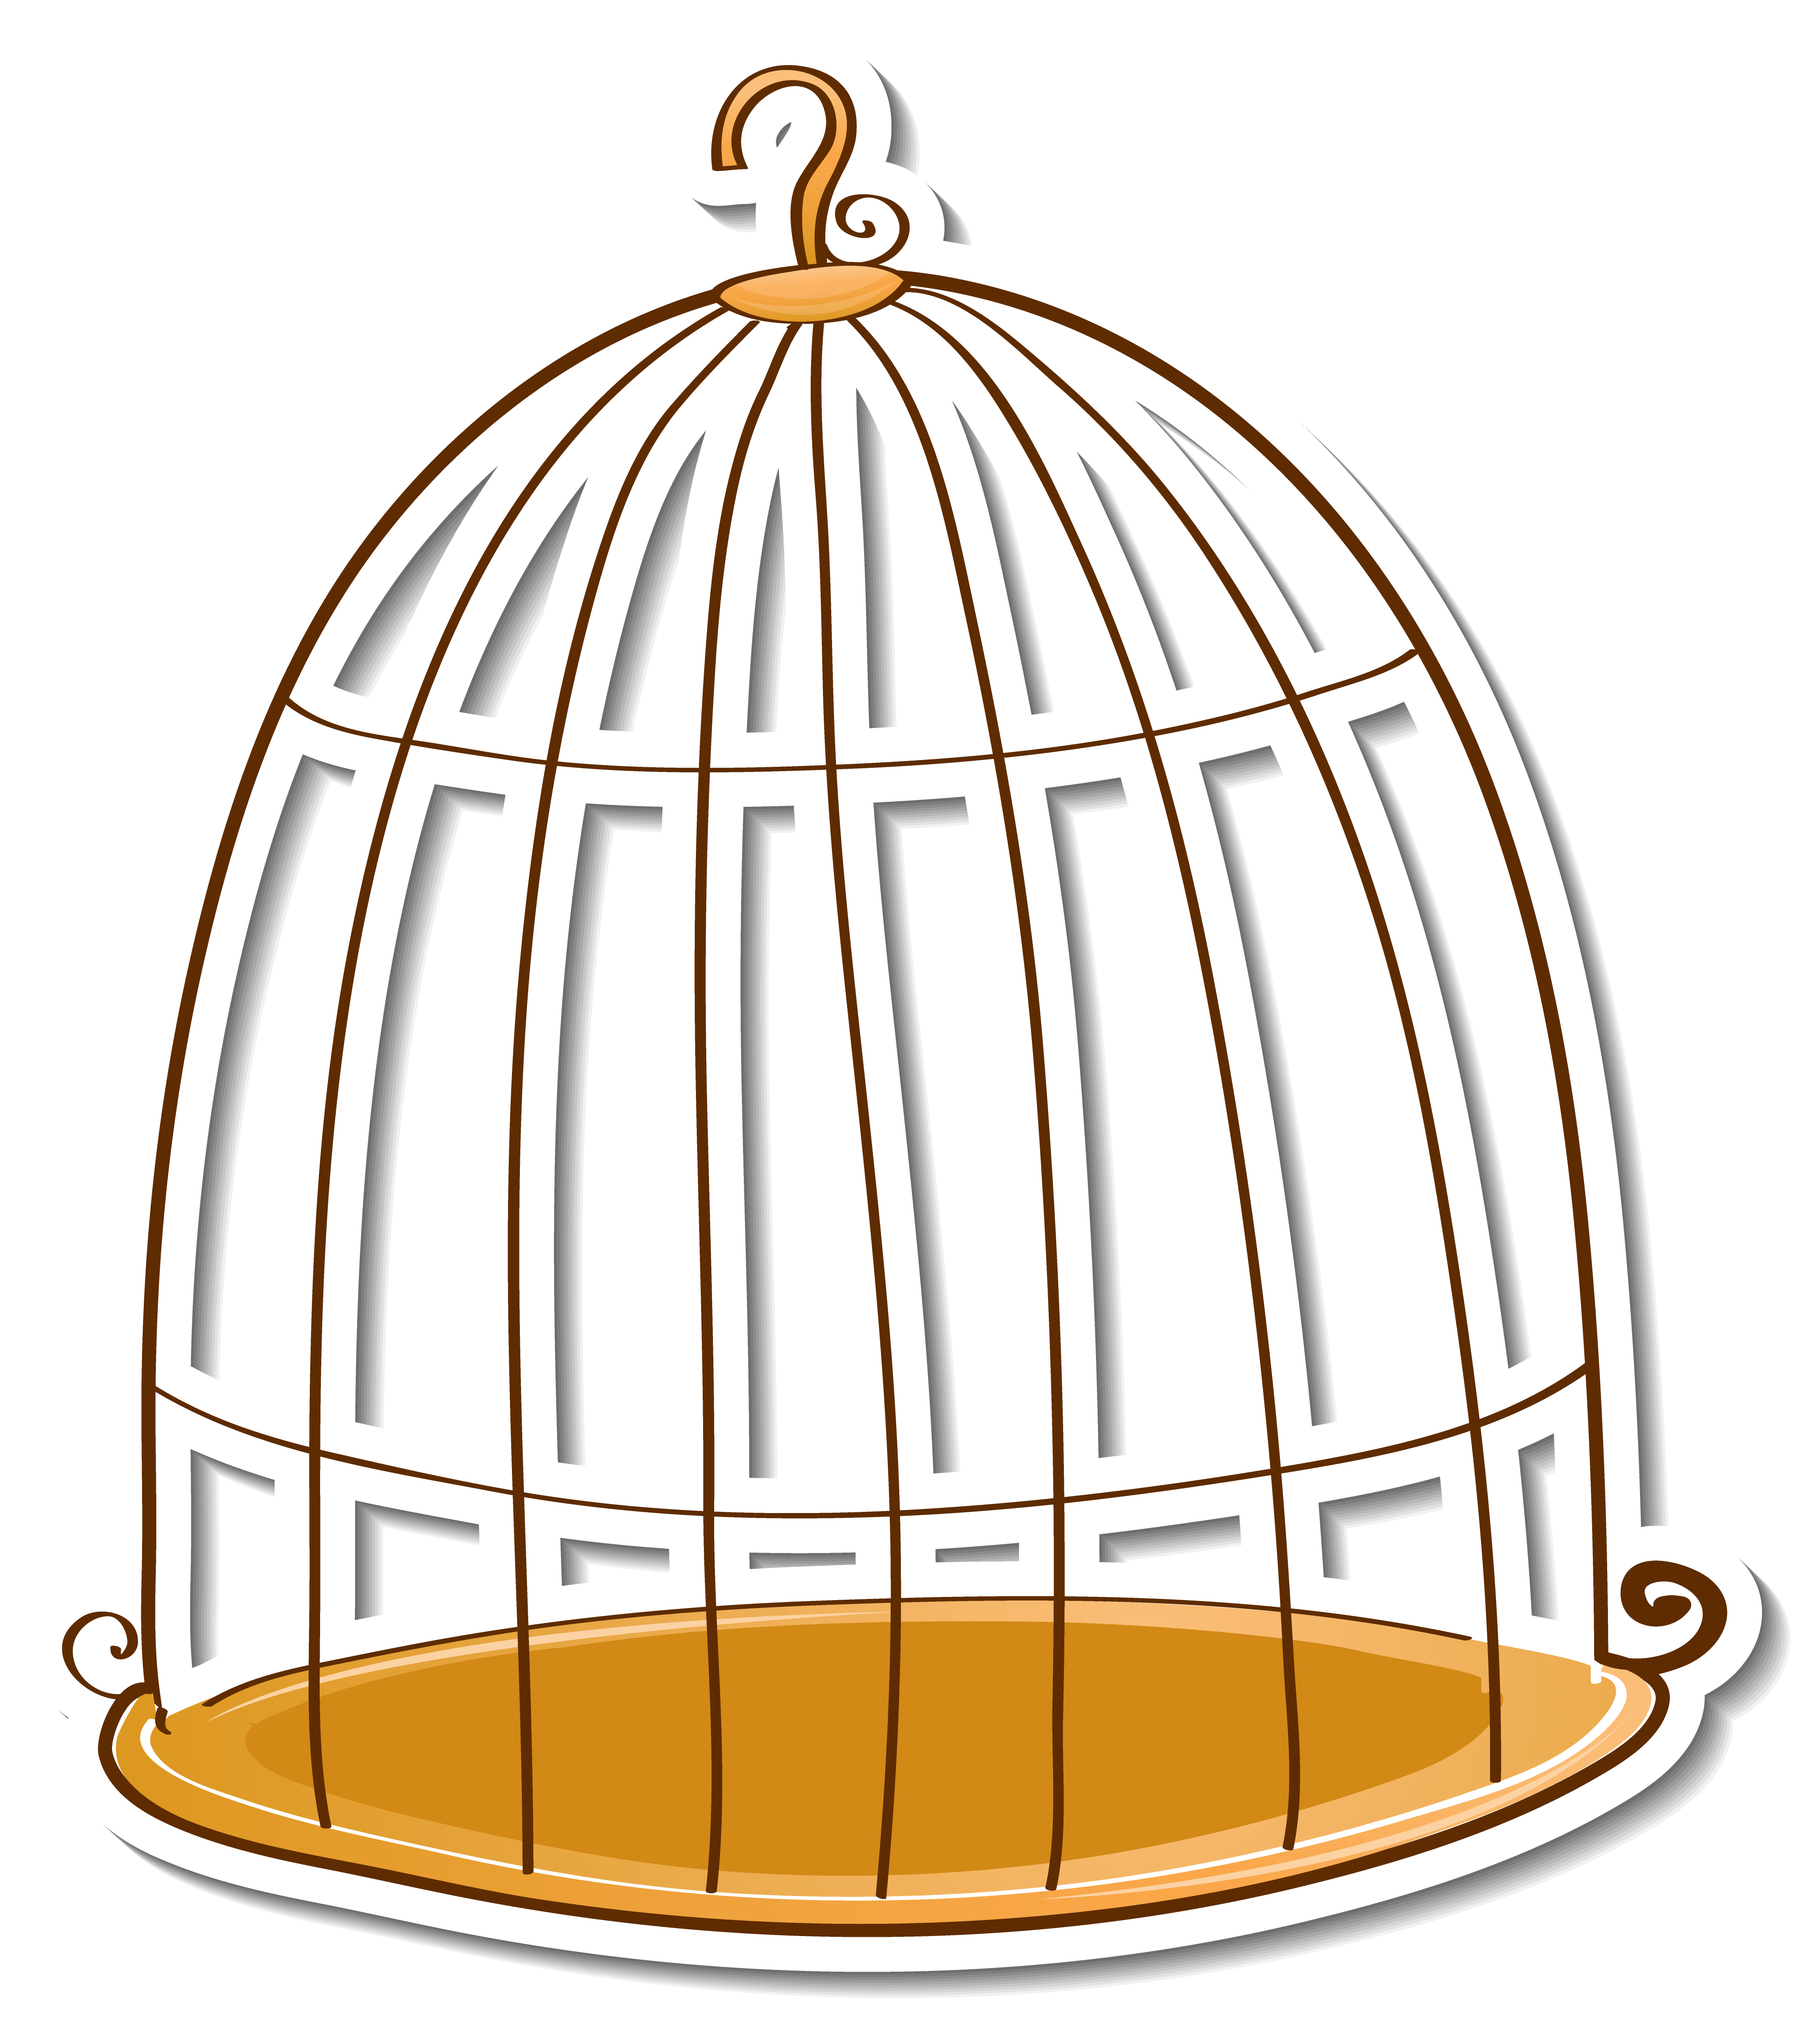
\includegraphics[width=.2\textwidth]{media/image53.jpg}
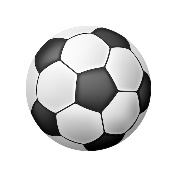
\includegraphics[width=.25\textwidth]{media/image54.jpeg}
\end{figure}

\reduline{Raposa\hfill}

\reduline{Gaiola\hfill}

\reduline{Bola\hfill}

\vspace*{-1em}

\begin{figure}[H]
\centering
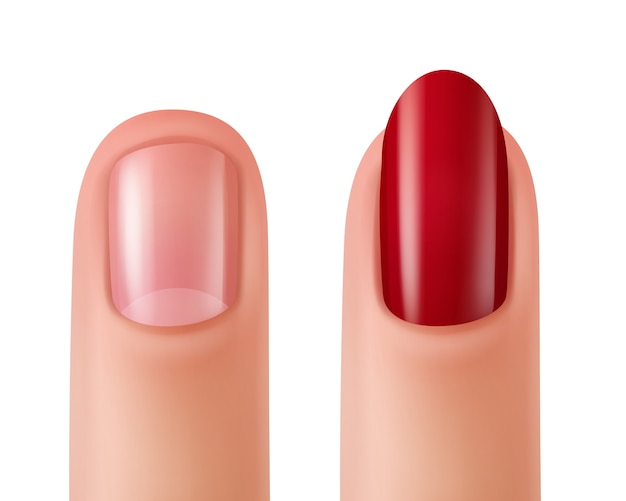
\includegraphics[width=.25\textwidth]{media/image55.jpeg}
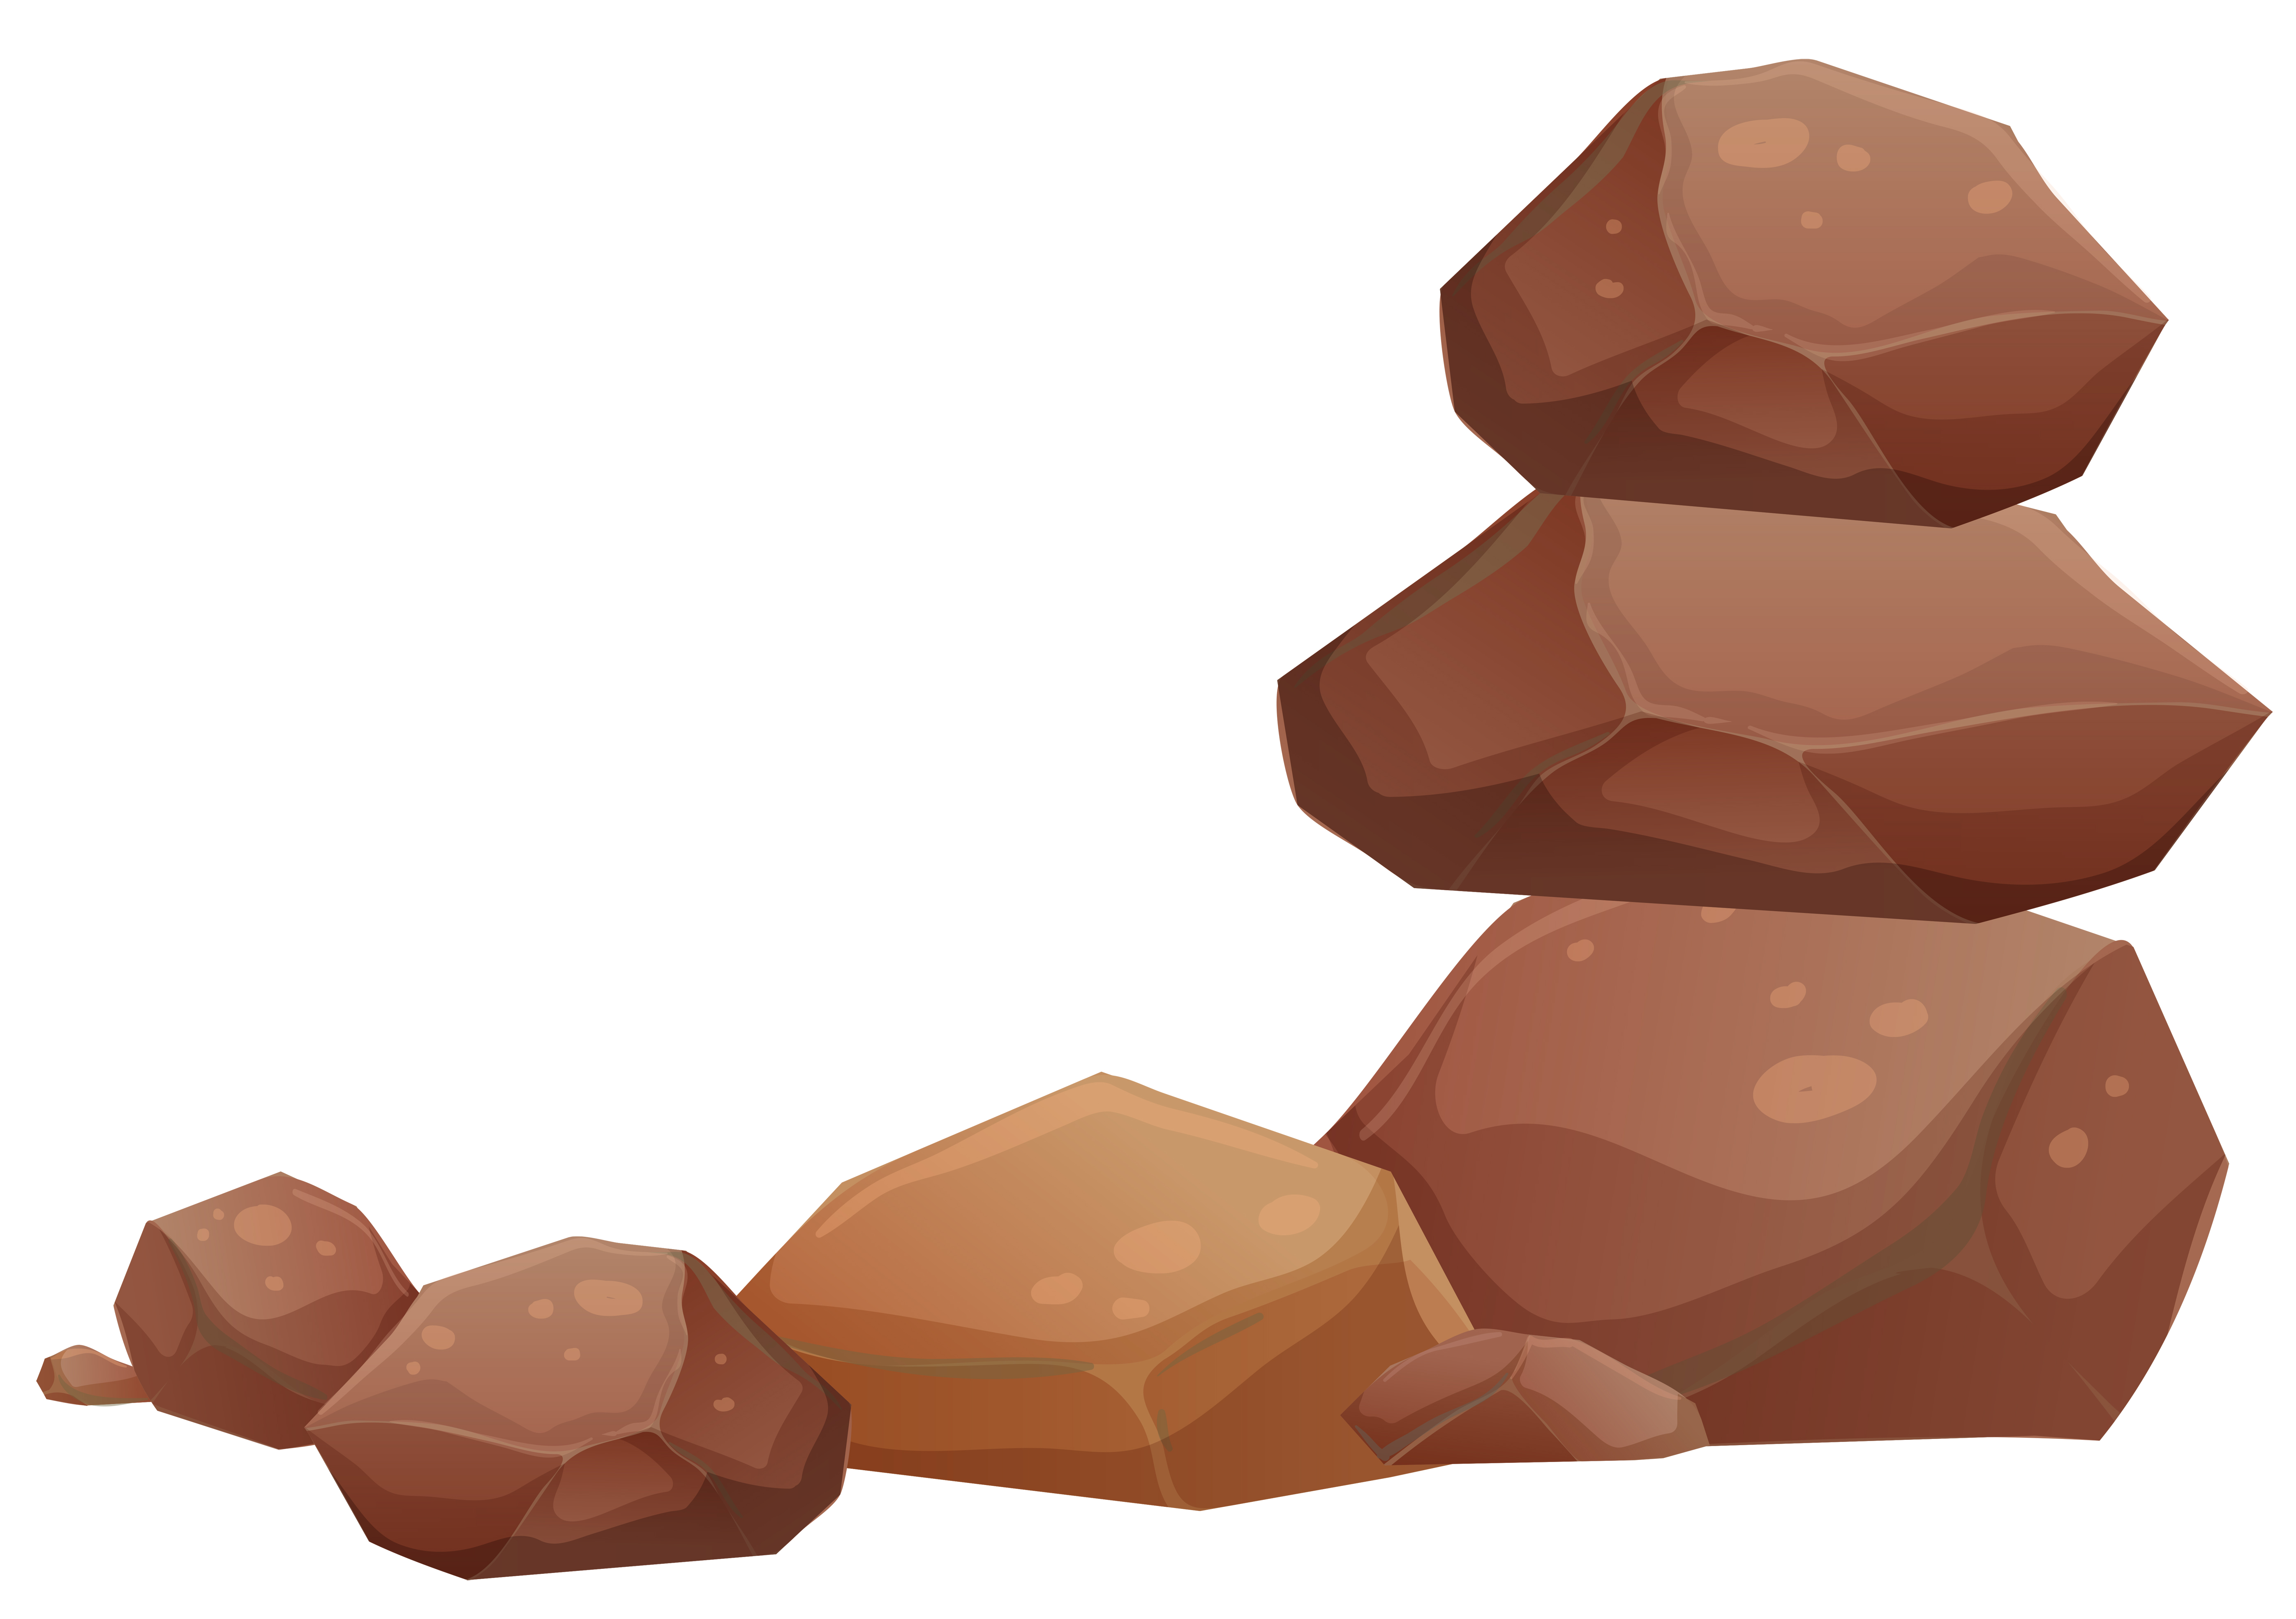
\includegraphics[width=.25\textwidth]{media/image56.jpg}
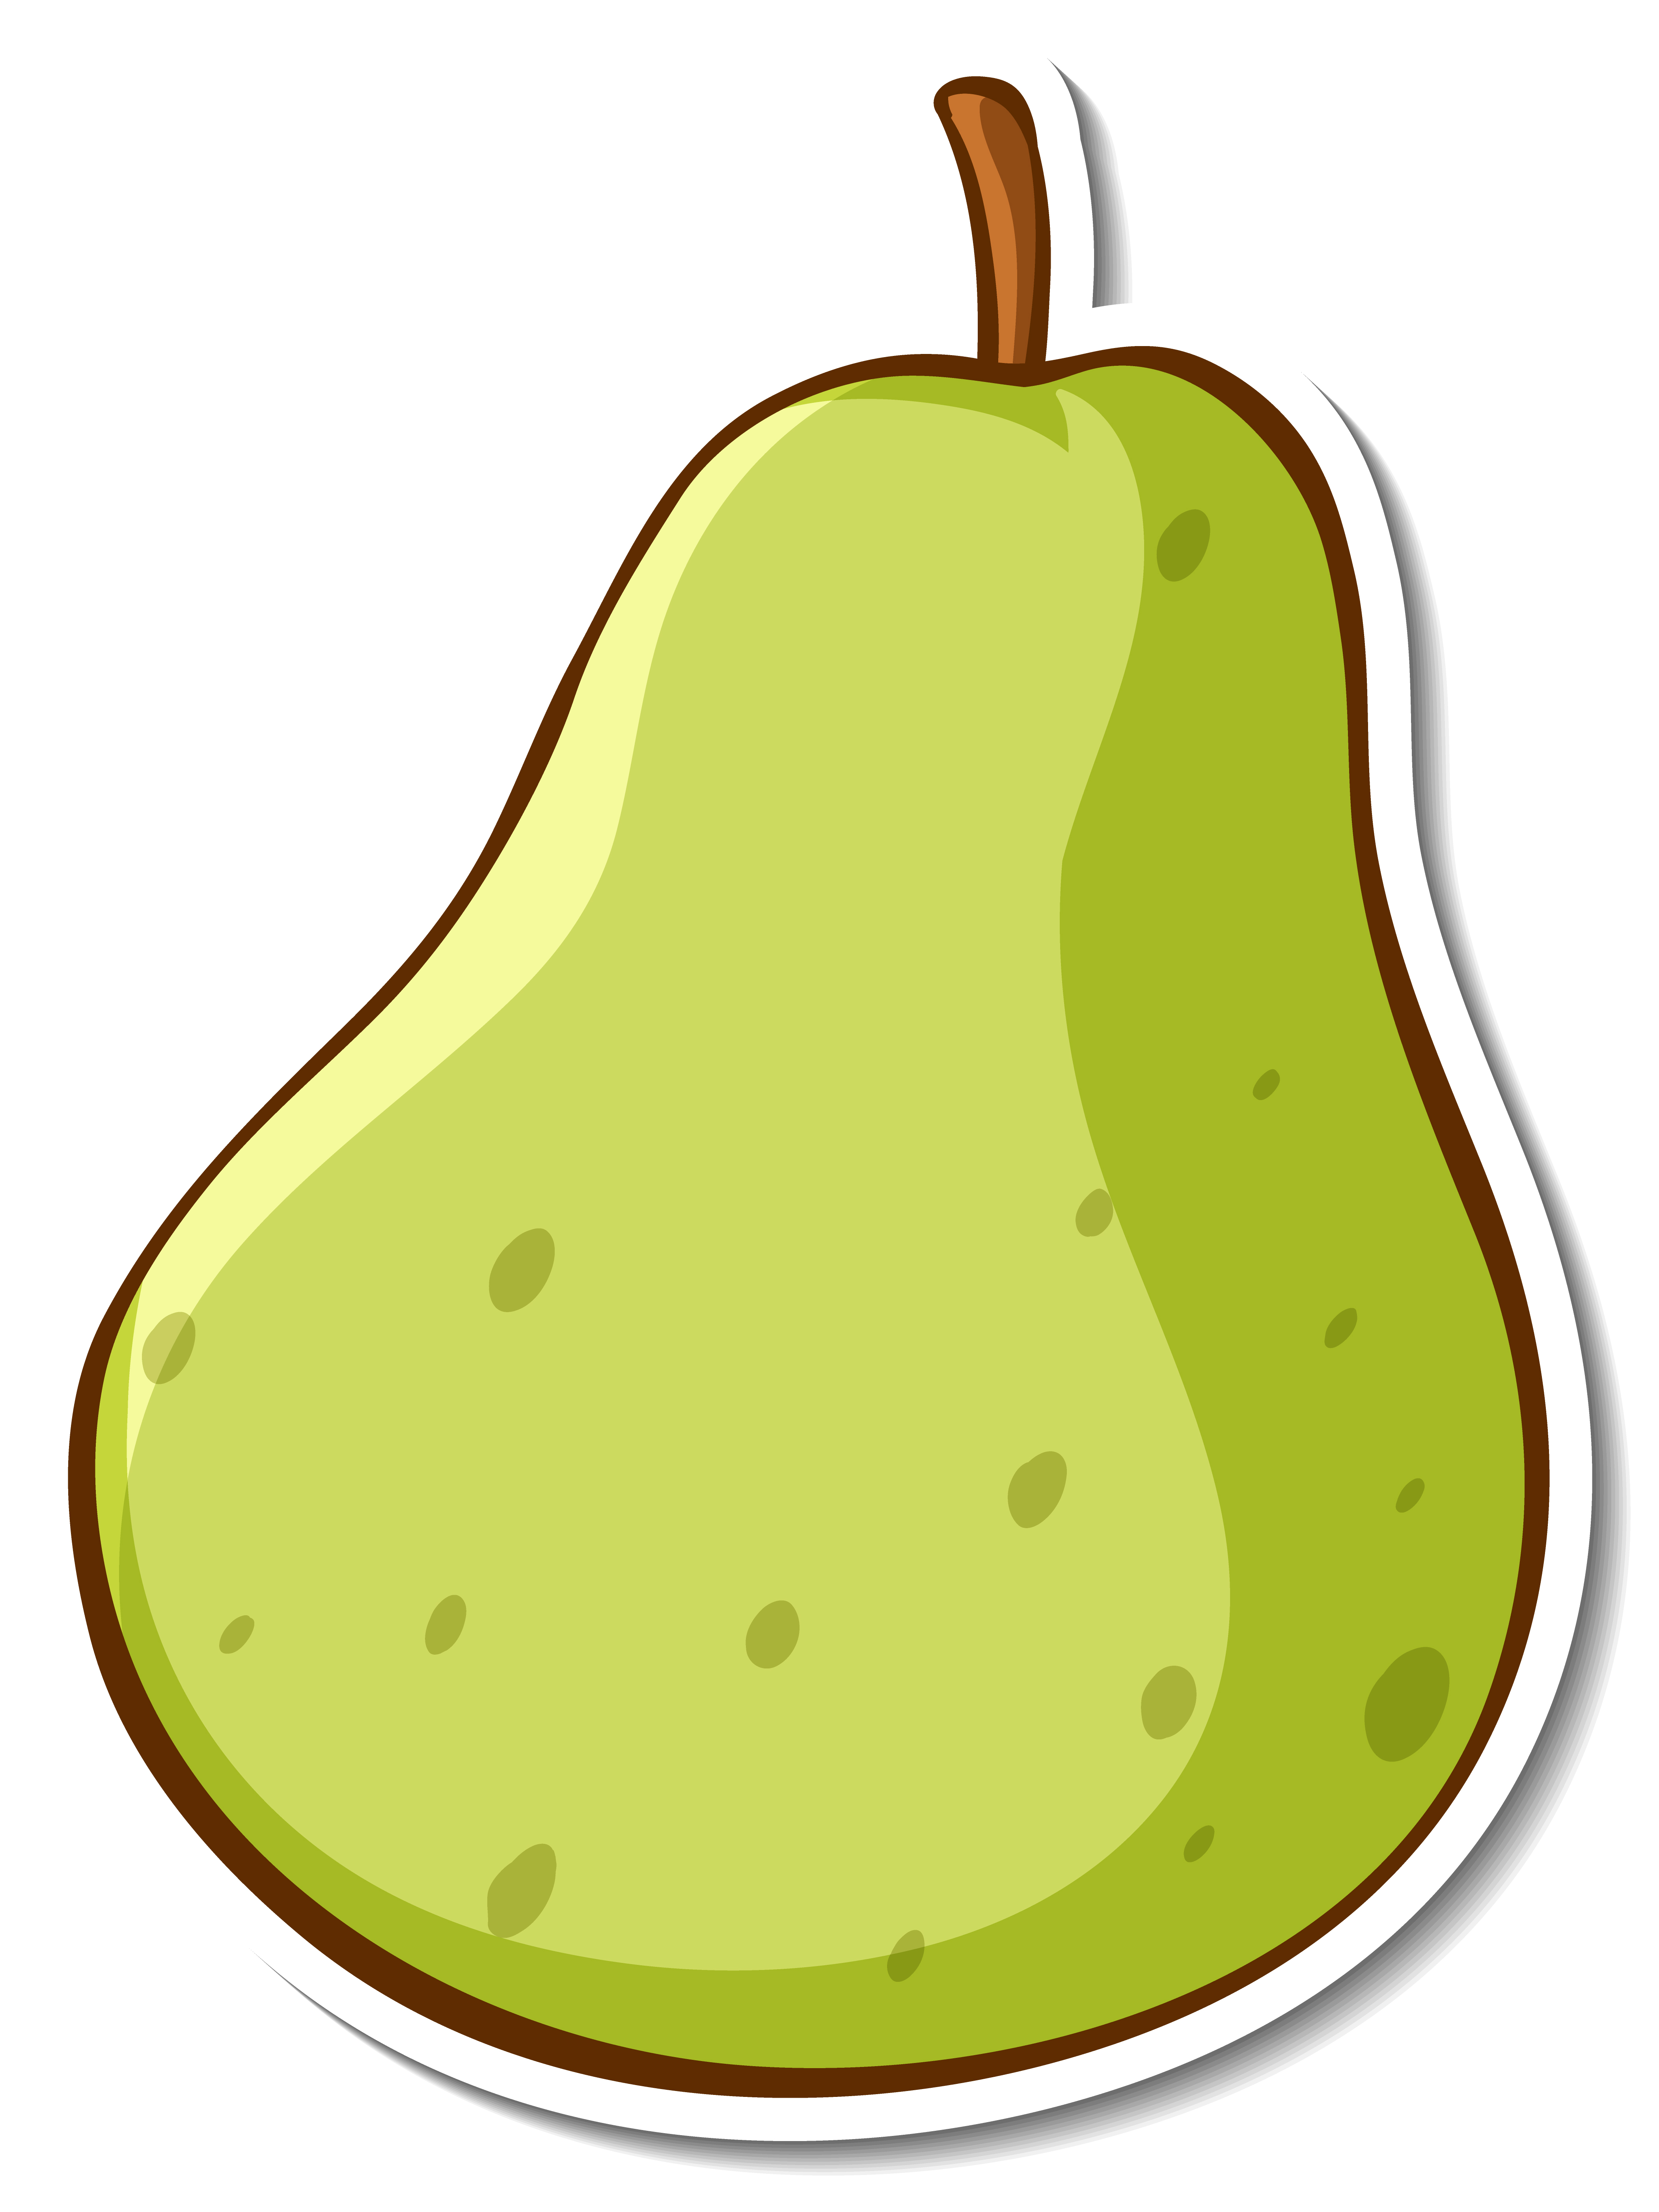
\includegraphics[width=.15\textwidth]{media/image57.jpg}
\end{figure}
\enlargethispage{2\baselineskip}

\reduline{Unha\hfill}

\reduline{Pera\hfill}

\reduline{Pedra\hfill}

\num{3} Ligue as palavras aos seus respectivos desenhos.

%\coment{Leve para sala as palavras dentro de uma sacola. Cada criança deve pegar uma palavra da sacola para fazer a leitura. Depois proponha a atividade.}

\begin{table}[H]
\centering
\begin{tabular}{cp{7cm}c}
Bicicleta & & 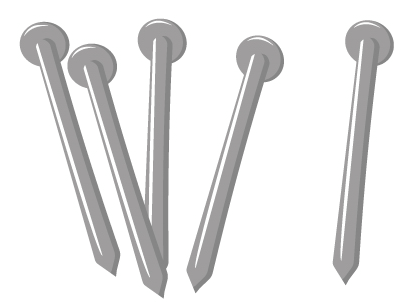
\includegraphics[width=.3\textwidth]{media/image59.png} \\
Borboleta & & 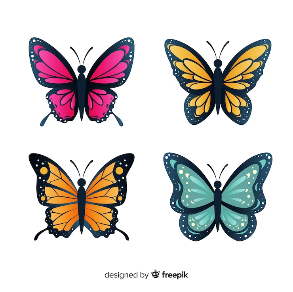
\includegraphics[width=.3\textwidth]{media/image61.png} \\
Dragão & & 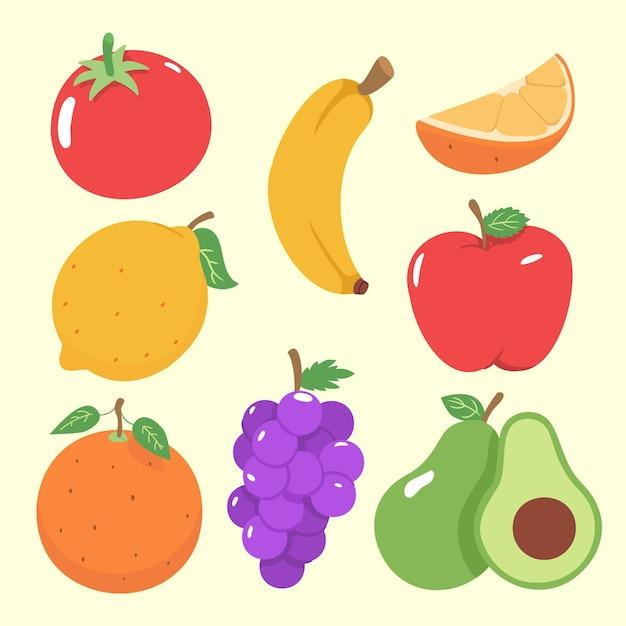
\includegraphics[width=.4\textwidth]{media/image62.jpg} \\
Avião & & 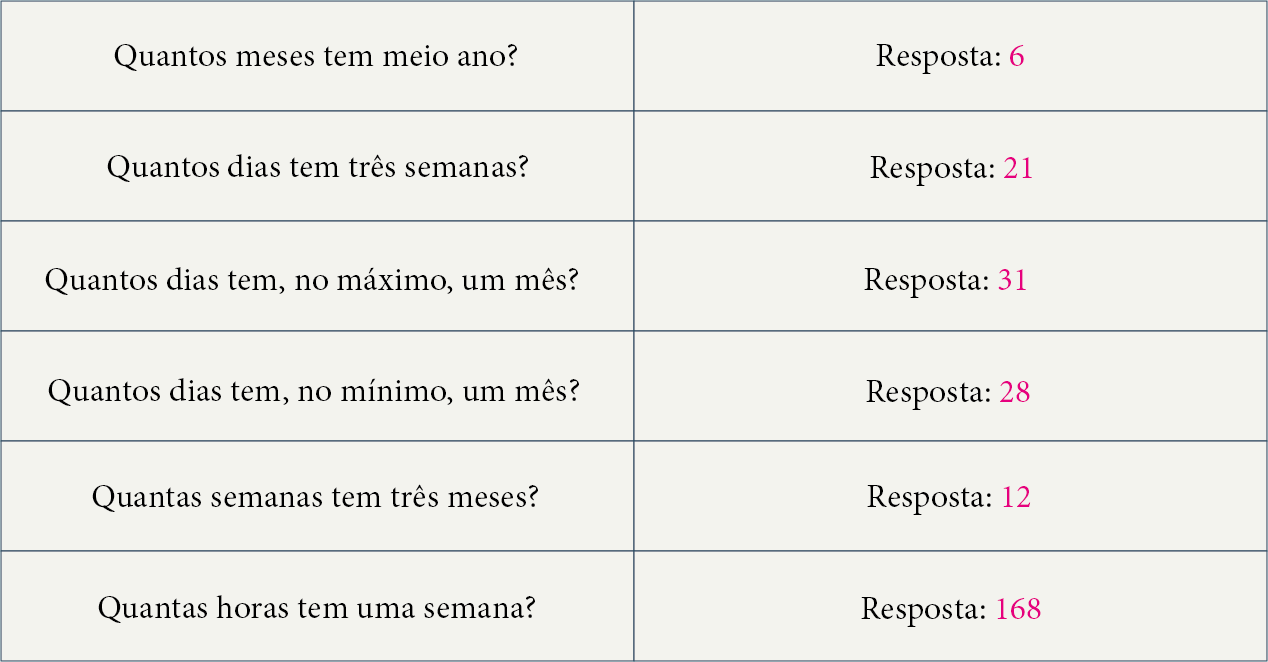
\includegraphics[width=.4\textwidth]{media/image50.png} \\
Prego & & 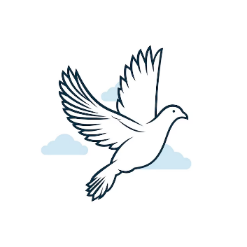
\includegraphics[width=.23\textwidth]{media/image66.png} \\
Pomba & & 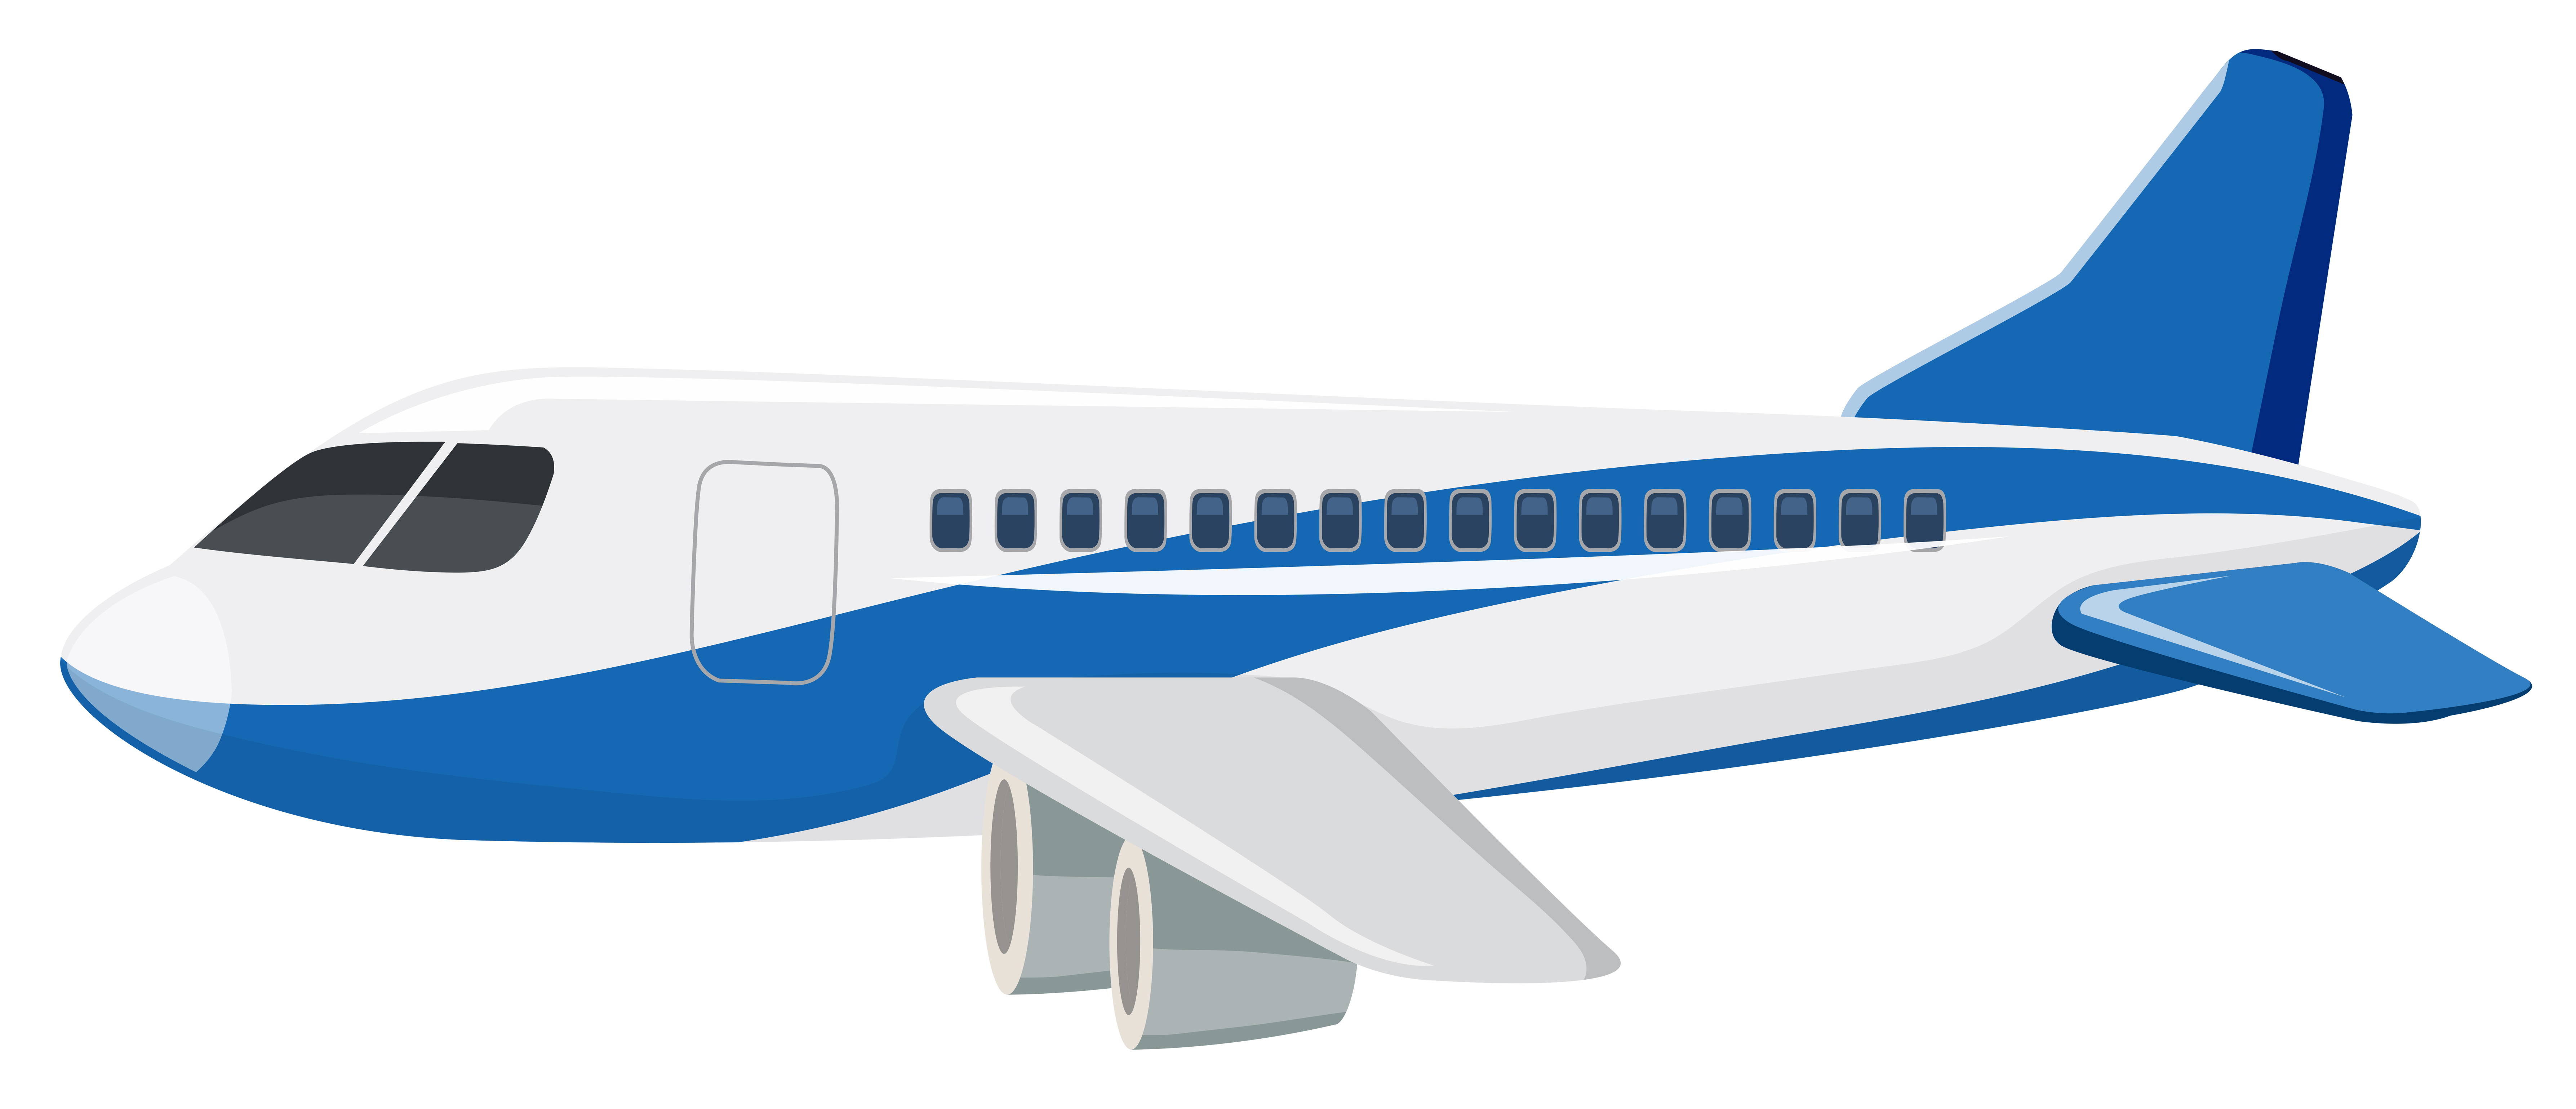
\includegraphics[width=.4\textwidth]{media/image65.jpg}
\end{tabular}
\end{table}

\num{4} Pinte no diagrama as palavras do quadro abaixo.

\vspace*{+2em}

%\coment{Faça a leitura das palavras com os alunos aproveite esse momento para trabalhar a função da escrita.}

\begin{quote}\parindent=0em
\vspace*{-.5cm}
\begin{multicols}{3}
PIÃO

CAMA

LEÃO

PEDRA

ABACATE

SAPO

PATO

SABÃO

TRATOR

GRAMA

CISNE
\end{multicols}
\end{quote}

\begin{longtable}[]{@{}llllllllll@{}}
\toprule
P & I & Ã & O & D & O & W & E & I & S\tabularnewline
F & H & P & I & S & A & B & Ã & O & A\tabularnewline
S & J & L & S & J & U & Y & U & J & P\tabularnewline
L & O & A & B & A & C & A & T & E & O\tabularnewline
E & U & I & D & A & S & A & L & K & A\tabularnewline
à & A & B & G & C & A & Y & J & G & P\tabularnewline
O & S & A & P & A & T & O & P & R & E\tabularnewline
Z & D & R & F & D & M & E & C & A & D\tabularnewline
L & T & R & A & T & O & R & Q & M & R\tabularnewline
B & U & G & T & E & Y & E & C & A & A\tabularnewline
A & C & I & S & N & E & O & P & U & O\tabularnewline
L & O & L & O & C & A & M & A & A & G\tabularnewline
\bottomrule
\end{longtable}

%\coment{R: pião -- cama -- leão- pedra- abacate- sapo- cama- pato -- sabão -- trator -- grama- cisne.}

\num{5} Coloque o til nas palavras sempre que necessário.

\vspace*{+1em}

%\coment{Construa com os alunos critérios para identificar as marcas de nasalidade de uma palavra. Sugira que leiam as palavras em voz alta e posicionem os dedos indicador e polegar sobre o nariz ao pronunciar palavras com esses sons, para perceberem a diferença, por exemplo, entre a pronúncia de palavras como \textit{lá} e \textit{lã}, \textit{manha} e \textit{manhã}. Explique que o til acompanha apenas as vogais A e O.}

\begin{multicols}{3}
IRMAO

SALA

MAO

PATO

MAÇA

VILA

MOLA

MANHA

LA
\end{multicols}

\num{6} Observe a marca de nasalização e complete as palavras com M ou N.

\vspace*{+1em}

%\coment{Siga as orientações da questão anterior, aguçando a atenção das crianças quanto à diferença de pronúncia de palavras como \textit{pote} e \textit{ponte} e \textit{rapa} e \textit{rampa}. Reforce a ideia de M sempre antes de B, e N antes de outras consoantes.}

\begin{multicols}{3}
LÂ\reduline{M}PADA

CA\reduline{M}PO

LARA\reduline{N}JA

TRO\reduline{N}CO

VE\reduline{N}TO

PO\reduline{M}BA

U\reduline{M}BIGO

PO\reduline{N}TE

RA\reduline{M}PA

BO\reduline{M}BOM

TE\reduline{M}PO

PI\reduline{N}TA
\end{multicols}

\pagebreak
\num{7} Leia as frases a seguir e faça um desenho para representar.

%\coment{Oriente a leitura das frases explorando com as crianças o conteúdo de cada uma delas e as diferentes possibilidades de representação.}

\begin{myquote}
\centering
O CAVALO GOSTA DE CORRER.
\end{myquote}

\begin{mdframed}[linewidth=2pt,linecolor=salmao]
\vspace{7,5cm}
\end{mdframed}

\begin{myquote}
\centering
O MENINO JOGA BOLA.
\end{myquote}

\begin{mdframed}[linewidth=2pt,linecolor=salmao]
\vspace{7,5cm}
\end{mdframed}

\begin{myquote}
\centering
O PÁSSARO CANTA FELIZ.
\end{myquote}

\begin{mdframed}[linewidth=2pt,linecolor=salmao]
\vspace{7,5cm}
\end{mdframed}

\begin{myquote}
\centering
A ÁRVORE CAIU.
\end{myquote}

\begin{mdframed}[linewidth=2pt,linecolor=salmao]
\vspace{7,5cm}
\end{mdframed}

%\coment{Respostas pessoais dos alunos.}

\pagebreak

\num{8} Observe as imagens e escreva uma frase para cada uma.
\enlargethispage{\baselineskip}

%\coment{Explore as imagens com as crianças e oriente a construção das frases.}

\begin{figure}[H]
\centering
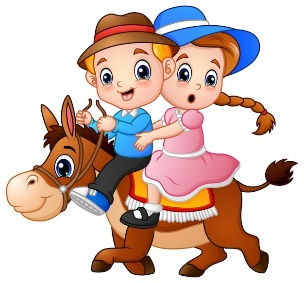
\includegraphics[width=.55\textwidth]{media/image67.jpeg}
\end{figure}

\reduline{Uma resposta possível é \textit{As crianças andam a cavalo}.\hfill}
\linhas{1}

\begin{figure}[H]
\centering
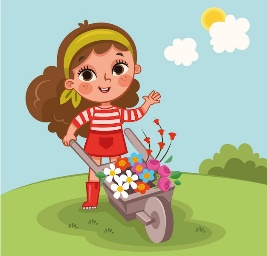
\includegraphics[width=.6\textwidth]{media/image68.jpeg}
\end{figure}

\reduline{Uma resposta possível é \textit{A menina leva flores no carrinho}.\hfill}
\linhas{1}

\num{9} Forme palavras a partir da soma dos números da sílabas.

%\coment{Oriente os alunos a formar as palavras. Em seguida, trabalhe a função social de cada palavra para facilitar a construção das frases.}

\begin{longtable}[]{@{}lllll@{}}
\toprule
\begin{minipage}[b]{0.19\columnwidth}\raggedright\strut
1

BO\strut
\end{minipage} & \begin{minipage}[b]{0.19\columnwidth}\raggedright\strut
2

PI\strut
\end{minipage} & \begin{minipage}[b]{0.19\columnwidth}\raggedright\strut
3

NE\strut
\end{minipage} & \begin{minipage}[b]{0.19\columnwidth}\raggedright\strut
4

CO\strut
\end{minipage} & \begin{minipage}[b]{0.19\columnwidth}\raggedright\strut
5

ÃO\strut
\end{minipage}\tabularnewline
\midrule
\endhead
\begin{minipage}[t]{0.19\columnwidth}\raggedright\strut
6

CAM\strut
\end{minipage} & \begin{minipage}[t]{0.19\columnwidth}\raggedright\strut
7

BRA\strut
\end{minipage} & \begin{minipage}[t]{0.19\columnwidth}\raggedright\strut
8

CIS\strut
\end{minipage} & \begin{minipage}[t]{0.19\columnwidth}\raggedright\strut
9

CA\strut
\end{minipage} & \begin{minipage}[t]{0.19\columnwidth}\raggedright\strut
10

ÇO\strut
\end{minipage}\tabularnewline
\midrule
\begin{minipage}[t]{0.19\columnwidth}\raggedright\strut
11

MA\strut
\end{minipage} & \begin{minipage}[t]{0.19\columnwidth}\raggedright\strut
12

JA\strut
\end{minipage} & \begin{minipage}[t]{0.19\columnwidth}\raggedright\strut
13

LA\strut
\end{minipage} & \begin{minipage}[t]{0.19\columnwidth}\raggedright\strut
14

CA\strut
\end{minipage} & \begin{minipage}[t]{0.19\columnwidth}\raggedright\strut
15

PO\strut
\end{minipage}\tabularnewline
\bottomrule
\end{longtable}

\begin{itemize}
\item 1 + 3 + 14 \reduline{boneca\mbox{ }\hfill}

\item 7 + 10 \reduline{\mbox{ }\hfill}

\item 2 + 5 \reduline{\mbox{ }\hfill}

\item 6 + 15 \reduline{\mbox{ }\hfill}

\item 8 + 3 \reduline{\mbox{ }\hfill}

\item 12 + 3 + 13 \reduline{\mbox{ }\hfill}

\item 11 + 9 + 4 \reduline{\mbox{ }\hfill}
\end{itemize}

\vspace*{+1em}

\num{10} Complete os nomes das frutas com as vogais corretas.

%\coment{Reapresente as vogais aos alunos de acordo com as palavras do exercício. Forme as palavras ressaltado sempre que não existe sílaba sem vogal.}

\vspace*{+1em}

\begin{figure}[H]
\centering
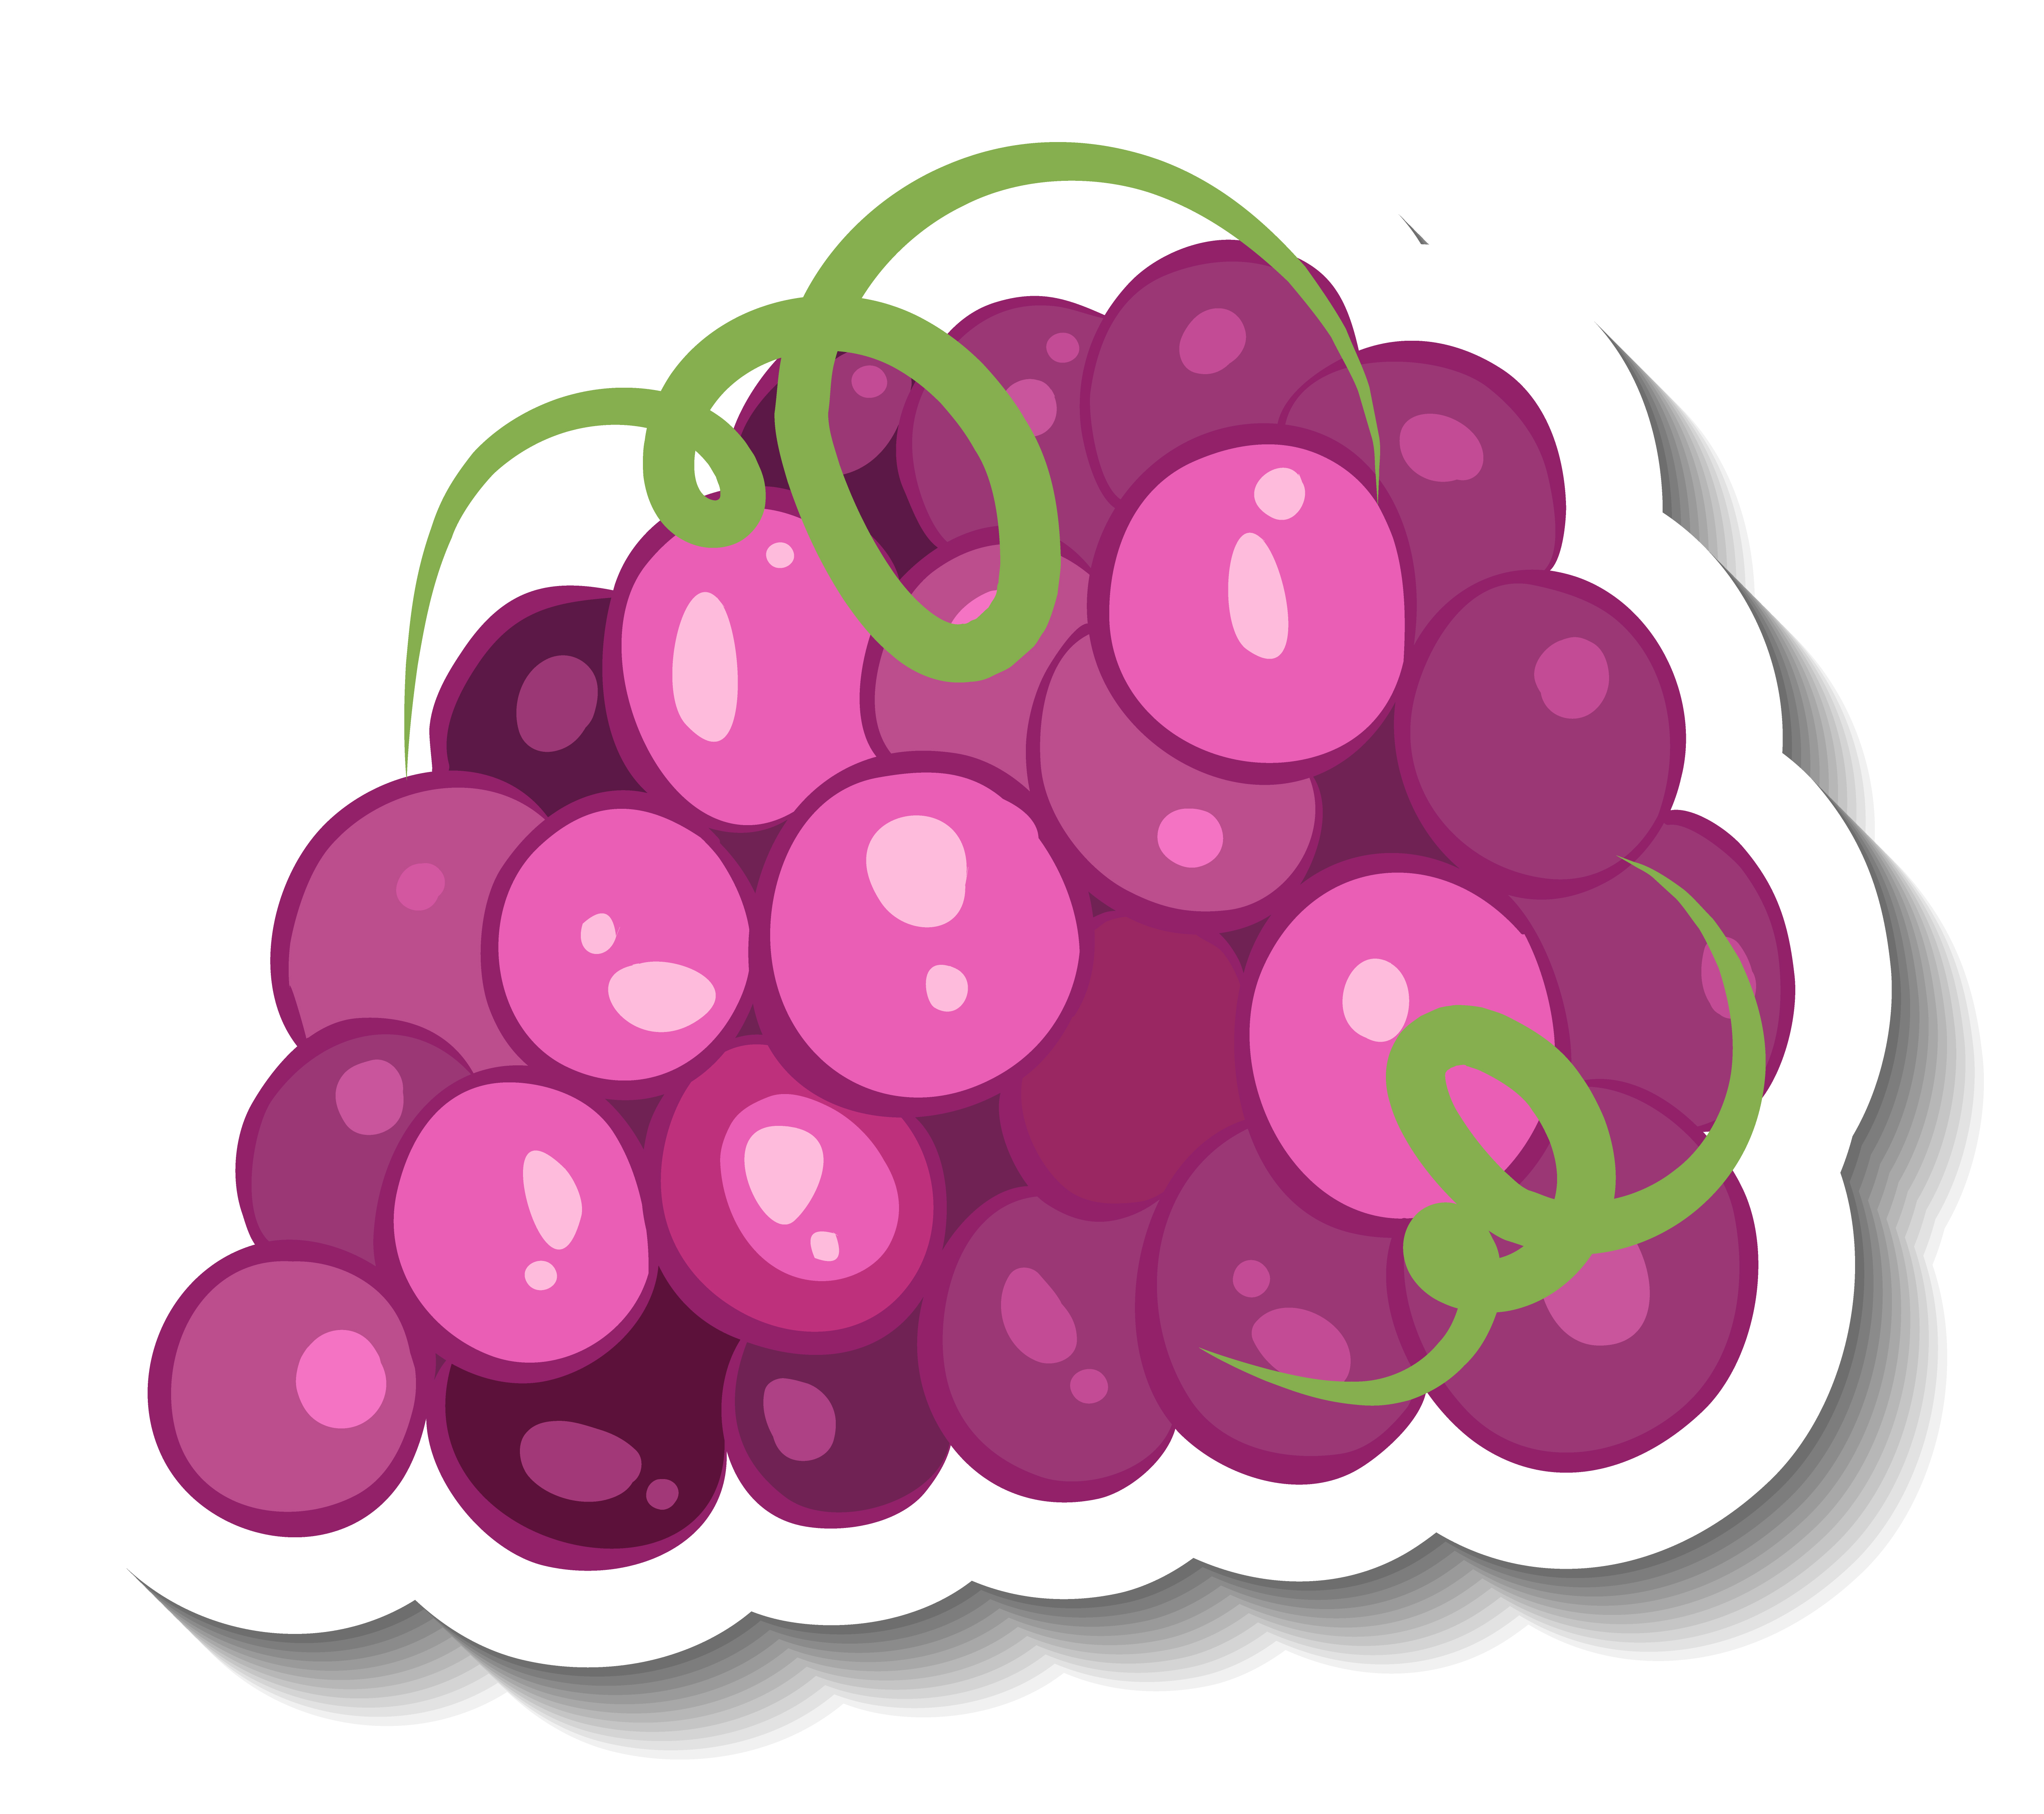
\includegraphics[width=.3\textwidth]{media/image69.jpg}
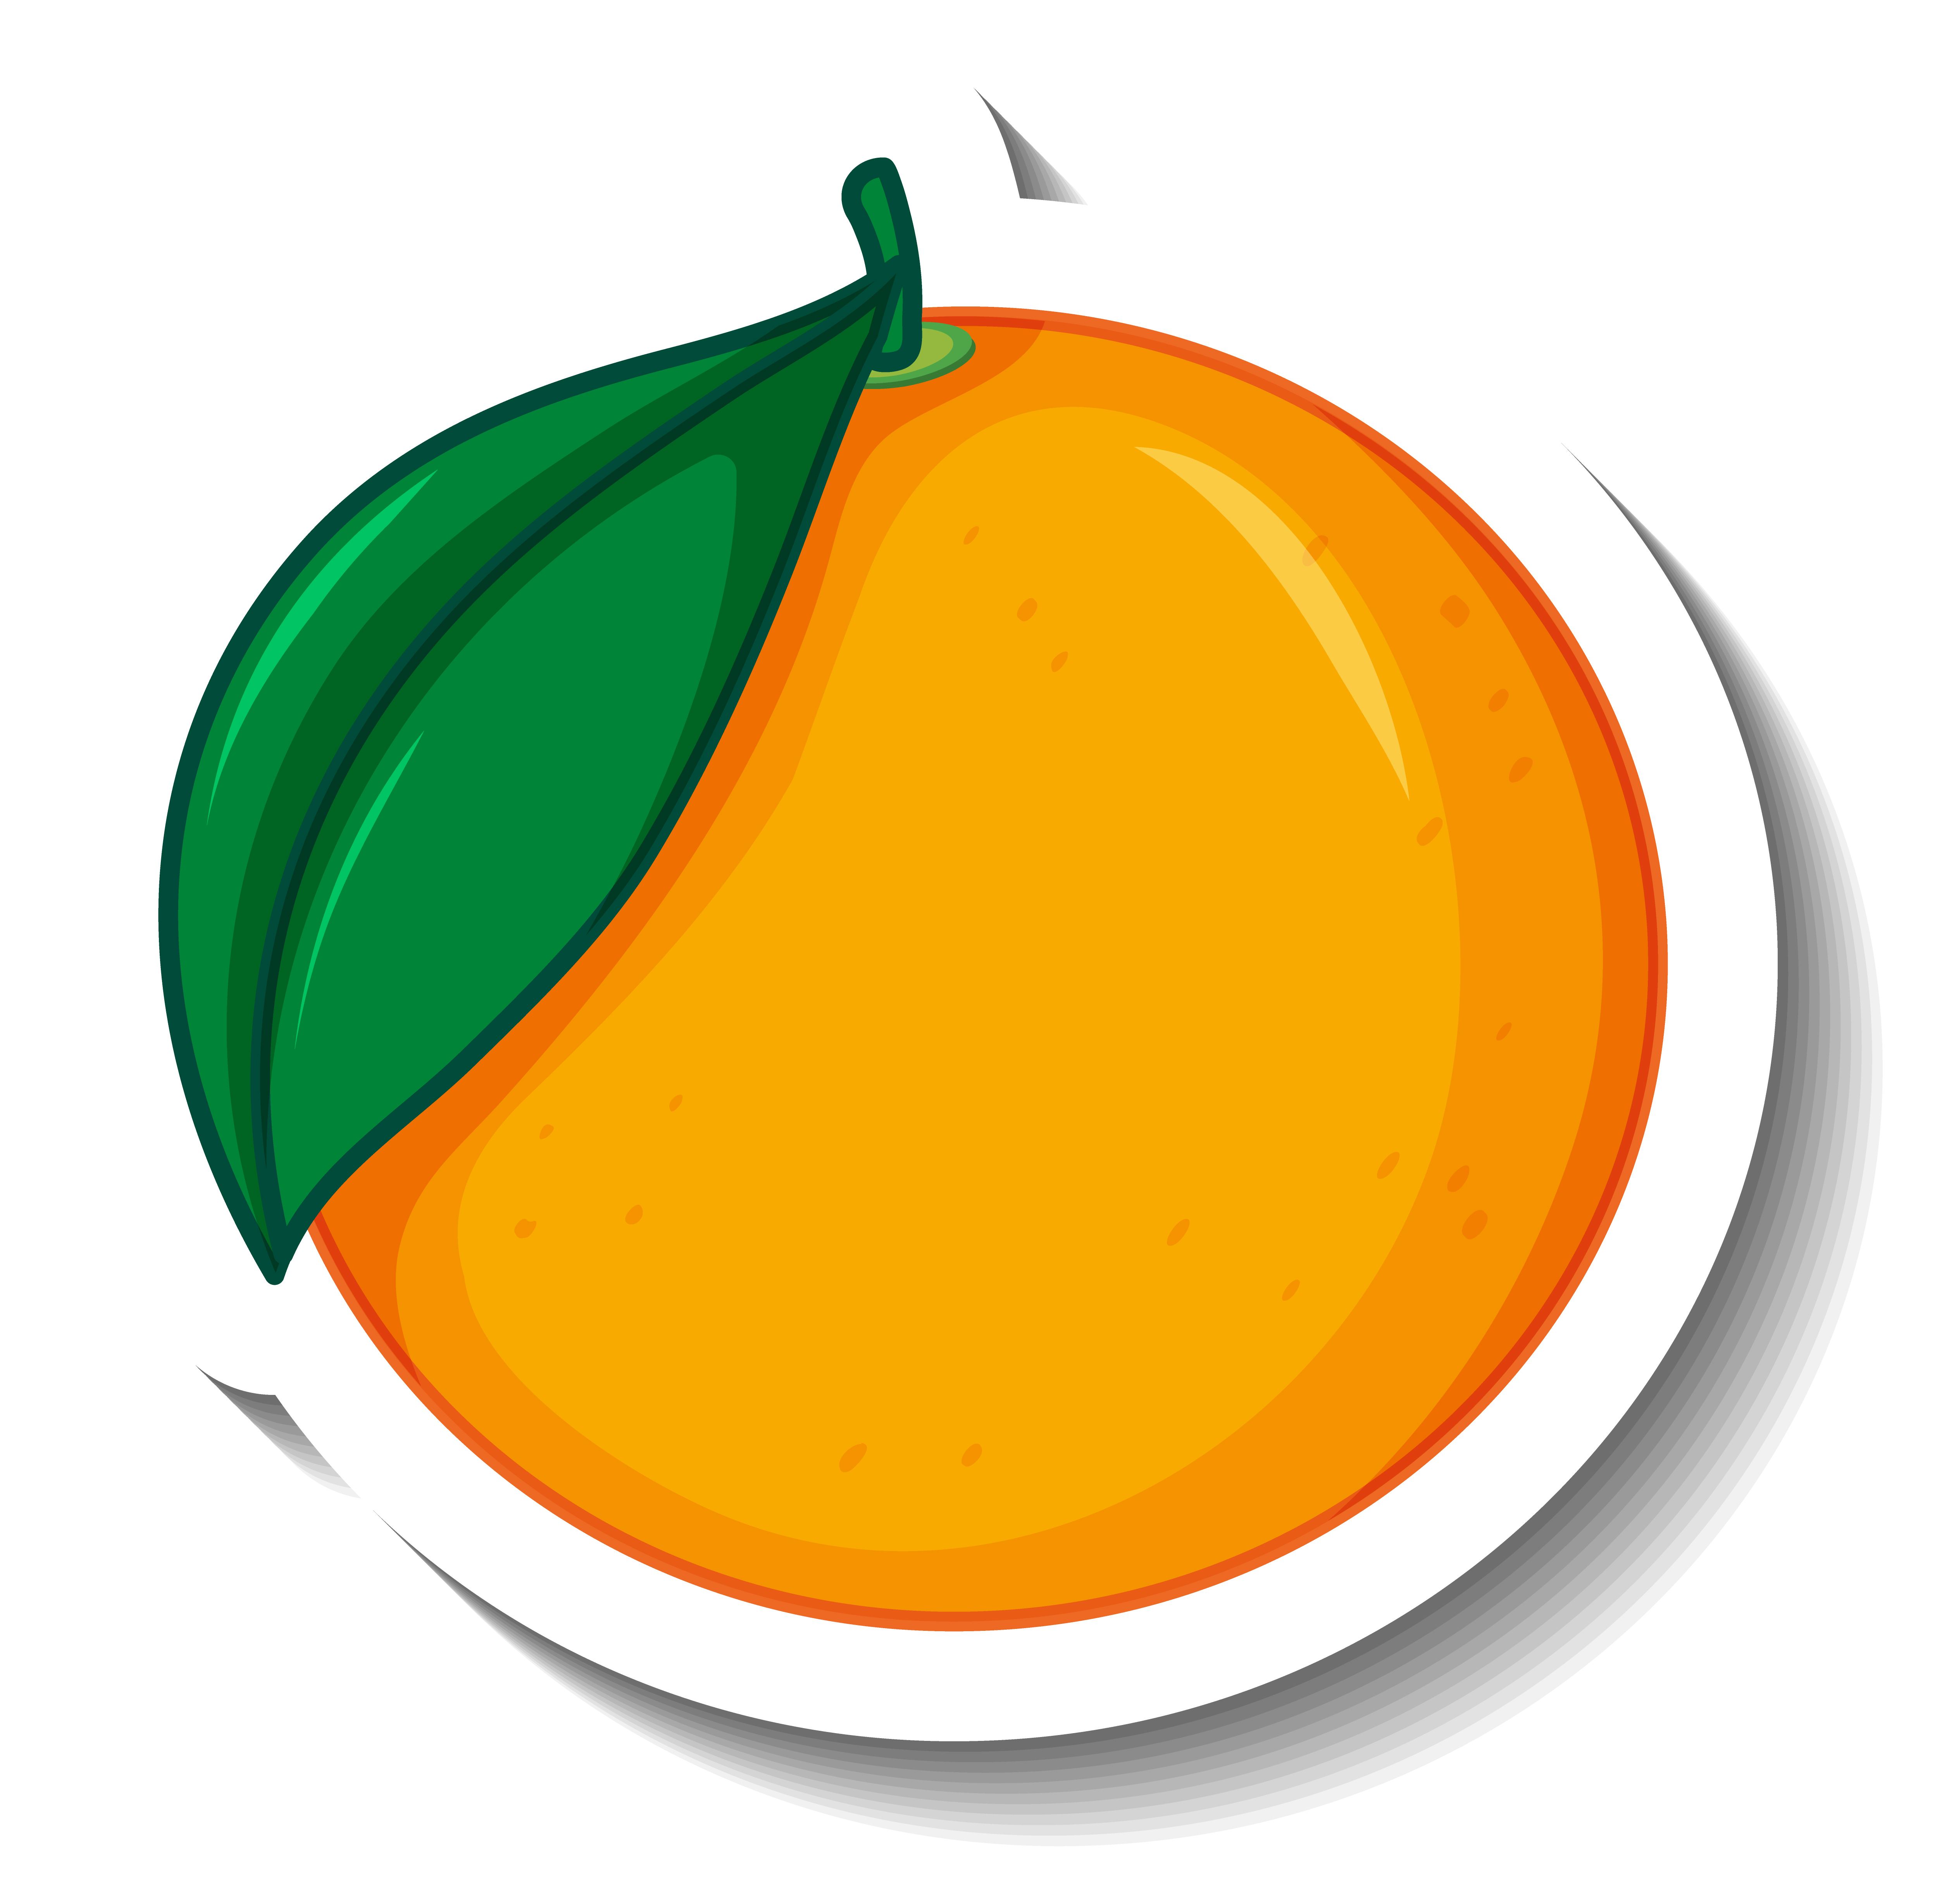
\includegraphics[width=.3\textwidth]{media/image70.jpg}
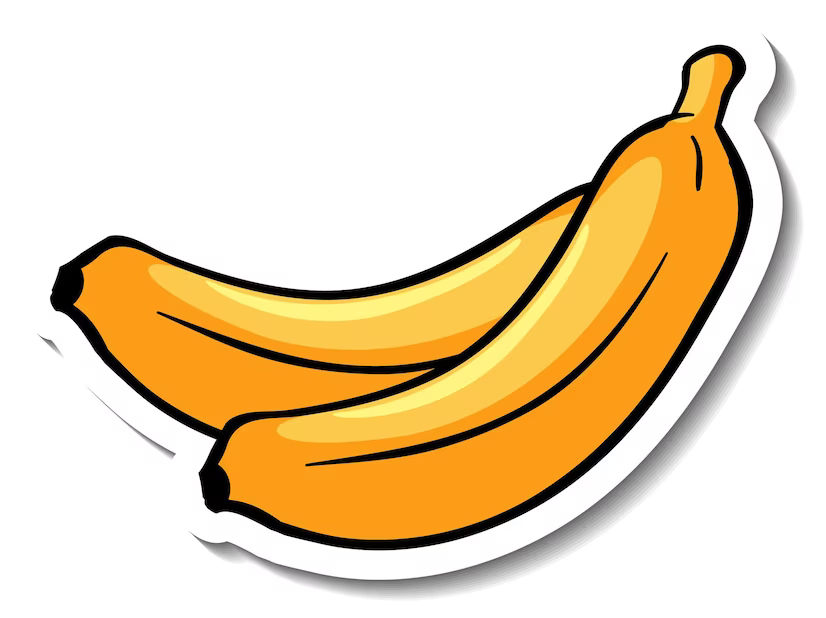
\includegraphics[width=.3\textwidth]{media/image72.png}
\end{figure}

\begin{center}
\reduline{U}V\reduline{A} \hspace{1,5cm} L\reduline{A}R\reduline{A}NJ\reduline{A} \hspace{0,5cm} 
\hspace{1,0cm} B\reduline{A}N\reduline{A}N\reduline{A}
\end{center}

\begin{figure}[H]
\centering
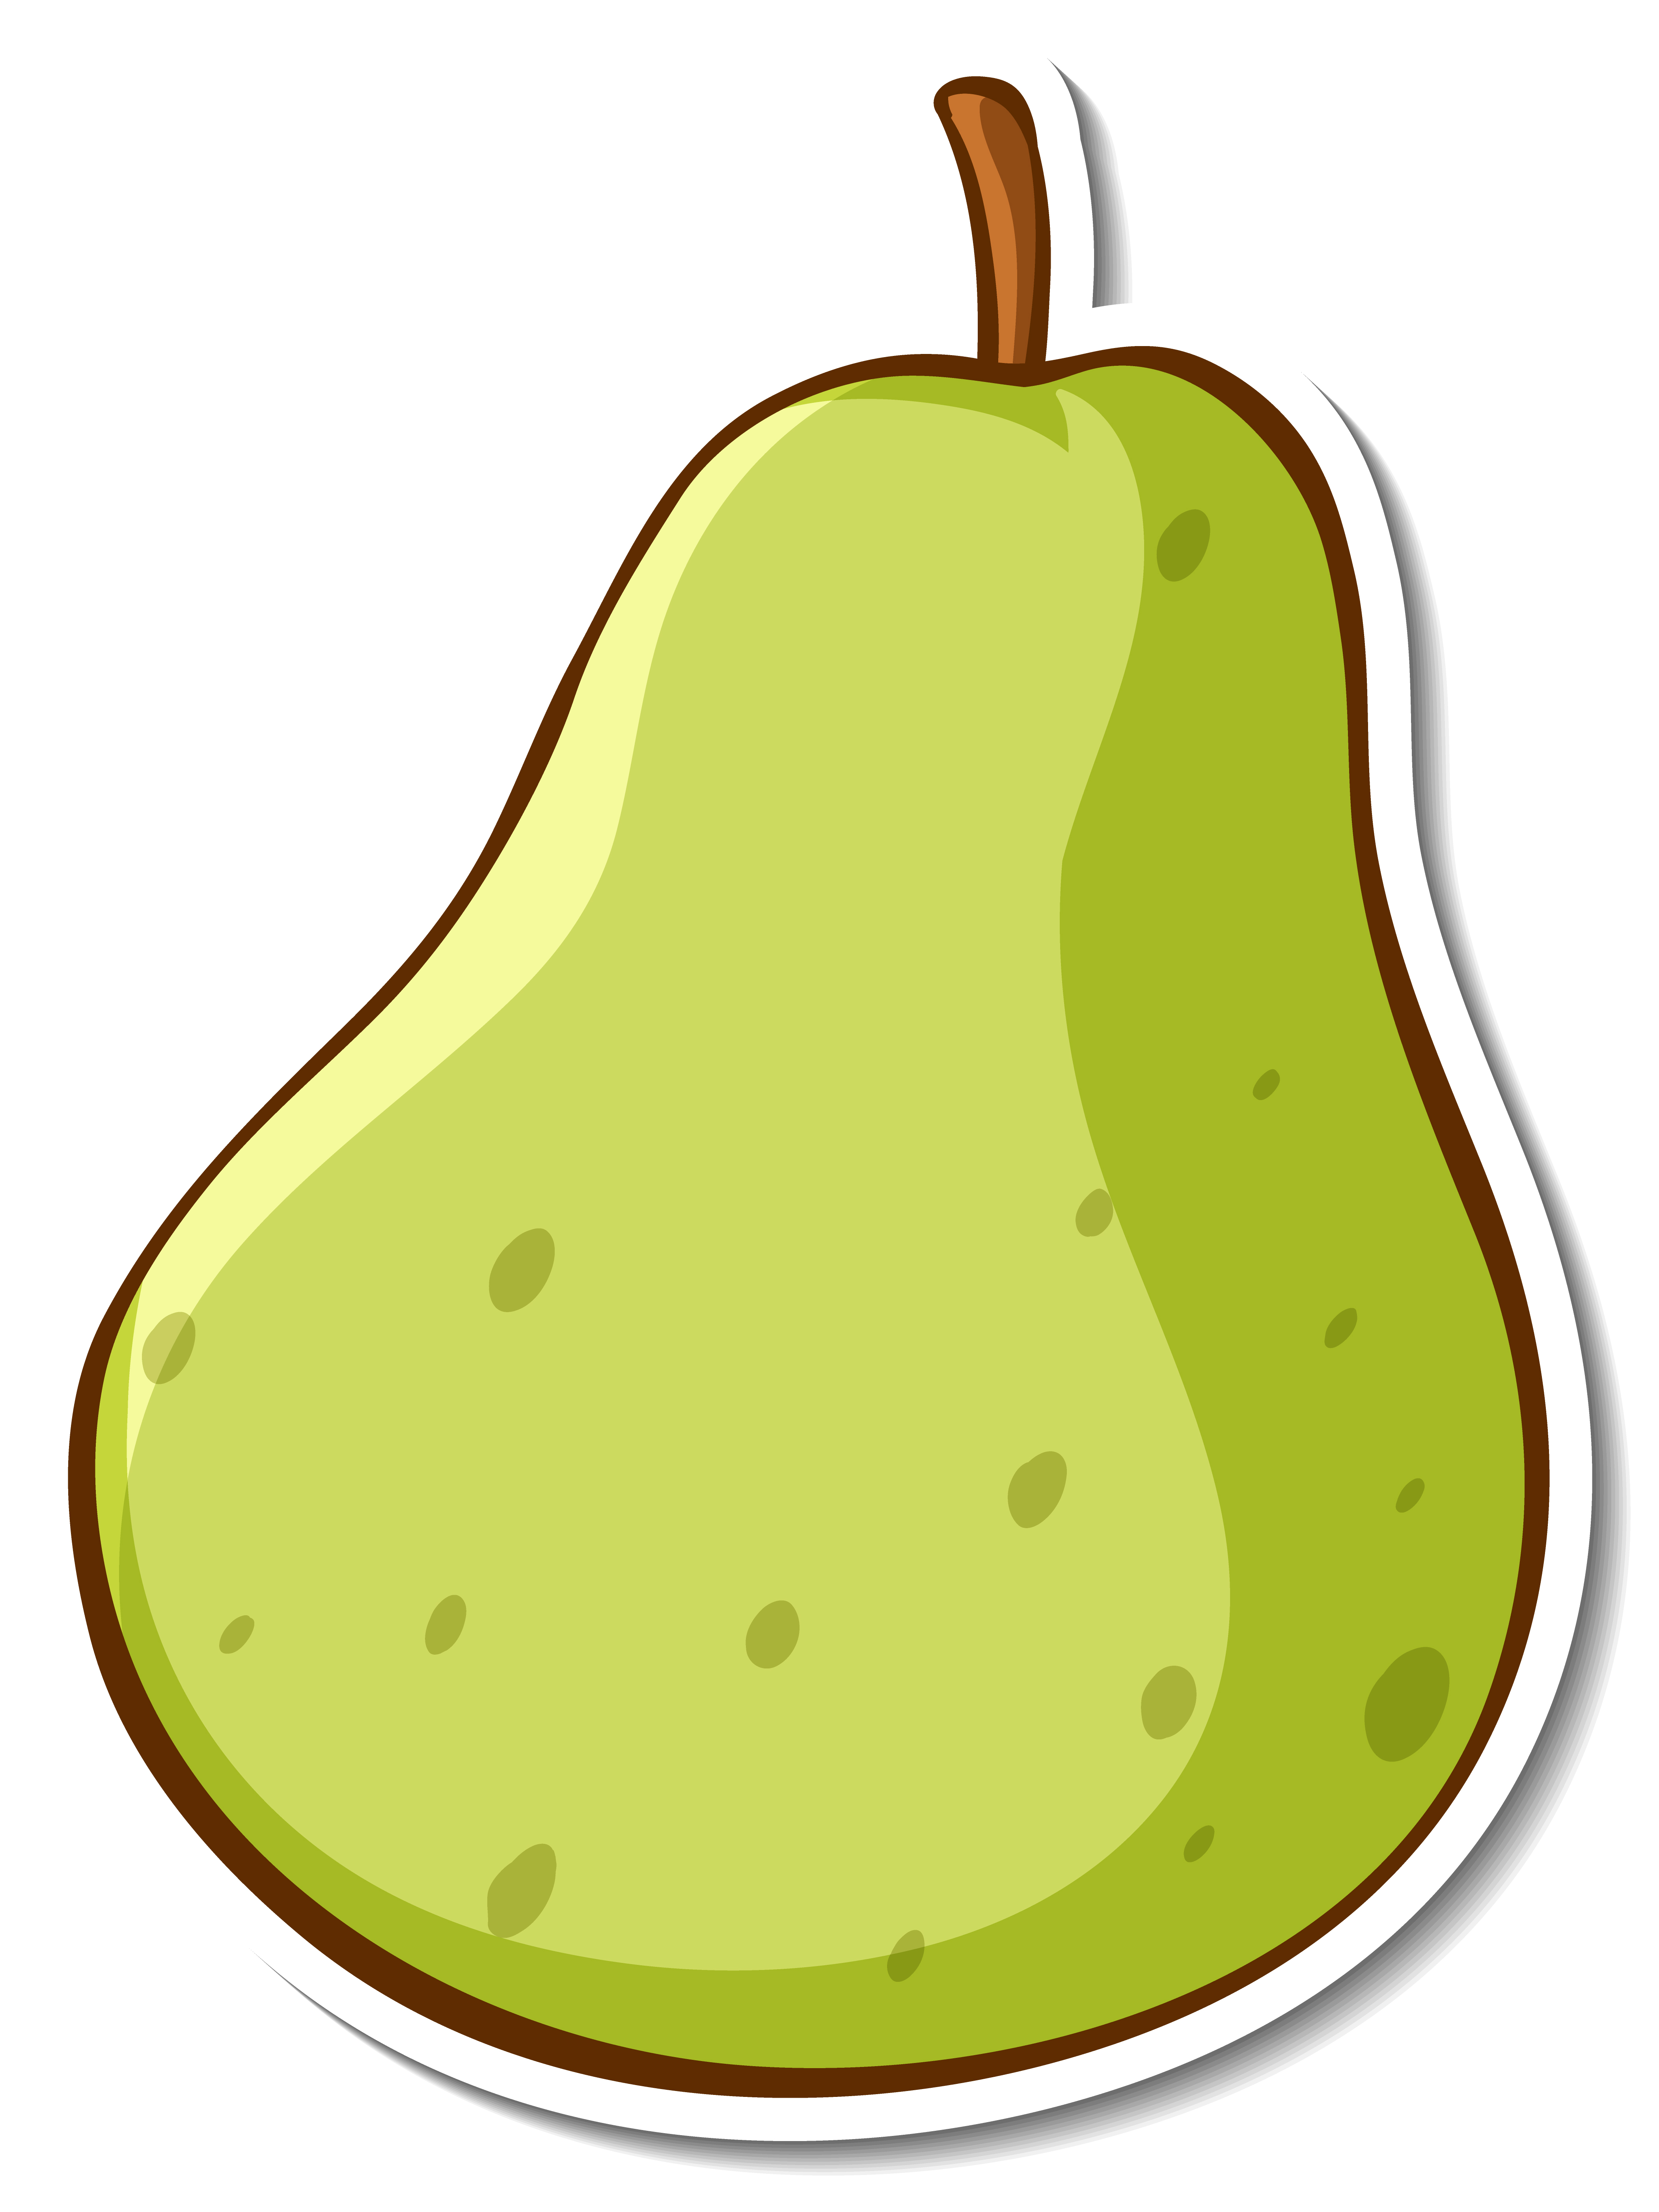
\includegraphics[width=.24\textwidth]{media/image57.jpg}
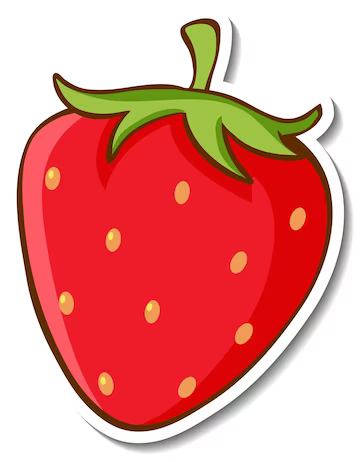
\includegraphics[width=.24\textwidth]{media/image74.png}
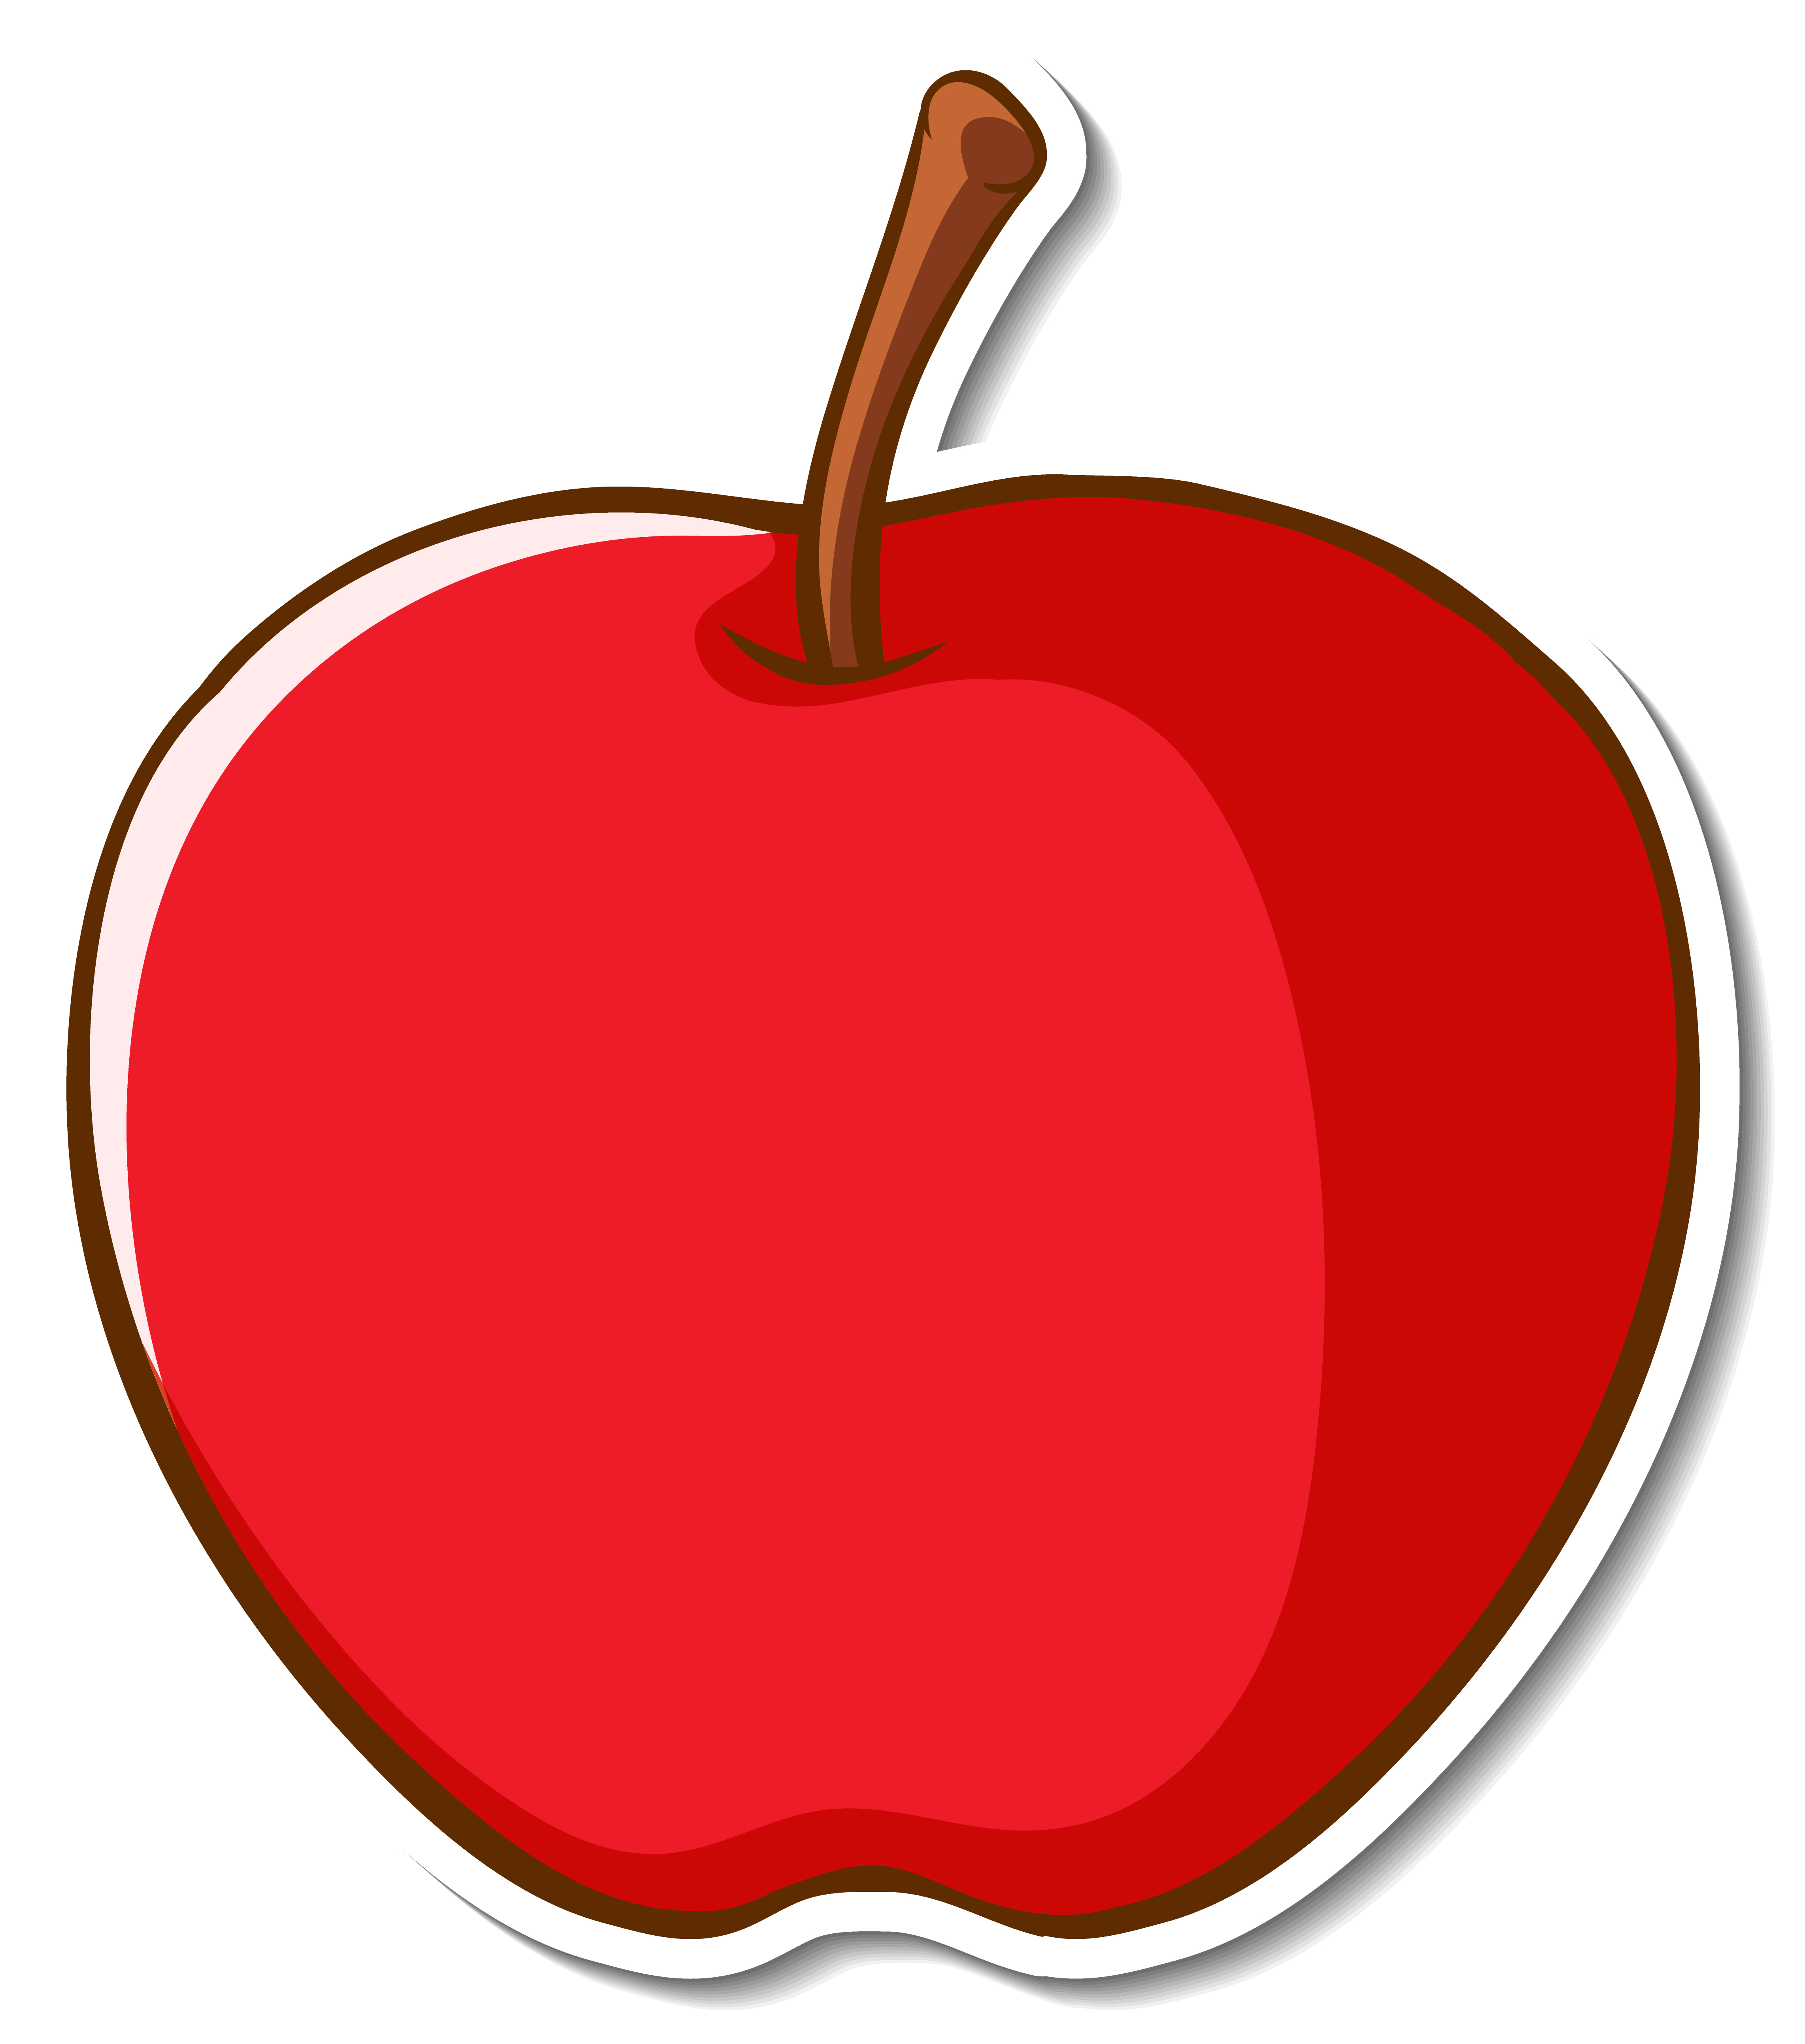
\includegraphics[width=.24\textwidth]{media/image76.jpg}
\end{figure}

\begin{center}
P\reduline{Ê}R\reduline{A} \hspace{1cm} M\reduline{O}R\reduline{A}NG\reduline{O} \hspace{0,5cm} 
\hspace{1cm} M\reduline{A}Ç\reduline{Ã}
\end{center}

% \num{11} Organize as palavras de acordo com sua formação silábica.

% %\coment{Leve o alfabeto para sala. Explore as vogais e as consoantes com os alunos. Realize com eles a formação de algumas palavras, identificado as diferentes formações silábicas. Brincar de \textbf{forca} é uma boa opção para desenvolver essa atividade.}

% \begin{myquote}
% ABACAXI -- TRATOR - GRAVIOLA - PRATO -- CAMPO - CISNE - BAÚ
% \end{myquote}

% {\small
% \begin{tabular}{|l|l|l|l|}
% \hline
% \textbf{\begin{tabular}[c]{@{}l@{}}PALAVRAS COM\\ FORMAÇÃO CV\end{tabular}} & \textbf{\begin{tabular}[c]{@{}l@{}}PALAVRAS COM\\ FORMAÇÃO V\end{tabular}} & \textbf{\begin{tabular}[c]{@{}l@{}}PALAVRAS COM\\ FORMAÇÃO CCV\end{tabular}} & \textbf{\begin{tabular}[c]{@{}l@{}}PALAVRAS COM\\ FORMAÇÃO CVC\end{tabular}} \\ \hline
% \rosa{ABACAXI} & \rosa{GRAVIOLA} & \rosa{TRATOR} & \rosa{CISNE} \\ \hline
% \rosa{GRAVIOLA} & \rosa{ABACAXI} & \rosa{GRAVIOLA} & \rosa{CAMPO} \\ \hline
% \rosa{PRATO} & \rosa{BAÚ} & \rosa{PRATO} &  \\ \hline
% \rosa{CAMPO} &  &  &  \\ \hline
% \rosa{CISNE} &  &  &  \\ \hline
% \rosa{BAÚ} &  &  &  \\ \hline
% \end{tabular}
% }

% \pagebreak
\section*{Treino}

\num{1} Mila ganhou uma boneca de sua tia. A palavra 
cuja primeira sílaba possui a mesma formação da primeira
sílaba do brinquedo de Mila é

% \begin{figure}[htpb!]
% \centering
% 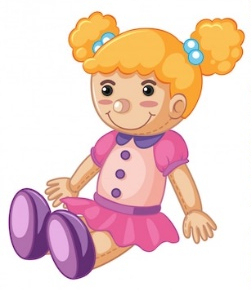
\includegraphics[width=.5\textwidth]{media/image77.jpeg}
% \end{figure}

\begin{escolha}
\item abacate.

\item janela.

\item traça.

\item prego.
\end{escolha}

\vspace*{+1em}

\num{2} Veja a palavra nova que Ana aprendeu a ler.

\vspace*{+1em}

\begin{myquote}
\centering
\textbf{FORMIGA}
\end{myquote}

A primeira sílaba da palavra acima tem a mesma formação que a 
primeira sílaba de

\begin{escolha}
\item borboleta.

\item dragão.

\item laranja.

\item garota.
\end{escolha}

\pagebreak

\num{3} Leia a frase.

\begin{myquote}
\centering
\textbf{A menina brinca com bolhas de sabão.}
\end{myquote}

A imagem que representa o que está escrito na frase é

\begin{escolha}
\item\includegraphics[width=.3\textwidth]{media/image78.png}

\item\includegraphics[width=.3\textwidth]{media/image79.png}

\item\includegraphics[width=.3\textwidth]{media/image80.png}

\item\includegraphics[width=.4\textwidth]{media/image81.png}
\end{escolha}

\chapter[Encontrando informações no texto]{\Large Encontrando informações no texto}
\markboth{Módulo 3}{}

%Para iniciar este módulo, é possível comentar os tipos dos textos que serão lidos e explorar bastante a oralidade, fazendo diversos questionamentos de informações que estão nos textos.

\section*{Habilidade do SAEB}

\begin{itemize}
	\item Localizar informações explícitas em textos
\end{itemize}

\subsection{Habilidades da BNCC}

\begin{itemize}
\item EF15LP03
\end{itemize}

\conteudo{
Leia o poema a seguir.
\begin{verse}
\textbf{Meu galinho}

Há três noites que eu não durmo\\
Ó lá lá\\
Pois perdi o meu galinho\\
O lá lá\\
Coitadinho o lá lá,\\
Pobrezinho o lá lá\\
Se perdeu lá no jardim.

Ele é branco e amarelo\\
O lá lá\\
Tem a crista vermelhinha\\
O lá lá\\
Bate as asas, o lá lá,\\
Abre o bico o lá lá\\
E faz qui qui ri qui qui
\end{verse}

\fonte{Disponível em: http://www.dominiopublico.gov.br/download/texto/me000588.pdf. Acesso em: 19 abr. 2023. }

Por que essa pessoa não dorme?

Onde o galo se perdeu?

Quais são as cores do galo?

Para responder a essas e outras perguntas, você precisa buscar as
informações no texto. Elas estão todas lá, de forma bem clara. 
Basta observar com atenção.

Observe o seguinte cartaz:\bigskip

\begin{center}
\noindent\includegraphics[width=\textwidth]{media/image82.png}\bigskip
\end{center}

Temos um texto chamativo no cartaz dizendo ``Doe um brinquedo, ganhe um sorriso''. A partir dessa frase, já podemos identificar o assunto principal. Além disso, devemos levar em conta também os aspectos visuais da imagem. Ao centro do cartaz, encontramos uma caixa cheia de brinquedos. Colocando essas duas informações juntas, temos certeza, então, do assunto tratado.
}

\section*{Atividades}

\num{1} Vamos cantar.

%\coment{Convide as crianças para brincar com a música, usando o nome dos alunos da turma. Em seguida faça questionamentos sobre a música: onde a canoa virou? Maria estava sozinha? Alguém socorreu Maria?}

\begin{myquote}
\begin{center}
\noindent\includegraphics[width=.6\textwidth]{media/image183.png}\bigskip
\end{center}
\begin{verse}
\textbf{A canoa virou}

A canoa virou,\\
pois deixaram virar.\\
Foi por causa do João,\\
que não soube remar.

Se eu fosse um peixinho\\
e soubesse nadar,\\
eu tirava o João\\
do fundo do mar.
\end{verse}

\fonte{Política Nacional de Alfabetização. Cantigas. Disponível em: https://tinyurl.com/yckw7p6b. Acesso em: 19 abr. 2023.}
\end{myquote}

\begin{escolha}
\item Escreva o título da música.\\
\reduline{A canoa virou.\hfill}
\linhas{1}

\item Por que a canoa virou?\\
\reduline{João não soube remar.\hfill}
\linhas{1}

\item Se eu fosse um peixinho o que eu faria?\\
\reduline{Se eu fosse um peixinho, eu tirava o João do fundo do mar.\hfill}
\linhas{1}
\end{escolha}

\num{2} Vamos brincar de trem?

%\coment{Convide os alunos para formar um trem. Nesse momento, podem ser trabalhadas as noções de \textbf{lateralidade}: frente, trás, entre. Faça os questionamentos orais para trabalhar a fala e a escuta com as crianças.}

\begin{myquote}
\begin{verse}
\textbf{O trem maluco}

O trem maluco,\\
quando sai de Pernambuco,\\
vai fazendo xique-xique\\
até chegar ao Ceará.
\end{verse}
\fonte{Cantiga Popular.}
\end{myquote}

\begin{escolha}
\item De onde o trem sai?\\
\reduline{O trem sai de Pernambuco.\hfill}

\item Para onde o trem vai?\\
\reduline{O trem vai para o Ceará.\hfill}
\end{escolha}

\num{3} Vamos ler a letra da canção.\enlargethispage{2\baselineskip}

\vspace{+1em}

%\coment{Inicialmente, faça a leitura da letra da canção. Em seguida, convide as crianças a cantar. Depois, faça perguntas sobre o conteúdo da letra para trabalhar a oralidade.}

\begin{myquote}
\begin{verse}
\textbf{Borboletinha}

Borboletinha\\
está na cozinha\\
fazendo chocolate\\
para a madrinha\\
poti, poti\\
perna de pau\\
olho de vidro\\
e nariz de pica-pau\\
tchau, tchau
\end{verse}

\fonte{Secretaria de Educação da Prefeitura de Diadema. Borboletinha. Disponível em: https://tinyurl.com/3n5ym7w5. Acesso em: 19 abr. 2023. }
\end{myquote}

\begin{escolha}
\item Encontre e pinte de azul o nome da música.\\
\reduline{O título ``Borboletinha'' deverá ser pintado.\hfill}

\item Onde a borboletinha está?\\
\reduline{A borboletinha está na cozinha.\hfill}

\item O que ela está fazendo?\\
\reduline{A borboletinha está fazendo chocolate.\hfill}

\item Para quem é o chocolate que ela está fazendo?\\
\reduline{A borboletinha está fazendo chocolate para a madrinha.\hfill}
\end{escolha}

\num{4} Observe esse cartaz.

%\coment{Pergunte as crianças o que elas vem no cartaz. Questione se já participaram de alguma campanha ou se já doaram roupas para outras pessoas. Aproveite e fale da importância de ser solidário.}

\begin{figure}[htpb!]
\centering
\includegraphics[width=.6\textwidth]{media/image83.jpeg}
\end{figure}
%\textbf{\url{http://www.saosebastiao.sp.gov.br/noticia.asp?id=N1122020143810.Acesso} 02 mar. 2023}

\enlargethispage{2\baselineskip}
\begin{escolha}
\item Qual é a campanha mostrada no cartaz?\\
\reduline{O cartaz apresenta uma campanha de arrecadação de roupas.\hfill}

\item As roupas devem ser doadas a crianças de que idade?\\
\reduline{As roupas devem ser doadas a crianças de zero a 3 anos.\hfill}
\end{escolha}

\num{5} Vamos ler com atenção a receita a seguir.

%\coment{Leia a receita para as crianças. Depois, pergunte a elas se conhecem esse tipo de texto. Identifique com elas as instruções apresentadas. A seguir, explore o conteúdo da receita, perguntando aos alunos, por exemplo, se conhecem os ingredientes e gostam deles.}

%Paulo: acredito que seria interessante colocar a receita abaixo em um box que lembrasse uma folha de papel, pautada ou não, se possível com uma fonte que lembre letra cursiva. 
\begin{myquote}
\begin{center}
\textbf{Macarrão de panela de pressão}
\noindent\includegraphics[width=.8\textwidth]{media/image184.png}\bigskip
\end{center}
\textbf{Ingredientes}
\begin{itemize}
\item 1 pacote de macarrão tipo parafuso

\item 1 saquinho molho de tomate

\item 1 caixa de creme de leite

\item Sal a gosto

\item Alho e cebola a gosto

\item 2 medidas do recipiente do molho de tomate de água

\end{itemize}

\textbf{Modo de fazer}

Em uma panela de pressão, frite o alho e a cebola. Depois, jogue o
macarrão e o molho de tomate e misture tudo. Aproveite o recipiente
do molho de tomate (o saquinho ou o pote): encha-o com água duas vezes
e jogue-a na panela.

Depois feche a panela e coloque no fogo. Assim que a panela pegar a
pressão, desligue, mas não abra e nem tire o pino: espere sair toda 
a pressão sozinha, lentamente. Quando isso acontecer, abra, mexa o
macarrão e coloque a caixa de creme de leite. Tempere com o sal a gosto.
Pronto! É só comer. 
\end{myquote}

%Felipe ou Fábia: alterei esta receita (mandei mensagem no Odoo). Por isso, o link a seguir não é mais necessário: http://educacao.diadema.sp.gov.br/educacao/attachments/article/749/atividade\%209\%20semana\%20fase\%20I\%20Drummond.pdf.Acesso} 02 mar. 2023.
%https://www.freepik.com/premium-photo/spaghetti-dish-white-background\_4396472.htm\#query=MACARR\%C3\%83O\&position=8\&from\_view=search\&track=sph

\begin{escolha}
\item Qual é o nome do prato explicado na receita?\\
\reduline{O nome do prato explicado na receita é macarrão de panela de pressão.\hfill}

\item Encontre no texto e pinte de verde o nome do utensílio usado para
conzinhar o macarrão.\\
\reduline{O aluno deve pintar de verde a expressão ``panela de pressão''.\hfill}

\item Agora escreva o nome de três ingredientes usados para fazer a receita.\\
\reduline{Os ingredientes usados para fazer a receita são macarrão, molho, creme de leite, sal, alho, cebola e água. O aluno deve escolher três deles.\hfill}
\end{escolha}

\num{6} Leia as informações do cartaz.

%\coment{Explore as informações do cartaz: a campanha de vacinação, o período em que acontece e a faixa etária a que se destina. Pergunte aos alunos se eles entendem o que significa a gotinha branca e peça-lhes que expliquem.}

\begin{figure}[H]
\centering
\includegraphics[width=.7\textwidth]{media/image85.jpeg}
\end{figure}

%\url{https://barreiras.ba.gov.br/segunda-etapa-da-campanha-de-vacinacao-contra-o-sarampo-comeca-na-quinta-feira-14-em-barreiras/} Acesso 02 mar. 2023.

\enlargethispage{3\baselineskip}
\begin{escolha}
\item Qual é a campanha divulgada no cartaz?\\
\reduline{A campanha divulgada no cartaz é a de vacinação contra o sarampo.\hfill}

\item Para quem é indicada essa vacinação?\\
\reduline{A vacinação é indicada para jovens e adultos de 20 a 29 anos.\hfill}

\item Em que período vai acontecer a campanha?\\
\reduline{A campanha vai acontecer de 18 a 30 de Novembro.\hfill}
\end{escolha}

\num{7} Vamos cantar.

\begin{myquote}
\begin{verse}
\textbf{Meu chapéu}

O meu chapéu tem três pontas,\\
tem três pontas o meu chapéu.\\
Se não tivesse três pontas,\\
não seria o meu chapéu.
\end{verse}

\fonte{Secretaria de Educação da Prefeitura de Diadema. Borboletinha. Disponível em: http://educacao.diadema.sp.gov.br/educacao/attachments/article/749/atividade\%209\%20semana\%20fase\%20I\%20Drummond.pdf. Acesso em: 19 abr. 2023. }
\end{myquote}

\begin{escolha}
\item Quantas pontas tem o chapéu que aparece na canção?\\
\reduline{O chapéu descrito na letra da canção tem três pontas.\hfill}

\item O que aconteceria se o chapéu não tivesse três pontas?\\
\reduline{Ele não seria o meu chapéu.\hfill}
\end{escolha}

\num{8} Leia o texto.

%\coment{Depois de cantar a canção e ler a letra, é interessante fazer uma dobradura do chapéu.}

\begin{myquote}
\begin{verse}
\textbf{Marcha soldado}

Marcha soldado,\\
cabeça de papel.\\
Se não marchar direito,\\
vai preso pro quartel.

O quartel pegou fogo,\\
a polícia deu sinal.\\
Acode, acode, acode,\\
a bandeira nacional.
\end{verse}

\fonte{Política Nacional de Alfabetização. Cantigas. Disponível em: https://alfabetizacao.mec.gov.br/images/conta-pra-mim/livros/versao\_digital/cantigas\_versao\_digital.pdf. Acesso em: 19 abr. 2023. }
\end{myquote}

\begin{escolha}
\item Localize no texto e pinte de vermelho como é a cabeça do soldado.\\
\reduline{O trecho ``cabeça de papel'' deverá ser pintado.\hfill}

\item O que acontece com o soldado se não marchar direto?\\
\reduline{Se não marchar direito, o soldado vai preso.\hfill}

\end{escolha}

\num{9} Vamos cantar.

\begin{myquote}
\begin{verse}
\begin{center}
\textbf{Dona aranha}

\noindent\includegraphics[width=.65\textwidth]{media/image185.png}
\end{center}
A Dona Aranha subiu pela parede\\
veio a chuva forte e a derrubou\\
já passou a chuva\\
o sol já vai surgindo\\
e a Dona Aranha continua a subir
\end{verse}

\fonte{https://www2.bauru.sp.gov.br/arquivos/arquivos\_site/sec\_educacao/atividades\_pedagogica\_distancia/1;Infantil/49;EMEI\%20Maria\%20Elizabet\%20Camilo\%20de\%20P\%C3\%A1dua/5;PROF.\%C2\%AA\%20REBECA/Atividades\%20de\%2012\%20a\%2016\%20de\%20abril\_Infantil\%20II\%20B\_Prof\%C2\%AA\%20Rebeca.pdf.
Acesso 11 mar. 2023.}
\end{myquote}

\begin{escolha}
\item Escreva o nome do animal que aparece na música.\\
\reduline{Aranha\hfill}

\item Quem derrubou a Dona Aranha?\\
\reduline{A Dona Aranha foi derrubada pela chuva forte.\hfill}

\end{escolha}

\num{10} Vamos cantar.

\begin{myquote}
\begin{verse}
\textbf{Na loja do mestre André}

Foi na loja do mestre André\\
Que eu comprei um violão\\
Lá lá lá um violão
\end{verse}
\fonte{Cantiga popular.}
\end{myquote}

%Tentei de todas as formas acessar a página a seguir, mas não consegui de jeito nenhum. Deve ser conteúdo restrito {http://servicos.rolandia.pr.gov.br/educacao/wp-content/uploads/aulas_online/cmeis/JOSEMARIA\%20ESCRIV\%C3\%81/INFANTIL-1/2021/16\%C2\%BAROT-I1B.pdf}Acesso 11 mar. 2023.

\begin{escolha}
\item Qual é o nome da canção?\\
\reduline{O nome da canção é ``Na loja do mestre André''.\hfill}

\item Desenhe o instrumento musical que eu comprei na loja do mestre André.

\begin{mdframed}[linewidth=2pt,linecolor=salmao,roundcorner=10pt]
\vspace{3cm}
\end{mdframed}
\end{escolha}

\section*{Treino}

\num{1} Leia o texto a seguir.

\begin{myquote}
\begin{verse}
\textbf{Pintinho}

Meu pintinho amarelinho\\
cabe aqui na minha mão, na minha mão.\\
Quando quer comer bichinho,\\ 
com seus pezinhos ele cisca o chão.\\
Ele bate as asas,\\
ele faz piu-piu, mas\\ 
tem muito medo do gavião.
\end{verse}

\fonte{Domínio Público. Pintinho. Disponível em:
http://www.dominiopublico.gov.br/download/texto/me000588.pdf.
Acesso em: 19 abr. 2023.}
\end{myquote}

\pagebreak
O que o pintinho faz quando quer comer bichinho?

\begin{multicols}{2}
\begin{escolha}
	\item Cisca o chão.

	\item Bate as asas.

	\item Cata na mão.

	\item Faz piu-piu.
\end{escolha}
\end{multicols}

\num{2} Leia o texto a seguir.

\begin{myquote}
\begin{verse}
\textbf{Pombinha branca}

\begin{center}
\noindent\includegraphics[width=.4\textwidth]{media/image186.png}
\end{center}

Pombinha branca \\
O que está fazendo?\\
Lavando a roupa\\
Do casamento.

A roupa é suja\\
É cor-de-rosa\\
Pombinha branca\\
É preguiçosa.

\end{verse}

\fonte{Domínio Público. Pombinha branca. Disponível em: http://www.dominiopublico.gov.br/download/texto/me000588.pdf. Acesso em: 19 abr. 2023.  }
\end{myquote}

A pombinha é considerada preguiçosa porque

\begin{escolha}
	\item vai casar.

	\item a roupa está suja.

	\item só tem roupas cor-de-rosa.

	\item porque está lavando roupa.
\end{escolha}

\pagebreak
\num{3} Leia o texto.

\begin{myquote}
\begin{verse}
\textbf{O tubo de cola}

O tubo de cola saiu da gaveta\\
caiu no tapete da sala.\\
a bola pulou no tapete melado e ficou colada na cola.\\
aí, a bola falou:\\
--- sapato, me ajuda!\\
o sapato ajudou.\\
deu um peteleco na bola\\
a bola melada colou no sapato.
\end{verse}

%Aqui temos um problema: o texto usado não está em área aberta do site. Não me preocupei com a diagramação do texto acima e da questão em geral.  

\fonte{https://portal.educacao.go.gov.br/wp-content/uploads/2021/04/Atividade-7-2o-ano-LP-LOCALIZAR-INFORMACOES-EXPLICITAS-EM-TEXTOS-E-EM-IMAGENS-GENERO-CONTOS.pd}
\end{myquote}

De onde saiu o tubo da cola?

\begin{escolha}
\item Da bola.

\item Do tapete.

\item Do sapato.

\item Da gaveta.
\end{escolha}

\chapter{Para que serve este texto?}
\markboth{Módulo 4}{}

%Para iniciar o módulo, apresente os textos aos alunos pergunte se eles conhecem algum deles. Em seguida, explique a função de cada texto e a quem ele se destina.

\section*{Habilidade do SAEB}

\begin{itemize}
\item Reconhecer a finalidade de um texto.
\end{itemize}

\subsection{Habilidade da BNCC}

\begin{itemize}
\item EF15LP01.
\end{itemize}

\conteudo{Para que servem os textos? Já parou para pensar nisso? A resposta é muito simples: Os textos servem para nos comunicarmos! É por meio deles que podemos transmitir informações e ideias aos outros.

Existem vários tipos de texto. Cada um deles possui características e funções únicas que geram formas diferentes de conversarmos com os leitores.

Vejamos alguns exemplos a seguir.
\begin{center}
\includegraphics[width=.6\textwidth]{media/image86.png}
\end{center}
Consegue identificar a função desse texto? Trata-se de um cartaz usado para estimular a doação de agasalhos durante o inverno.
Assim como podemos observar acima, é importante termos em mente que um texto pode também contar com imagens. No caso, a presença do cachecol também faz parte do texto, já que exemplifica um tipo de roupa que usamos no inverno
Vejamos agora outro exemplo, dessa vez, apresentando apenas texto.
\begin{center}
``\textbf{O que é a Reciclagem?}

Reciclagem é quando nós pegamos coisas que já usamos, como garrafas de plástico, latas de refrigerante e papel, e transformamos elas em coisas novas! Assim, não precisamos jogar essas coisas no lixo que vai para os aterros sanitários.

\textbf{Como Funciona?}

Vamos pegar um exemplo: uma garrafinha de plástico. Em vez de jogá-la fora, nós a colocamos em um lugar especial chamado "lixeira de reciclagem". Aí, as pessoas pegam todas as garrafas de plástico juntas e as levam para uma fábrica especial. Lá, as garrafas são lavadas, derretidas e transformadas em novas garrafas ou outras coisas legais, como roupas ou brinquedos!''
\end{center}
E nesse caso, você consegue perceber a função do texto? Temos aqui um texto informativo, usada para transmitir informações ao leitor. Mais especificamente, o texto reproduzido acima transmite ao leitor informações sobre reciclagem. Trata-se de um tipo de texto muito importante, pois ele é capaz de nos ensinar muitas coisas novas e interessantes.

% \includegraphics[width=.5\textwidth]{media/image90.jpeg}
% \includegraphics[width=.5\textwidth]{media/image92.png}
%\includegraphics[width=1.97452in,height=2.09063in]{media/image91.png}
}

%\textbf{https://www.flickr.com/photos/cbnsp/8264557482/in/photostream/}
%\textbf{https://agenciadenoticias.uniceub.br/sem-categoria/df-supera-80-mil-casos-suspeitos-de-dengue-e-ja-e-mais-que-o-triplo-do-total-do-ano-de-2021/}
%\textbf{https://www.freepik.com/free-photo/calendar-agenda-event-meeting-reminder-schedule-graphic-concept\_17132741.htm\#query=AGENDA\&position=30\&from\_view=search\&track=sph}

\section*{Atividades}

\num{1} Bel precisa sair e quer deixar um aviso para sua tia. 
Que tipo de texto ela deverá utilizar?

\reduline{Bel deverá deixar um bilhete para sua tia.\hfill}

%\coment{Pergunte aos alunos se eles conhecem esses textos e explique a função de cada um deles.}

% \includegraphics[width=.3\textwidth]{media/image93.jpeg}
% \includegraphics[width=.3\textwidth]{media/image94.jpeg}
% \includegraphics[width=.3\textwidth]{media/image97.png}

%\textbf{https://www.guarapari.es.gov.br/noticia/ler/285/setac-realiza-campanha-de-arrecadacao-de-roupas}

%\textbf{ttps://pt.wikipedia.org/wiki/Agenda\#/media/Ficheiro:Agenda.jpg}

\num{2} Tamires vai chamar sua prima para a sua festa de formatura.
Qual texto deve utilizar para convidá-la?

\reduline{Tamires deverá enviar um convite para sua prima.\hfill} 

%\coment{Retome as orientações anteriores para realizar a atividade.}

% \includegraphics[width=.5\textwidth]{media/image100.png}
% \includegraphics[width=.5\textwidth]{media/image103.png}

%\textbf{https://saltinho.sp.gov.br/paginas/portal/noticia?id=591}

\num{3} Que tipo de texto serve para informar o leitor sobre acontecimentos recentes?

%\coment{Explique a função de cada texto para a turma. Além disso, leve os nomes dos textos em uma caixinha e peça às crianças que sorteiem um deles. Depois, promova uma discussão sobre o texto sorteado.}
\reduline{As notícias informam o leitor sobre esses fatos.\hfill}

\pagebreak

\num{4} Observe a imagem a seguir. Que tipo de texto Rafaela está rabiscando? Para que ele é utilizado?

\begin{figure}[H]
\center
\includegraphics[width=.55\textwidth]{media/image187.jpg}
\end{figure}

\reduline{Trata-se de uma agenda. Nós utilizamos agendas para marcar compromissos.\hfill}
\linhas{1}

%\coment{Poderá usar a sugestão anterior para realizar a atividade.}

%\coment{Resposta: \includegraphics[width=2.42537in,height=2.09849in]{media/image105.jpeg}}

\num{5} Leia o texto a seguir.

\begin{myquote}
\begin{center}
\textbf{Bolo de caneca}

\includegraphics[width=.6\textwidth]{media/image188.png}
\end{center}

\textbf{Ingredientes:}\\
4 colheres de sopa de farinha de trigo\\
3 colheres de sopa de açúcar\\
2 colheres de sopa de cacau em pó (isso deixa o bolo com gostinho de chocolate)\\
3 colheres de sopa de leite\\
2 colheres de sopa de óleo (pode ser óleo de cozinha)\\
1/4 colher de chá de essência de baunilha (isso deixa o bolo cheiroso)\\
Uma pitadinha de sal (peça ajuda para sua família)\\
Algumas gotinhas de suco de limão (se quiser)\\
Granulados ou pedacinhos de chocolate para enfeitar (opcional)\\

\textbf{Modo de Preparo:}\\
Peça ajuda a um adulto para ligar o micro-ondas.\\
Pegue uma caneca grande e limpinha.\\
Com uma colher, misture a farinha, o açúcar, o cacau e o sal dentro da caneca.\\
Agora, coloque o leite, o óleo e a essência de baunilha na caneca.\\
Mexa tudo muito bem, até a massa ficar bem misturada e sem caroços.\\
Se quiser, você pode colocar algumas gotinhas de suco de limão na massa. Isso deixa o bolo mais fofinho!\\
Peça a um adulto para colocar a caneca no micro-ondas por 1 minuto. Fique de olho enquanto o bolo cresce e fica bonito!\\
Peça ajuda para tirar a caneca, ela pode estar bem quentinha.\\
Deixe o bolo esfriar um pouquinho e, se quiser, coloque granulados ou pedacinhos de chocolate em cima para decorar.\\
Agora é só pegar uma colher e saborear seu bolo de caneca mágica!
\end{myquote}
%\coment{Leia o texto junto com as crianças. Em seguida, pergunte a elas se conhecem os ingredientes e se sabem como a receita deve ser seguida. Explique a função das receitas e onde geralmente elas são encontradas.}

% \begin{figure}[htpb!]
% \includegraphics[width=\textwidth]{media/image106.jpeg}
% \end{figure}

%\textbf{https://www.flickr.com/photos/cbnsp/8263487889/in/photostream/ Acesso 03 mar. 2023.}

\enlargethispage{3\baselineskip}

\begin{escolha}
\item Como chamamos esse tipo de texto?\\
\reduline{O nome desse texto é ``Receita''.\hfill}

\item Para que serve esse texto? Quais seções compõem esse tipo de texto?\\
\reduline{A receita serve para nos ensinar a fazer um prato. Esse gênero é dividido nas seções Ingredientes e Modo de Preparo.\hfill}

\item Escreva dois nomes de ingredientes da receita.\\
\reduline{O aluno pode mencionar, por exemplo, farinha e açúcar.\hfill}

\item Transcreva uma das etapas do modo de preparo da receita.\\
\reduline{O aluno pode mencionar, por exemplo, a etapa ``Com uma colher, misture a farinha, o açúcar, o cacau e o sal dentro da caneca.''\hfill}
\end{escolha}

\num{6} Tati gosta de contar histórias para divertir seus amigos. Como chamamos o tipo de historinha que contamos aos outros para fazê-los rir?

\begin{figure}[H]
\centering
\includegraphics[width=.6\textwidth]{media/image189.png}
\end{figure}

\reduline{O gênero piada é usado para divertir os amigos.\hfill} 

\num{7} Observe o texto a seguir.

\begin{figure}[H]
\centering
\includegraphics[width=.8\textwidth]{media/image107.jpg}
\end{figure}

%\fonte{https://www.valparaiso.sp.gov.br/portal/noticias/0/3/794/valparaiso-realiza-campanha-de-vacinacao-contra-paralisia-infantil-e-sarampo. Acesso 03 mar. 2023.}

\begin{escolha}
\item Como é chamado esse texto?\\
\reduline{Esse texto é chamado de cartaz.\hfill}

\item Para que ele serve?\\
\reduline{Esse texto serve para informar sobre a vacinas.\hfill}

\item Para qual grupo ele é destinando?\\
\reduline{Esse texto é destinado às crianças.\hfill}
\end{escolha}

%\url{https://agenciadenoticias.uniceub.br/sem-categoria/df-supera-80-mil-casos-suspeitos-de-dengue-e-ja-e-mais-que-o-triplo-do-total-do-ano-de-2021/}
%https://lizeseusamigos.org.br/tirinhas/tirinhas-tres

\num{8} Antes de irmos ao supermercado, é comum criarmos uma lista com os produtos que pretendemos comprar. Produza, nas linhas a seguir, um texto desse tipo.

%\coment{Pergunte aos alunos se eles conhecem esse tipo de texto. Dialogue com eles sobre a função e estrutura de listas de compras.}

\begin{itemize}
\item \reduline{Resposta pessoal. O aluno deverá criar uma lista com produtos que costuma comprar no supermercado.\hfill}

\item \reduline{\mbox{}\hfill}

\item \reduline{\mbox{}\hfill}

\item \reduline{\mbox{}\hfill}

\item \reduline{\mbox{}\hfill}

\item \reduline{\mbox{}\hfill}

\end{itemize}

\num{9} Fernanda gostaria de se inteirar dos últimos acontecimentos em sua cidade. Qual texto ela deverá consultar?

\reduline{Fernanda deverá procurar notícias em um jornal, por exemplo.\hfill}
\linhas{1}

\num{10} No dia do aniversário de Samanta, sua madrinha lhe entregou a seguinte mensagem em bonito pedaço de papel:
\begin{myquote}
\begin{centering}
Minha querida, Samanta, feliz aniversário! Muitas felicidades e saúde! Um forte abraço de sua madrinha!
\end{centering}
\end{myquote}
Como chamamos esse tipo de texto?

\reduline{Trata-se de um cartão de aniversário.\hfill}
\linhas{1}

\section*{Treino}

\num{1} Observe o texto que Ana recebeu de sua prima Maria.

\begin{myquote}
\begin{center}
Ana, vamos nos encontrar para brincar de esconde-esconde? Vai ser muito divertido! Abraços, Maria.
\end{center}
\end{myquote}
%\textbf{\url{https://www.flickr.com/photos/cbnsp/8263487889/in/photostream/} Acesso 03 mar. 2023.}

Esse texto serve para

\begin{escolha}
	\item Ensinar.

	\item Informar.

	\item Convidar.

	\item Anunciar.
\end{escolha}

\num{2} Observe o cartaz que Mariana colou no mural da farmácia.

\begin{figure}[H]
\centering
\includegraphics[width=.6\textwidth]{media/image115.png}
\end{figure}

Esse cartaz é destinado aos donos de 

\begin{escolha}
	\item Gatos e cavalos.

	\item Cachorros e ovelhas.

	\item Cavalos e cachorros.

	\item Cachorros e gatos.
\end{escolha}

\num{3} João quer apresentar as características do seu animal selvagem
preferido para seus amigos.
O texto que ele vai usar é um(a)

\begin{escolha}
	\item Receita.

	\item Bilhete.

	\item Verbete.

	\item Notícia.
\end{escolha}

\chapter{Encontrando o assunto do texto}
\markboth{Módulo 5}{}

\enlargethispage{2\baselineskip}

\section*{Habilidade do SAEB}

\begin{itemize}
\item Inferir o assunto de um texto verbal.
\end{itemize}

%\coment{Para realizar as atividades desse módulo, é necessário ler junto com os alunos todos os textos, explorando a tipologia, título, personagens, e informações nele contidas, levantado hipóteses sobre do assunto dos diferentes textos.}

\conteudo{Para entender o assunto de um texto, você pode levantar
hipóteses a respeito de sua natureza, estabelecendo relações a partir das
afirmações e das partes nele contidas.

Vamos ler o texto a seguir com atenção.

\begin{quote}
\begin{center}
\textbf{A galinha e a pérola}
\end{center}
\begin{figure}[H]
\centering
\includegraphics[width=.4\textwidth]{media/image190.png}
\end{figure}
Uma galinha estava esfomeada, por isso começou a zanzar atrás do
galinheiro. Havia ali uma pequena lixeira dos humanos, que sempre
acabavam deixando cair algumas migalhinhas de pão ou pedacinhos de 
bolo saborosos, que a galinha petiscava com muito gosto. No meio
desses restos, a galinha mastigou uma pedra dura, mas muito preciosa:
``uma pérola!'', ela exclamou ``essa pedrinha 
brilhante vale muito para os humanos, mas não significa nada para
mim, que  preferia ter encontrado um grãozinho de milho para encher
a pança \ldots''. E continuou saboreando os restinhos. 

\textbf{\textsc{Moral da história}}: nem todo mundo dá valor para as mesmas
coisas. 
\end{quote}

O texto acima é chamado de \textbf{fábula}. Nele, um animal age
como ser humano. A \textbf{moral da história} orienta o leitor a
entender o assunto do texto e traz um ensinamento ligado à ação 
descrita na narrativa. No caso da fábula acima, a pérola é preciosa 
para os humanos, mas  não tem importância para a galinha. Podemos 
concluir, então, que o valor das coisas varia de acordo com quem 
olha para elas. Esse é o assunto do texto.} 

\section*{Atividades}

\num{1} Leia o texto a seguir e depois responda às perguntas sobre ele. 

\begin{myquote}
\begin{center}
\textbf{O jovem gigante}
\end{center}

Era uma vez um filho de camponeses que não crescia mais do que sete
centímetros. Um dia, como era habitual, o pai o levou para passear no
campo. Uma forte ventania, entretanto, carregou o pequenino para bem
longe, até a porta de um castelo. Ali, um casal de gigantes passou a
cuidar do menino, que cresceu rapidamente e ficou enorme.

\fonte{Política Nacional de Alfabetização. O jovem gigante. Disponível em: Disponível
em:https://alfabetizacao.mec.gov.br/images/conta-pra-mim/livros/versao\_digital/o\_jovem\_gigante\_versao\_digital.pdf.
Acesso em: 20 abr. 2023.}
\end{myquote}

\begin{escolha}
\item Encontre e escreva o título do texto.\\
\reduline{O título do texto é ``O jovem gigante.\hfill} 
\linhas{1}

\item Invente outro título para o texto.\\
\reduline{Resposta pessoal. O título deve corresponder ao conteúdo do texto.\hfill}
\linhas{1}

\item Qual é o assunto do texto?\\
\reduline{O assunto do texto é a vida de um menino que não crescia mais de sete centímetros, mas que acabou se tornando um gigante.\hfill}
\end{escolha}

\pagebreak
\num{2} Observe o cartaz:

%\coment{Explore os elementos do cartaz perguntando aos alunos o que enxergam na imagem e o que se comemora no dia 12 de outubro.}

\begin{figure}[H]
\centering
\includegraphics[width=.75\textwidth]{media/image119.jpeg}
\end{figure}

%{\textbf{https://tonoticia.com.br/noticia/4336/prefeitura-de-gurupi-oferece-transporte-gratuito-para-criancas-curtirem-festa-nesta-quarta-feira}}

Responda:

\begin{escolha}
\item Qual é o assunto desse texto?\\
\reduline{Uma campanha de doação de alimentos.\hfill}

\item Onde essa campanha será realizada?\\
\reduline{Na cidade de João Monlevade.\hfill}
\end{escolha}

\num{3} Leia:

%\coment{Leia o texto e, em seguida, faça perguntas às crianças a respeito da estória. Peça sugestões para o título.}

\begin{myquote}
Certa manhã, um ratinho saiu do buraco pela primeira vez.

Queria conhecer o mundo e todas as coisas bonitas de que
falavam seus amigos. Admirou a luz do sol, as árvores, a
correnteza dos rios e as casas dos homens, e acabou entrando no
quintal duma casa da roça.

--- Sim senhor! É interessante isto!

Examinou tudo com cuidado, farejou o milho e o estábulo.
Em seguida, notou no terreiro um certo animal de belo pelo que dormia
sossegado ao sol.

\fonte{Adaptado. https://5ca0e999-de9a-47e0-9b77-7e3eeab0592c.usrfiles.com/ugd/5ca0e9\_32e028a1edf14c648545dfb939a18363.pdf}
\end{myquote}

Responda:

\begin{escolha}
\item Qual animal é a personagem principal do texto?\\
\reduline{Um ratinho.\hfill}

\item Qual é o assunto desse texto?\\
\reduline{A primeira vez que o ratinho saiu do buraco.\hfill}

\item Crie um título para o texto.\\
\reduline{Resposta pessoal. O aluno deve levar em conta a temática do texto.\hfill}

\end{escolha}

\num{4} Vamos ler o texto:

%\coment{Faça a leitura com os alunos; em seguida, pergunte o que entenderam a respeito do texto e qual lição ele traz para nossas vidas.}

\begin{myquote}
\textbf{Rapunzel, a Princesa de Cabelos Longos}

Era uma vez uma princesa chamada Rapunzel. Ela tinha cabelos muito, muito longos, que chegavam até o chão da torre onde ela vivia. Essa torre alta não tinha escadas, só uma janela lá em cima.

Rapunzel vivia na torre com uma bruxa má que a havia levado quando era bebê. A bruxa queria os cabelos mágicos de Rapunzel, pois eles a mantinham jovem. A princesa cresceu na torre, triste por estar sempre sozinha.

Certo dia, um príncipe passou pela floresta e ouviu a linda voz de Rapunzel cantando. Ele procurou de onde vinha o som e viu a torre. Mas não conseguia entrar! A princesa jogou seus cabelos pela janela, e o príncipe subiu até ela.

Rapunzel ficou feliz em conhecer alguém novo. Ela e o príncipe se tornaram amigos e começaram a passar tempo juntos na torre. Aos poucos, eles se apaixonaram.

A bruxa descobriu sobre o príncipe e ficou furiosa. Ela cortou o cabelo de Rapunzel e a mandou para um lugar distante na floresta. Quando o príncipe veio visitar, a bruxa o enganou e o fez cair dos altos da torre, deixando-o cego.

Rapunzel vagou pela floresta, triste e solitária, até que um dia eles se encontraram novamente. Suas lágrimas caíram nos olhos do príncipe, e sua visão foi restaurada. Eles viveram felizes para sempre, longe da bruxa má.

E assim, Rapunzel e o príncipe mostraram que o amor e a amizade podem superar obstáculos e tristezas, e que todos merecem viver com alegria em seus corações.
\end{myquote}

Agora responda:

\begin{escolha}
\item Pinte o título do texto com a cor amarela.

\item Escreva o nome de duas personagens do texto.\\
\reduline{Rapunzel e a bruxa, por exemplo.\hfill}

\item Como o príncipe foi curado de sua cegueira?\\
\reduline{A lágrimas de Rapunzel o curaram.\hfill}

\end{escolha}

\num{5} Leia o conto.

%\coment{Faça a leitura do texto com os alunos, perguntado a respeito do que entenderam sobre o texto.}

\begin{myquote}
\textbf{A Galinha dos Ovos de Ouro}

Era uma vez um homem chamado João que morava em uma pequena casa no campo. Ele tinha uma galinha diferente, porque essa galinha botava ovos de ouro! Todos os dias, a galinha punha um ovo mágico.

João ficava muito feliz e corria para mostrar o ovo dourado para as outras pessoas da vila. Ele vendia os ovos e conseguia muito dinheiro. A vida de João e sua família melhorou muito graças aos ovos de ouro da galinha.

Mas João ficou ganancioso. Ele obrigou a galinha a botar ovos sem parar para se tornar ainda mais rico.

Para sua surpresa, a galinha fugiu. João percebeu que tinha cometido um grande erro. Ele foi muito egoísta e perdeu a galinha que lhe dava ovos mágicos.

\begin{figure}[H]
\centering
\includegraphics[width=.8\textwidth]{media/image191.png}
\end{figure}

A lição dessa história é que a ganância e a falta de gratidão podem nos fazer perder coisas importantes na vida. Devemos ser felizes com o que temos e cuidar bem das coisas que são especiais para nós, em vez de querer sempre mais.

E assim, João aprendeu que a galinha dos ovos de ouro não era apenas sobre riqueza, mas também sobre a importância de valorizar o que temos e ser contente com as coisas boas que nos acontecem.
\end{myquote}

\begin{escolha}
\item Escreva o nome da história.\\
\reduline{A Galinha dos Ovos de Ouro.\hfill}

\item Quem são os personagens da história?\\
\reduline{João e a galinha dos ovos de ouro.\hfill}

\item Qual é o assunto do texto?\\
\reduline{O texto conta a história de como João perdeu a galinha dos ovos de ouro por sua ganância.\hfill}
\end{escolha}

\num{6} Leia:

\begin{myquote}
\begin{verse}
\textbf{A galinha do vizinho}

A galinha do vizinho\\
Bota ovo amarelinho\\
Bota um, bota dois,\\
Bota três, bota quatro,\\
Bota cinco, bota seis,\\
Bota sete, bota oito,\\
Bota nove, bota dez.
\end{verse}
\end{myquote}

Responda:

\begin{escolha}
\item Qual é o assunto desse texto?\\
\reduline{A quantidade de ovos que a galinha do vizinho coloca.\hfill}

\item Qual é a cor do ovo da galinha?\\
\reduline{O ovo é amarelinho.\hfill}
\end{escolha}

\num{7} Leia texto.

\textbf{A cegonha e a raposa}

\begin{myquote}
Um dia, a raposa, que era amiga da cegonha, convidou-a para jantar. Mas
preparou para a amiga uma porção de comidas moles, líquidas, que serviu
sobre uma pedra lisa.

Ora, a cegonha, com seu longo bico, por mais que se esforçasse só
conseguia bicar a comida, machucando o bico sem comer nada.

A raposa insistia para que a cegonha comesse, mas ela não conseguia, e
acabou indo para casa com fome. Em outra ocasião, a cegonha convidou a
raposa para jantar com ela.

\fonte{Disponível em: http://www.dominiopublico.gov.br/download/texto/me001614.pdf
Acesso em: 14 de fev. 2023.}
\end{myquote}

Agora responda:

\begin{escolha}
\item Qual é o principal assunto do texto?\\
\reduline{O convite para jantar que a raposa fez para a cegonha.\hfill}

\item Quem participa da história?\\
\reduline{A raposa e a cegonha.\hfill}

\item Como você imagina o encontro mencionado no texto?\\ %ilusatre.
\reduline{Resposta pessoal.\hfill}
\end{escolha}

\num{8} Observe esse cartaz.

%\coment{Explore os elementos do cartaz e o que eles significam. Pergunte aos alunos se eles sabem o que as imagens com o traço vermelho significam.}

\begin{figure}[H]
\centering
\includegraphics[width=.8\textwidth]{media/image192.jpg}
\end{figure}

%\url{https://www.coronavirus.pr.gov.br/Imagem/Cartaz-Coronavirus} Acesso 04 mar. 2023.

Agora, responda:

\begin{escolha}
\item De qual doença trata o cartaz?\\
\reduline{A Covid-19\hfill}

\item Qual é a mensagem do cartaz?\\
\reduline{Como se prevenir para não pegar e espalhar a doença.\hfill}
\end{escolha}

\num{9} Observe o cartaz:

\begin{figure}[H]
\centering
\includegraphics[width=.8\textwidth]{media/image123.jpeg}
\end{figure}

%https://urucui.pi.gov.br/dia-mundial-do-meio-ambiente-e-a-importancia-da-educacao-ambiental/

\begin{escolha}
\item Qual é o assunto do texto?\\
\reduline{Cuidados com o meio ambiente.\hfill}

\item Qual ação está sendo retratada no cartaz para a preservação do meio ambiente?\\
\reduline{A plantação de muda de árvores.\hfill}
\end{escolha}

\num{10} Vamos ler:

\begin{myquote}
\textbf{O cão e o osso}

\begin{figure}[H]
\centering
\includegraphics[width=.65\textwidth]{media/image193.png}
\end{figure}

Um dia, um cão ia atravessando uma ponte carregando um osso na boca.
Olhando para baixo, viu sua própria imagem refletida
na água. Pensando ver outro cão, cobiçou-lhe logo o osso e
pôs-se a latir. Mal, porém, abriu a boca, seu próprio osso caiu
na água e se perdeu para sempre.
A moral da históría é que não devemos ser gananciosos e desejar os pertences dos outros. Devemos sempre se gratos pelo que já possuímos. 

\fonte{Adaptado. Disponível em: http://www.dominiopublico.gov.br/download/texto/me001614.pdf}
\end{myquote}

\begin{escolha}
\item De que fala o texto?\\
\reduline{A cobiça do cachorro pelo osso que enxergou em seu reflexo.\hfill}

\item O cachorro conseguiu pegar seu osso?\\
\reduline{Não, pois o osso caiu na água.\hfill}
\end{escolha}

\section*{Treino}

\num{1} Observe a imagem a seguir.

\begin{figure}[H]
\centering
\includegraphics[width=.85\textwidth]{media/image124.jpeg}
\end{figure}

%\textbf{Disponível em:https://tangaradaserra.mt.gov.br/site/?noticias=saude-divulga-nova-lista-de-convocacao-de-criancas-para-vacinacao-contra-covid-19Acesso em: 04 mar. 2023.}

O assunto do texto é

\begin{escolha}
\item Informações sobre a doença.

\item Dados sobre a vacinação.

\item Fabricação de vacinas.

\item Vacinação para crianças.
\end{escolha}

\num{2} Leia a notícia:

\begin{myquote}
\textbf{Nem eles se salvam: conheça os animais que sofrem com piolhos
como os humanos; veja alguns bem de pertinho}

\textit{As aves, além de mamíferos terrestres e aquáticos, também convivem com
ectoparasitas que podem causar doenças}

Os piolhos são parasitas externos que causam uma coceira tremenda na
pele, e não atingem só os humanos. Ocorrem também em mamíferos grandes
como os búfalos, pequenos como os gatos, aquáticos como a foca, e em
aves como as galinhas -- uma extensa lista de animais que podem se
tornar piolhentos.

\fonte{Disponível em:https://butantan.gov.br/bubutantan. Acesso em: 04 de Mar
2023.}
\end{myquote}

O texto fala sobre

\begin{escolha}
\item O fato de os animais também sofrerem com piolhos.

\item Como os piolhos só afetam os humanos.

\item As características dos piolhos.

\item O fato de as aves serem os únicos animais que com piolhos.
\end{escolha}


\num{3} Leia o texto.

\begin{myquote}
\textbf{A raposa inchada}

Uma raposa esfomeada encontrou, em uma árvore oca, uma quantidade de pão e
carne que alguns pastores tinham colocado lá para o seu regresso.
Encantada com o seu achado, ela entrou pela abertura estreita e devorou
tudo com avidez. Quando tentou sair, viu-se tão inchada depois da sua
refeição que não conseguia passar pelo buraco que entrou, choramingando e reclamando do seu infortúnio.

\fonte{https://www.fabulasdeesopo.com.br/p/a-raposa-inchada.html}
\end{myquote}

De que fala essa fábula?

\begin{escolha}
\item Do alimento da raposa.

\item Do inchaço da raposa

\item Da gula da raposa.

\item Da fome da raposa.
\end{escolha}

\chapter[Encontrando as informações no texto]{\Large Encontrando as informações no texto}
\markboth{Módulo 6}{}

\section*{Habilidade do SAEB}

\begin{itemize}
\item
Inferir informações em textos verbais.
\end{itemize}

%\coment{Para realizar as atividades deste módulo, é necessário ler com os alunos todos os textos, explorando tipologias, títulos, personagens e informações neles contidas. Levante hipóteses sobre as informações que não foram apresentadas de forma explícita nos textos.}

\conteudo{

Vamos ler e pensar um pouco sobre o texto a seguir.

\begin{quote}
\begin{verse}
\textbf{Barata}

\begin{figure}[H]
\centering
\includegraphics[width=.35\textwidth]{media/image194.png}
\end{figure}

Eu vi uma barata\\
Na careca do vovô\\
Assim que ela me viu\\
Bateu asas e voou.
\fonte{Cantiga popular.}
\end{verse}
\end{quote}

Você consegue imaginar porque a barata voou? De acordo com o texto, ela voou assim que olhou para uma pessoa, ou seja, ela se assustou e bateu as asas. 
Perceba como essa informação é dita de maneira explícita nas duas últimas linhas do texto. Certas informações podem ser encontradas dessa forma, ou seja, a partir daquilo que é dito explicitamente.

E por que o vovô tinha uma careca? Porque seu cabelo caiu por conta da idade.
Observe que essa informação não está dita de forma clara no texto. Entretanto, podemos chegar a essa explicação a partir de outros dados - no caso, a idade avançada do vovô. Desse modo, precisamos pensar um pouco para encontrarmos certas respostas em um texto.}

\section*{Atividades}

\num{1} Leia o texto

\begin{myquote}
\textbf{O gato de botas}
\begin{figure}[H]
\centering
\includegraphics[width=.5\textwidth]{media/image195.png}
\end{figure}

Um lavrador trabalhara muito, durante a vida toda, ganhando sempre o
suficiente para o sustento da família. Quando faleceu, deixou sua
herança para os filhos: um sítio, um burrinho e um gato.

Ao filho mais velho coube o sítio; ao segundo, o
burrinho; e o caçula ficou com o gato.
Este último, nada satisfeito com o que lhe coubera,
resmungou: "Meus irmãos sobreviverão honestamente. Mas, e eu?"

\fonte{Disponível em:
http://www.dominiopublico.gov.br/download/texto/me001614.pdf Acesso 04
mar. 2023.}
\end{myquote}

\pagebreak
Responda:

\begin{escolha}
\item O que o filho caçula ganhou de herança?\\
\reduline{Um gato.\hfill}

\item Como ele ficou quando recebeu a herança? Marque com o x.

\begin{boxlist}
\boxitem{\white{X}} Preocupado

\boxitem{\white{X}} Feliz

\boxitem{\white{X}} Animado

\boxitem{\white{X}} Triste
\end{boxlist}

\item O que explica sua reação?\\
\reduline{Ele ficou preocupado com sua sobrevivência, já que não sabia o que fazer para se sustentar apenas com o gato.\hfill}
\end{escolha}

\num{2} Leia o texto

\begin{myquote}
\begin{verse}
\textbf{Pombinha}

Pombinha quando tu fores\\
Me escreva pelo caminho\\
Se não achares papel\\
Nas asas de um passarinho.

Do bico faz um tinteiro\\
Da língua pena dourada\\
Dos dentes letra miúda\\
Dos olhos carta fechada.

A pombinha voou, voou\\
Foi-se embora e me deixou.
\end{verse}

\fonte{Disponível
em: http://www.dominiopublico.gov.br/download/texto/me000588.pdf.
Acesso 04 mar. 2023.}
\end{myquote}

\begin{escolha}
\item Por que a pombinha deverá escrever quando for embora?\\
\reduline{Para mandar notícias e amenizar a saudade que o eu lírico sente dela.\hfill}

\item Por que a pombinha deverá fazer do bico um tinteiro?\\
\reduline{Para escrever a carta.\hfill}

\end{escolha}

\num{3} Vamos cantar.

%\coment{Cante com a turma e faça questionamentos sobre a letra da música.}

\begin{myquote}
\begin{verse}
\textbf{Margarida}

Onde está a margarida?\\
Olê, olê, olá…

Onde está a Margarida?\\
Olê, seu cavaleiro.\\
Margarida está no castelo\\
Olê, olê, olá…\\
Margarida está no castelo\\
Olê, seu cavaleiro.

Eu queria ver a moça\\
Olê, olê, olá…\\
Eu queria ver a moça\\
Olê, seu cavaleiro.\\
Mas o muro é muito alto\\
Olê, olê, olá…
\end{verse}

\fonte{Disponível em: http://www.dominiopublico.gov.br/download/texto/me000588.pdf.
Acesso 04 mar. 2023}
\end{myquote}

\begin{escolha}
\item Onde está Margarida? Circule a resposta no texto.\\
\reduline{O aluno deverá circular a palavra castelo.\hfill}

\item Por que não é possível ver a moça?\\
\reduline{Porque o muro do castelo é muito alto\hfill}

\item Pinte o quadrinho com a resposta correta:

Quem gostaria de ver Margarida?

\begin{multicols}{3}
\begin{boxlist}
\boxitem{\white{X}} O cavaleiro.

\boxitem{\white{X}} O rei.

\boxitem{\white{X}} Sua mãe.
\end{boxlist}
\end{multicols}

\end{escolha}

\pagebreak
\num{4} Leia a fábula a seguir.

%\coment{Fazer a leitura da fábula com os alunos, perguntando sobre os personagens e os ensinamentos que ela traz.}

\begin{myquote}
\textbf{O leão e o ratinho}

\begin{figure}[H]
\centering
\includegraphics[width=.4\textwidth]{media/image196.png}
\end{figure}

Um leão, cansado de tanto caçar, dormia espichado à sombra de uma boa
árvore. Vieram uns ratinhos passear em cima dele e ele acordou. Todos
conseguiram fugir, menos um, que o leão prendeu embaixo da pata. Tanto o
ratinho pediu e implorou que o leão desistiu de esmagá-lo e deixou que
fosse embora.

Algum tempo depois, o leão ficou preso na rede de uns caçadores. Não
conseguia se soltar e fazia a floresta inteira tremer com seus urros de
raiva. Nisso, apareceu o ratinho. Com seus dentes afiados, roeu as
cordas e soltou o leão.

\fonte{https://conexaoeduca.saosebastiao.sp.gov.br/o-leao-e-o-ratinho-3o-ano/}
\end{myquote}

Responda:

\begin{escolha}
\item Como você acha que o ratinho se sentiu quando o leão o pegou?\\
\reduline{Ele ficou com medo.\hfill}

\item Por que o leão deixou o ratinho ir embora?\\
\reduline{Porque teve compaixão.\hfill}

\item Por que o ratinho ajudou o leão?\\
\reduline{Porque um dia o leão tinha sido gentil com ele.\hfill}
\end{escolha}

\num{5} Vamos ler o texto a seguir.

\begin{myquote}
\begin{verse}
\textbf{Fui no mar}

Fui no mar buscar laranja\\
Coisa que o mar não tem\\
Voltei toda molhadinha\\
Das ondas que vão e vêm.
\end{verse}

\fonte{Disponível em: http://www.dominiopublico.gov.br/download/texto/me000588.pdf.Acesso 12 mar. 2023.}
\end{myquote}

\begin{escolha}
\item Quem molhou a pessoa que foi ao mar?\\
\reduline{A água do mar.\hfill}

\item O que ela poderia ter encontrado no mar?\\
\reduline{Areia, água, conchinhas etc.\hfill}
\end{escolha}

\num{6} Leia:

%\coment{Ler o texto e comentar sobre essa fruta. Se possível, leve uma para apresentar aos alunos.}

\begin{myquote}
\begin{verse}
\textbf{Caminho da roça}
\begin{figure}[H]
\centering
\includegraphics[width=.35\textwidth]{media/image197.png}
\end{figure}
\vspace{-2em}
No caminho da roça\\
Tem maracujá,\\
Mas não tem maduro\\
Pra meu bem chupar.

Dona mariquinha, olê\\
Dona mariquinha, olá
\end{verse}

\fonte{Disponível em: http://www.dominiopublico.gov.br/download/texto/me000588.pdf.
Acesso 12 mar. 2023.}
\end{myquote}

Responda:

\begin{escolha}
\item Por que o maracujá não foi chupado?\\
\reduline{Porque ainda estava verde.\hfill}

\item Como é um maracujá verde? Desenhe.

\begin{mdframed}[linewidth=2pt,linecolor=salmao,roundcorner=10pt]
\coment{Resposta pessoal.}
\vspace{4cm}
\end{mdframed}
\end{escolha}

\num{7} Vamos cantar: função social da escrita

%\coment{Cantar a música com a turma e perguntar aos alunos se eles sabem onde são vendidos o violão e o pianinho. Explorar a função social da escrita das palavras.}

\begin{myquote}
\begin{verse}
\textbf{Mestre André}

Foi na loja do mestre André\\
Que eu comprei um pianinho\\
Plim, plim, plim um pianinho\\
Ai ai olé ai ai olé\\
Foi na loja do mestre André.\\
Foi na loja do mestre André\\
Que eu comprei um violão\\
Dão dão dão um violão\\
Plim plim plim um pianinho
\end{verse}

\fonte{Disponível
em: http://www.dominiopublico.gov.br/download/texto/me000588.pdf.
Acesso em: 12 mar. 2023.}
\end{myquote}

Responda:

\enlargethispage{2\baselineskip}
\begin{escolha}
\item O que é vendido na loja do Mestre André?\\
\reduline{Instrumentos musicais.\hfill}

\item É possível comprar feijão na loja do Mestre André?\\
\reduline{Não, pois ele vende apenas instrumentos.\hfill}
\end{escolha}

\num{8} Vamos cantar.

\begin{myquote}
\begin{verse}
\textbf{Fui morar numa casinha}
\begin{figure}[H]
\centering
\includegraphics[width=.6\textwidth]{media/image198.png}
\end{figure}
Fui morar numa casinha-nha\\
Infestada-da de cupim-pim-pim\\
Saiu de lá-lá-lá uma lagartixa-xa\\
Olhou pra mim, olhou pra mim e fez assim\\
Fui morar numa casinha-nha\\
Infestada-da de morceguinho-nho\\
Saiu de lá-lá-lá uma bruxinha-nha\\
Olhou pra mim, olhou pra mim e fez assim.
\end{verse}

\fonte{Disponivel em
:assimhttps://www2.bauru.sp.gov.br/arquivos/arquivos\_site/sec\_educacao/atividades\_pedagogica\_distancia/1;Infantil/46;EMEI\%20Maria\%20Alice\%20Seabra\%20Prudente/08;PROF.\%C2\%AA\%20FABIANA/Semana\%2008\%20-\%20\%20\%28De\%2019-04\%20a\%2023-04\%29\%20-\%20Infantil\%20II\%20-\%20Prof.\%20Rosana.pdf
Acesso em: 12 mar. 2023.}
\end{myquote}

\begin{escolha}
\item Como era a casinha?\\
\reduline{Infestada de cupim e morceguinho.\hfill}

\item Por que a casa tinha cupim e morcego?\\
\reduline{Porque era uma casa antiga.\hfill}
\end{escolha}

\pagebreak
\num{9} Vamos ler.
\enlargethispage{2\baselineskip}

\begin{myquote}
\textbf{O poder de uma amizade}

\begin{figure}[H]
\centering
\includegraphics[width=.6\textwidth]{media/image199.png}
\end{figure}

Numa cidade alegre e colorida, viviam dois amigos inseparáveis, Pedro e Sofia. Eles brincavam juntos todos os dias e compartilhavam sorrisos e segredos.

Certo dia, a Sofia não estava se sentindo bem. Ela tinha um resfriado e precisou ficar em casa. O Pedro sentiu saudades dela e decidiu fazer algo especial. Ele desenhou um lindo cartão com cores vivas e um grande "Melhore logo!" escrito no topo.

Pedro levou o cartão até a casa da Sofia e bateu na porta suavemente. A mamãe da Sofia abriu a porta e sorriu ao ver o cartão. Ela levou o cartão até a Sofia, que estava deitada na cama. Sofia sorriu e ficou feliz com a surpresa.

No dia seguinte, Sofia estava se sentindo melhor e voltou para a escola. Quando chegou, Pedro a esperava com um desenho que tinha feito para ela. Era uma imagem deles dois brincando juntos, sorrindo sob o sol brilhante. Sofia ficou emocionada e agradeceu a Pedro pelo carinho.

Desde então, Pedro e Sofia aprenderam que a amizade é como um raio de sol que nos aquece e nos faz sorrir. Eles continuaram brincando juntos, apoiando um ao outro e compartilhando alegrias.

E assim, a amizade entre Pedro e Sofia cresceu ainda mais forte, como uma flor que floresce com carinho e cuidado.
\end{myquote}

\begin{escolha}

\item{Por que Sofia teve de ficar em casa?}\\
\reduline{Ela não estava se sentindo bem.\hfill}

\item{O que Pedro fez para Sofia se sentir melhor?}\\
\reduline{Pedro lhe levou um cartão e lhe entregou um desenho.\hfill}

\end{escolha}

\num{10} Vamos cantar:

\begin{myquote}
\begin{verse}
\textbf{Cai, cai balão}

Cai, cai balão\\
Cai, cai balão\\
Aqui na minha mão.\\
Não cai não, não cai não\\
Não cai não,\\
Cai na rua do sabão.
\end{verse}

\fonte{Disponível
em: http://www.dominiopublico.gov.br/download/texto/me000588.pdf Acesso
12 mar. 2023.}
\end{myquote}

Onde o balão vai cair? Pinte no texto.

\reduline{O aluno deverá pintar a palavra mão.\hfill}

\section*{Treino}

\num{1} Leia o texto a seguir.

\begin{myquote}
\textbf{As árvores e o machado}

Havia uma vez um machado que não tinha cabo.
As árvores então resolveram que uma delas lhe daria
um cabo.

Um lenhador, encontrando o machado de cabo novo,
começou a derrubar a mata.

Uma árvore disse à outra:

--- Nós mesmas é que temos culpa do que está
acontecendo. Se não tivéssemos dado um cabo ao machado,
estaríamos agora livres dele.

\fonte{Disponível em
http://www.dominiopublico.gov.br/download/texto/me001614.pdf. Acesso
em 12 mar. 2023.}
\end{myquote}

\pagebreak
A árvore se sentiu culpada por ter dado o cabo ao machado porque ele

\begin{multicols}{2}
\begin{escolha}
\item Tinha um cabo novo.

\item Era feito de madeira.

\item Foi usado para cortar as árvores.

\item Foi encontrado pelo lenhador.
\end{escolha}
\end{multicols}

\num{2} Leia o texto a seguir.

\begin{myquote}
\textbf{A Formiga e a Cigarra}
Era uma vez uma formiga chamada Fifi e uma cigarra chamada Cici. Fifi era muito trabalhadora. Ela passava o dia coletando comida e guardando para o inverno. Cici, por outro lado, adorava cantar e se divertir o tempo todo.

Um dia, enquanto Fifi carregava uma folhinha para sua casa, Cici estava cantando uma música alegre. Fifi olhou para Cici e disse: "Cici, você deveria trabalhar mais e guardar comida para o inverno. Assim, não passará fome quando estiver frio."

Cici sorriu e respondeu: "Ah, Fifi, o inverno ainda está longe! Vamos aproveitar o sol e a música agora."

O verão passou rápido, e logo o inverno chegou. Fifi tinha muita comida guardada em sua casa e ficou quentinha durante o frio. Mas Cici não tinha comida e sentiu frio e fome.

Cici foi até a casa de Fifi e bateu na porta. "Fifi, por favor, me ajude. Estou com fome e frio", disse Cici.

Fifi abriu a porta e viu a situação de Cici. Ela sentiu compaixão e disse: "Claro, Cici, entre e compartilhe minha comida e abrigo. Vamos aprender a importância do trabalho e da preparação juntas."

Cici aprendeu a lição e, a partir desse dia, começou a trabalhar um pouco todos os dias para guardar comida. Ela também cantava, mas agora entendia que era importante equilibrar a diversão com a responsabilidade.

E assim, Fifi e Cici se tornaram amigas. Fifi ensinou a importância do trabalho duro, e Cici trouxe alegria e música para suas vidas. Juntas, elas passaram a enfrentar todos os desafios.
\end{myquote}

Por que Cici passou por uma situação ruim após o inverno?

\begin{escolha}
\item Porque ela não trabalhou durante o verão.

\item Porque ela comeu toda comida durante o verão.

\item Porque o inverno foi muito severo.

\item Porque Fifi a prejudicou.
\end{escolha}

\pagebreak
\num{3} Leia o texto a seguir.

%\begin{myquote}
\begin{multicols}{2}
\begin{verse}
A linda rosa juvenil\\
A linda rosa juvenil,\\
Juvenil, juvenil\\
Vivia alegre no solar,\\
No solar, no solar\\
Vivia alegre no solar, no solar.

Mas uma feiticeira má,\\
Muito má, muito má\\
Mas uma feiticeira má,\\
Muito má\\
Adormeceu a rosa assim,\\
Bem assim, bem assim\\
Adormeceu a rosa assim,\\
Bem assim.

O tempo correu a passar,\\
A passar, a passar\\
O tempo correu a passar,\\
A passar.

O mato cresceu ao redor,\\
Ao redor, ao redor\\
O mato cresceu ao redor,\\
Ao redor.

Um dia veio um lindo rei,\\
Lindo rei, lindo rei\\
Um dia veio um lindo rei,\\
Lindo rei.

E despertou a rosa assim,\\
Bem assim, bem assim,\\
E despertou a rosa assim,\\
Bem assim.
\end{verse}
\end{multicols}

\fonte{Disponível em:
http://www.dominiopublico.gov.br/download/texto/me000588.pdf.
Acesso 12 mar. 2023.}
%\end{myquote}

A qual conto infantil a música se refere?

\begin{escolha}
\item Cinderela.

\item Branca de Neve.

\item A Bela Adormecida.

\item Chapeuzinho Vermelho.
\end{escolha}


\chapter{Os textos e as imagens}
\markboth{Módulo 7}{}

\section*{Habilidade do SAEB}

\begin{itemize}
\item
Inferir informações em textos que articulam linguagem verbal e não verbal.
\end{itemize}

\subsection{Habilidades da BNCC}

\begin{itemize}
\item EF15LP14.
\end{itemize}

%Explique o texto da introdução do módulo e leia a tirinha de forma clara, instigando as crianças a explicitarem o que entenderam.

\conteudo{Observe a imagem a seguir.
\begin{center}
\noindent\includegraphics[width=.8\textwidth]{media/image200.png}
\end{center}

%Disponível em: \url{https://iei-brasil.org/2021/12/21/mae-joana5/Acesso} 05 mar. 2023.

Você acha que a garota da imagem está alegre ou triste? Se prestarmos atenção, veremos que ela está chorando, logo, ela está triste. E você consegue encontrar o motivo de sua tristeza? Para responder a essa pergunta, devemos prestar atenção a todos os elementos presentes na imagem.

Logo ao lado da menina, encontramos uma planta com espinhos muito afiados chamada cacto. Como seu dedo está sangrando, é possível chegamos à conclusão de que ela se cortou ao manusear o vaso. 

E por que será que a garota estava mexendo no cacto? Essa informação não é tão evidente, mas também pode ser encontrada a partir da imagem. Ao lado direito, encontramos um regador, indicando que a garotinha estava aguando a planta. É importante sabermos que algumas informações não aparecem de maneira explícita em textos verbais e não verbais, mas devem ser encontradas a partir dos dados que temos a nossa disposição.}

\section*{Atividades}

\num{1} Observe o cartaz.

\begin{figure}[H]
\centering
\includegraphics[width=.8\textwidth]{media/image128.png}
\end{figure}

%https://www.uberlandia.mg.gov.br/2022/01/27/mutirao-de-vacinacao-infantil-contra-a-covid-19/

\begin{escolha}
\item Qual público será vacinado nessa campanha?\\
\reduline{As crianças.\hfill}

\item Por que elas usam máscara?\\
\reduline{Para se proteger contra a doença.\hfill}
\end{escolha}

\num{2} Observe a imagem.

\begin{figure}[H]
\centering
\includegraphics[width=.5\textwidth]{media/image205.jpg}
\end{figure}

\begin{escolha}
\item Em que a garota está pensando?\\
\reduline{A garota está com uma dúvida.\hfill}

\item Como você chegou a essa conclusão?\\
\reduline{Ela está com o dedo no queixo. Além disso, há um ponto de interrogação sobre a garota.\hfill}
\end{escolha}

\num{3} Observe a imagem.
\enlargethispage{2\baselineskip}

\begin{figure}[H]
\centering
\includegraphics[width=.6\textwidth]{media/image204.jpg}
\end{figure}

\begin{escolha}
\item A expressão corporal da menina significa que ela está

\begin{multicols}{2}
\begin{boxlist}
\boxitem{\white{X}} Assustada.

\boxitem{\white{X}} Animada.
\end{boxlist}
\end{multicols}

\item Por que a menina está assustada?\\
\reduline{Porque está com medo do fantasma.\hfill}

\end{escolha}

\num{4} Observe a imagem.

\begin{figure}[H]
\centering
\includegraphics[width=.7\textwidth]{media/image203.png}
\end{figure}

\begin{escolha}
\item O que as expressões faciais das crianças indicam?\\
\reduline{As crianças estão felizes.\hfill}

\item Você acha que as crianças são amigas?\\
\reduline{Sim, pois estão abraçadas parecem gostar de suas respectivas companhias.\hfill}
\end{escolha}

\num{5} Observe a imagem a seguir:

\begin{figure}[H]
\centering
\includegraphics[width=.6\textwidth]{media/image132.jpeg}
\end{figure}

%\url{https://www.aguasdelindoia.sp.gov.br/noticia/1416/fundo-social-de-aguas-de-lindoia-lanca-campanha-um-brinquedo-por-um-sorriso/}

\begin{escolha}
\item De que trata essa campanha?\\
\reduline{É uma campanha para a doação de sangue.\hfill}

\item Qual elemento visual confirma sua resposta?\\
\reduline{A presença da bolsa de sangue na imagem.\hfill}
\end{escolha}

\num{6} Veja a imagem:

\begin{figure}[H]
\centering
\includegraphics[width=.8\textwidth]{media/image133.jpeg}
\end{figure}

%Disponível em: \url{https://igaratinga.mg.gov.br/conteudo/agua-economizar-e-melhor-do-que-ficar-sem\#.ZAXpcHbMIdU} .Acesso em: 06 mar. de 2023.

\begin{escolha}
\item O que a gota saindo da torneira representa?\\
\reduline{A água.\hfill}

\item Qual é a mensagem do cartaz?\\
\reduline{Devemos economizar água para evitar a falta desse recurso.\hfill}
\end{escolha}

\num{7} Observe a imagem a seguir.

\begin{figure}[H]
\centering
\includegraphics[width=.8\textwidth]{media/image206.jpg}
\end{figure}

\begin{escolha}
\item Qual é a função do cartaz acima?\\
\reduline{Divulgar a campanha de divulgação contra a poliomelite.\hfill}

\item Qual é o público-alvo da campanha? O que justifica essa resposta?\\
\reduline{A campanha é destinada às crianças menores de 5 anos. A imagem mostra duas crianças dessa faixa etária.\hfill}
\end{escolha}

\num{8} Observe o cartaz:

\begin{figure}[H]
\centering
\includegraphics[width=.55\textwidth]{media/image134.jpg}
\end{figure}

%Disponível em : \url{https://www.arceburgo.mg.gov.br/dengue-tambem-e-responsabilidade-de-todos/Acesso} 12 mar. 2023.

\begin{escolha}
\item Circule de azul o nome da doença que aparece no cartaz.

\item Circule de verde alguns cuidados que devemos tomar para combater essa doença.
\end{escolha}

\num{9} Observe o cartaz:

\begin{figure}[H]
\centering
\includegraphics[width=.8\textwidth]{media/image135.jpeg}
\end{figure}

%https://www.itupeva.sp.gov.br/noticias/para-celebrar-o-dia-das-criancas-a-festa-sera-no-parque-da-cidade

\begin{escolha}
\item O cartaz acima é utilizado para divulgar qual evento?\\
\reduline{A festa das crianças.\hfill}

\item Em qual data ela será comemorada?\\
\reduline{No dia 12 de outubro, dia das crianças.\hfill}
\end{escolha}

\num{10} Agora é a sua vez. Imagine que sua cidade está organizando uma campanha para a doação de brinquedos. Desenhe um cartaz convidando o público a participar dessa iniciativa.
\enlargethispage{2\baselineskip}

\begin{mdframed}[linewidth=2pt,linecolor=salmao]
\vspace{4cm}
\end{mdframed}

\pagebreak
\section*{Treino}

\num{1} Observe a imagem a seguir.

\begin{figure}[H]
\centering
\includegraphics[width=.7\textwidth]{media/image207.jpg}
\end{figure}

O rosto das pessoas retratadas na imagem indica

\begin{escolha}
\item felicidade.

\item tristeza.

\item raiva.

\item dúvida.
\end{escolha}

\pagebreak
\num{2} Observe a imagem a seguir.

\begin{figure}[H]
\centering
\includegraphics[width=.7\textwidth]{media/image208.jpg}
\end{figure}

Qual recurso visual foi usado para divulgar a campanha de vacinação?

\begin{escolha}
\item Uma foto do posto de saúde.

\item Uma enfermeira vacinando umaa criança.

\item Uma seringa utilizada para a vacinação.

\item Uma criança que acabou de ser vacinada.
\end{escolha}

\pagebreak
\num{3} Observe a imagem a seguir.

\begin{figure}[H]
\centering
\includegraphics[width=.7\textwidth]{media/image209.jpg}
\end{figure}

O fato de as crianças usarem uma mochila indica que

\begin{escolha}
\item estão praticando esporte.

\item estão em casa.

\item são estudantes.

\item estão nadando.
\end{escolha}

% \section*{Referências bibliográfica}

% \begin{bibliohedra}
% \tit{MORAIS}.;A.G.; Ortografia: ensinar e aprender. São Paulo: Ática,1998

% \tit{CARVALHO}, Marlene. Alfabetizar e letrar: um diálogo entre a teoria e a
% pratica. 7. ed. Petrópolis, RJ: Vozes, 2010.

% \tit{FERREIRO}, Emília. Psicogênese da língua escrita. Porto Alegre: Artes
% médica sul, 1999.

% \tit{FERREIRO}, Emília. Psicogênese da língua escrita. Porto Alegre: Artes
% médica sul, 1999.

% \tit{INEP}. Instituto Nacional de Pesquisas Educacionais. \textbf{Sistema de
% Avaliação da Educação Básica:} Documento de Referência. Versão 1.0 1.
% ed. Brasília, DF: Ministério da Educação, v.1. 2018, 200 p.

% \tit{BRASIL}. Ministério da Educação. Conselho Nacional de Educação.~
% \textbf{Base Nacional Comum Curricular}. Brasília, DF: Ministério da
% Educação, 2018.
% \end{bibliohedra}

